\documentclass[12pt,a4paper]{report}

% ============================================================
% PAQUETS ET CONFIGURATION
% ============================================================

\usepackage{fontspec}
\usepackage{polyglossia}
\setmainlanguage{french}
\setotherlanguage{arabic}
\newfontfamily\arabicfont[Script=Arabic]{Arial}
\usepackage{lmodern}
\usepackage[top=2.5cm, bottom=2.5cm, left=3cm, right=2.5cm]{geometry}
\usepackage{amssymb}
\usepackage{graphicx}
\usepackage{hyperref}
\usepackage[table]{xcolor}
\usepackage{titlesec}
\usepackage{fancyhdr}
\usepackage{tcolorbox}
\tcbuselibrary{skins,breakable}
\usepackage{etoc}
\usepackage{booktabs}
\usepackage{array}
\usepackage{enumitem}
\usepackage{setspace}
\usepackage{float}
\usepackage{amsmath}
\usepackage{fontawesome5}
\usepackage{pifont}
\usepackage{longtable}
\usepackage{caption}
\usepackage[absolute,overlay]{textpos}

% ============================================================
% COULEURS DU PROJET
% ============================================================

\definecolor{bleu_principal}{RGB}{31, 78, 121}    % #1F4E79
\definecolor{niveau1_color}{HTML}{1F4E79}
\definecolor{niveau2_color}{HTML}{0769C1}
\definecolor{niveau3_color}{HTML}{007BE9}
\definecolor{niveau4_color}{HTML}{000000}
\definecolor{bleu_clair}{RGB}{46, 117, 182}      % #2E75B6
\definecolor{gris_fonce}{RGB}{64, 64, 64}        % #404040
\definecolor{gris_leger}{RGB}{245, 245, 245}     % #F5F5F5
% Couleurs blocs métriques
\definecolor{yolo_border}{RGB}{23, 42, 69}       % bleu nuit
\definecolor{yolo_bg}{RGB}{247, 250, 252}        % #F7FAFC
\definecolor{ocr_border}{RGB}{6, 95, 70}         % vert canard
\definecolor{ocr_bg}{RGB}{240, 253, 244}         % #F0FDF4
\definecolor{yolo_header}{RGB}{31, 78, 121}
\definecolor{ocr_header}{RGB}{6, 95, 70}

% ============================================================
% CONFIGURATION GÉNÉRALE
% ============================================================

\setstretch{1.15}
\graphicspath{{images/}}
\setlength{\headheight}{15.5pt}

% Configuration hyperref (simplified for speed)
\hypersetup{
    pdftitle={Rapport PFE - KYC Automatisé},
    pdfauthor={BTE},
    bookmarksnumbered=true,
    bookmarksopen=true,
    hidelinks
}

% ============================================================
% CONFIGURATION ETOC (sommaires de chapitre cliquables)
% ============================================================

% Profondeur : sections + sous-sections dans les sommaires locaux
\etocsettocdepth{subsection}

% Style des entrées dans les sommaires locaux
\etocsetstyle{section}
  {}
  {\vspace{0.4em}\leavevmode\bfseries\etocnumber\hspace{0.5em}\etocname\dotfill\etocpage\par}
  {}
  {}

\etocsetstyle{subsection}
  {}
  {\vspace{0.2em}\leavevmode\normalfont\hspace{1.5em}\etocnumber\hspace{0.5em}\etocname\dotfill\etocpage\par}
  {}
  {}

\etocsetstyle{subsubsection}
  {}
  {}
  {}
  {}

% Pas de titre pour le sommaire local
\etocsettocstyle{}{}

% ============================================================
% EN-TÊTES ET PIEDS DE PAGE
% ============================================================

\pagestyle{fancy}
\fancyhf{}
\fancyhead[L]{\textit{\nouppercase{\leftmark}}}
\fancyhead[R]{}
\fancyfoot[L]{Faculté des sciences de Tunis}
\fancyfoot[R]{Page \thepage}
\renewcommand{\headrulewidth}{0.4pt}
\renewcommand{\footrulewidth}{0.4pt}

% ============================================================
% STYLE DES CHAPITRES (titlesec)
% ============================================================

\setcounter{secnumdepth}{4}
\setcounter{tocdepth}{2}
\renewcommand{\thesubsubsection}{\arabic{subsubsection}.}
\renewcommand{\theparagraph}{\alph{paragraph}.}

\titleformat{\chapter}[block]
  {\normalfont\LARGE\bfseries\color{bleu_principal}}
  {}
  {0pt}
  {%
    \begin{flushright}
      \colorbox{bleu_principal}{%
        \parbox[b][2.5cm][c]{2.5cm}{%
          \centering
          \rotatebox{90}{\textcolor{white}{\small\scshape Chapitre}}\hspace{4pt}%
          \textcolor{white}{\fontsize{60}{60}\selectfont\thechapter}%
        }%
      }\\[8pt]
    \end{flushright}%
  }

\titlespacing*{\chapter}
  {0pt}{-20pt}{20pt}

% Style des sections
\titleformat{\section}
  {\normalfont\Large\bfseries\color{niveau1_color}}
  {\thesection}
  {0.5em}
  {}
  [\titlerule]

\titlespacing*{\section}
  {0pt}{15pt}{10pt}

% Style des sous-sections
\titleformat{\subsection}
  {\normalfont\large\bfseries\color{niveau2_color}}
  {\thesubsection}
  {0.5em}
  {}

\titlespacing*{\subsection}
  {0pt}{12pt}{6pt}

% Style des sous-sous-sections
\titleformat{\subsubsection}
  {\normalfont\normalsize\bfseries\color{niveau3_color}}
  {\thesubsubsection}
  {0.5em}
  {}

\titlespacing*{\subsubsection}
  {1em}{8pt}{4pt}

% Style des paragraphes (niveau 4)
\titleformat{\paragraph}[block]
  {\normalfont\normalsize\bfseries\color{niveau4_color}}
  {\theparagraph}
  {0.5em}
  {}

\titlespacing*{\paragraph}
  {2em}{6pt}{3pt}

% ============================================================
% PAGE DE COUVERTURE
% ============================================================

\newcommand{\couverture}{%
  \begin{titlepage}
    \centering
    \begin{textblock*}{4.5cm}(17mm,25mm)
      
\includegraphics[width=3cm]{images/FST.png}
    \end{textblock*}
    \begin{textblock*}{4cm}(152mm,20mm)
      
\includegraphics[width=2.5cm]{images/UTM.png}
    \end{textblock*}
    \vspace{1cm}

    {République Tunisienne\\
    Ministère de l'Enseignement Supérieur \\ 
    et de la Recherche Scientifique\\
    Université de Tunis El Manar\\
    Faculté des Sciences de Tunis\\
    Département des Sciences de l'Informatique}

    \vspace{0.2cm}
    \rule{\textwidth}{0.1pt}
    \vspace{0.5cm}

    {\Large \textbf{RAPPORT DE PROJET DE FIN D'ÉTUDES}}

    \vspace{1cm}

    {Présenté en vue de l'obtention du\\
    Diplôme de Licence en Science de l'Informatique\\
    \og Computer Science \fg{} Spécialité : Génie Logiciel et Système d'Information}

    \vspace{0.5cm}

    Par\\
    \vspace{0.25cm}
    {\Large Maamouri Yessine}

    \vfill

    \textcolor{bleu_principal}{\rule{\textwidth}{1.6pt}}\vspace*{-\baselineskip}\vspace{2.7pt}
    \textcolor{bleu_principal}{\rule{\textwidth}{0.4pt}}

    \vspace{0.75\baselineskip}

    {\Large \textbf{Conception et développement d'une plateforme KYC automatisée basée sur l'intelligence artificielle pour la validation des clients bancaires}}

    \textcolor{bleu_principal}{\rule{\textwidth}{0.4pt}}\vspace*{-\baselineskip}\vspace{3.6pt}
    \textcolor{bleu_principal}{\rule{\textwidth}{1.6pt}}

    \vspace{0.75\baselineskip}

    \begin{minipage}{0.45\textwidth}
      \raggedright
      {\large \textbf{Organisme d'accueil :}\\
      Siège de la Banque de Tunisie\\
      et des Émirats (BTE)}
    \end{minipage}
    \hfill
    \begin{minipage}{0.45\textwidth}
      \raggedleft
      
\includegraphics[width=3.5cm]{images/image_ch1/logo_bte.png}
    \end{minipage}

    \vspace{0.5cm}

    \begin{flushleft}
      {\normalsize {Soutenu le} : \hspace{0.5em}/06/2026, devant le jury :}\\[4pt]
      {\normalsize \textbf{Président} : Mme. Naama Amdouni}\\
      {\normalsize \textbf{Rapporteur} : Mme. Manel Zekri}\\
      {\normalsize \textbf{Encadrant Académique} : Mme. Anissa Omrane}\\
      {\normalsize \textbf{Encadrant Professionnel} : M. Ala Eddine Karoui }
    \end{flushleft}

    \vfill

    \fbox{
      \begin{minipage}{150pt}
        \centering
        \vspace{8pt}
        {\Large GLSI - 2025/2026}
        \vspace{8pt}
      \end{minipage}
    }

    \vspace{1cm}

    {\large Année Universitaire : 2025-2026}

  \end{titlepage}
  \clearpage
}

% ============================================================
% PAGE DE PLAN DE CHAPITRE
% ============================================================

\newcommand{\pageplan}[3][]{%
  \clearpage
  \thispagestyle{empty}
  \vspace*{\fill}
  \begin{center}
    
\includegraphics[width=7cm]{images/ornement.png}\\[0.8cm]
    {\fontsize{18}{22}\selectfont\textcolor{bleu_principal}{\textbf{Chapitre #2 :}}}\\[0.4cm]
    \ifx&#1&\else
      {\fontsize{20}{26}\selectfont\textcolor{bleu_principal}{\textbf{#1}}}\\[0.8cm]
    \fi
    
\includegraphics[width=7cm]{images/ornement.png}
  \end{center}
  \vspace*{\fill}
  \clearpage
}

% ============================================================
% PAGE DE PARTIE (fond blanc, texte bleu #1C1B70)
% ============================================================

\definecolor{partie_bleu}{HTML}{1C1B70}

\newcommand{\pagepartie}[2]{%
  \clearpage
  \thispagestyle{empty}
  \vspace*{\fill}
  \begin{center}
    
\includegraphics[width=7cm]{images/ornement.png}\\[0.8cm]
    {\fontsize{18}{22}\selectfont\textcolor{bleu_principal}{\textbf{Partie #1}}}\\[0.4cm]
    {\fontsize{22}{28}\selectfont\textcolor{bleu_principal}{\textbf{#2}}}\\[0.8cm]
    
\includegraphics[width=7cm]{images/ornement.png}
  \end{center}
  \vspace*{\fill}
  \clearpage
}

% ============================================================
% DÉBUT DU DOCUMENT
% ============================================================

\begin{document}

% Page de couverture
\couverture

% Table des matières
\tableofcontents
\clearpage

% ============================================================
% LISTE DES ABRÉVIATIONS
% ============================================================

\clearpage
\thispagestyle{fancy}
\addcontentsline{toc}{chapter}{Liste des Abréviations}
\begin{center}
  {\LARGE\bfseries\color{bleu_principal} Liste des Abréviations}
\end{center}
\vspace{1em}

\renewcommand{\arraystretch}{1.4}
\begin{longtable}{@{}>{\bfseries}p{3.5cm}p{12cm}@{}}
  ADIA    & Abu Dhabi Investment Authority \\
  AML     & Anti-Money Laundering (Lutte contre le Blanchiment d'Argent) \\
  API     & Application Programming Interface (Interface de Programmation d'Application) \\
  BCT     & Banque Centrale de Tunisie \\
  BTE     & Banque de Tunisie et des Émirats \\
  CER     & Character Error Rate (Taux d'Erreur Caractère) \\
  CIN     & Carte d'Identité Nationale \\
  CMF     & Conseil du Marché Financier \\
  CNN     & Convolutional Neural Network (Réseau de Neurones Convolutif) \\
  COCO    & Common Objects in Context \\
  CPU     & Central Processing Unit (Unité Centrale de Traitement) \\
  CRISP-DM   & Cross-Industry Standard Process for Data Mining \\
  CRISP-ML(Q) & Cross-Industry Standard Process for Machine Learning with Quality \\
  CTAF    & Commission Tunisienne des Analyses Financières \\
  DCIO    & Direction Centrale de l'Informatique et de l'Organisation \\
  DL      & Deep Learning (Apprentissage Profond) \\
  DR      & Detection Rate (Taux de Détection) \\
  EMR     & Exact Match Rate (Taux de Correspondance Exacte) \\
  GAFI    & Groupe d'Action Financière \\
  GPU     & Graphics Processing Unit (Unité de Traitement Graphique) \\
  HTTPS   & HyperText Transfer Protocol Secure \\
  IA      & Intelligence Artificielle \\
  IHM     & Interface Homme-Machine \\
  INPDP   & Instance Nationale de Protection des Données Personnelles \\
  IoU     & Intersection over Union \\
  JSON    & JavaScript Object Notation \\
  JWT     & JSON Web Token \\
  KYC     & Know Your Customer (Connaissance du Client) \\
  LCB-FT  & Lutte Contre le Blanchiment et le Financement du Terrorisme \\
  LSTM    & Long Short-Term Memory \\
  mAP     & mean Average Precision (Précision Moyenne Globale) \\
  ML      & Machine Learning (Apprentissage Automatique) \\
  MRZ     & Machine Readable Zone (Zone Lisible par Machine) \\
  OCR     & Optical Character Recognition (Reconnaissance Optique de Caractères) \\
  PPE     & Personne Politiquement Exposée \\
  REST    & Representational State Transfer \\
  RGPD    & Règlement Général sur la Protection des Données \\
  RIB     & Relevé d'Identité Bancaire \\
  RTL     & Right-To-Left (Écriture de Droite à Gauche) \\
  SPPF    & Spatial Pyramid Pooling Fast \\
  URL     & Uniform Resource Locator \\
  VLM     & Vision-Language Model (Modèle Vision-Langage) \\
  VRAM    & Video Random Access Memory \\
  WER     & Word Error Rate (Taux d'Erreur Mot) \\
  YOLO    & You Only Look Once \\
\end{longtable}
\clearpage

% ============================================================
% CHAPITRE 1
% ============================================================

\chapter{Cadre Général du Projet}
\label{chap:cadre-general}
\vspace{1em}
\noindent\textbf{\large Sommaire}
\vspace{0.5em}
\localtableofcontents
\clearpage

Ce chapitre pose le cadre général dans lequel s'inscrit le présent projet. Il présente d'abord l'organisme d'accueil, la Banque de Tunisie et des Émirats (BTE), et son contexte de transformation numérique, avant d'introduire le concept du KYC et ses évolutions réglementaires. L'analyse critique des pratiques internes et des solutions commerciales disponibles permet ensuite de formuler la problématique centrale du projet et d'en déduire la solution proposée. Le chapitre se conclut par la présentation de la méthodologie hybride retenue, qui structure l'ensemble du développement.


%=============================================================
\section{Organisme d'accueil}
\label{sec:organisme-accueil}
%=============================================================

Cette section présente l'organisme d'accueil du projet, la Banque de Tunisie et des Émirats, ainsi que sa structure organisationnelle, afin de situer le contexte institutionnel dans lequel s'inscrit le développement de la solution eKYC.

\subsection{Présentation de la BTE}
\label{subsec:presentation-bte}

La Banque de Tunisie et des Émirats (BTE), dont le logo est présenté en Figure~\ref{fig:ch1-logo-bte}, est un établissement bancaire tunisien fondé en 1982 dans le cadre d'un partenariat entre l'Abou Dhabi Investment Authority (ADIA) et le gouvernement tunisien. Au c\oe{}ur de sa gouvernance opérationnelle, la Direction Centrale de l'Informatique et de l'Organisation (DCIO) pilote la stratégie de transformation numérique de l'établissement, en coordonnant les initiatives technologiques à l'échelle de l'ensemble des directions métiers. L'expression la plus concrète de cette dynamique est le lancement de \og NEO BTE \fg{} : une plateforme bancaire en ligne (web, iOS, Android) intégrant un parcours d'ouverture de compte avec numérisation des documents d'identité, constituant ainsi le point de départ direct du présent projet.
\begin{figure}[H]
  \centering
  
\includegraphics[width=0.45\textwidth]{images/image_ch1/logo_bte.png}
  \caption{\textit{Logo officiel de la Banque de Tunisie et des Émirats (BTE)}}
  \label{fig:ch1-logo-bte}
\end{figure}
\subsection{Organigramme de la BTE}
\label{subsec:organigramme-bte}

La Figure~\ref{fig:ch1-organigramme} montre l'organisation de la BTE. La Direction Centrale de l'Informatique et de l'Organisation (DCIO) regroupe trois directions : la Direction Informatique, la Direction Système et Sécurité Fonctionnelle, et la Direction de l'Organisation. La Direction Informatique est composée de deux départements : le Département Développement, chargé de la création et de l'amélioration des applications, et le Département Support Informatique, qui assure l'assistance technique aux utilisateurs.

\begin{figure}[H]
  \centering
  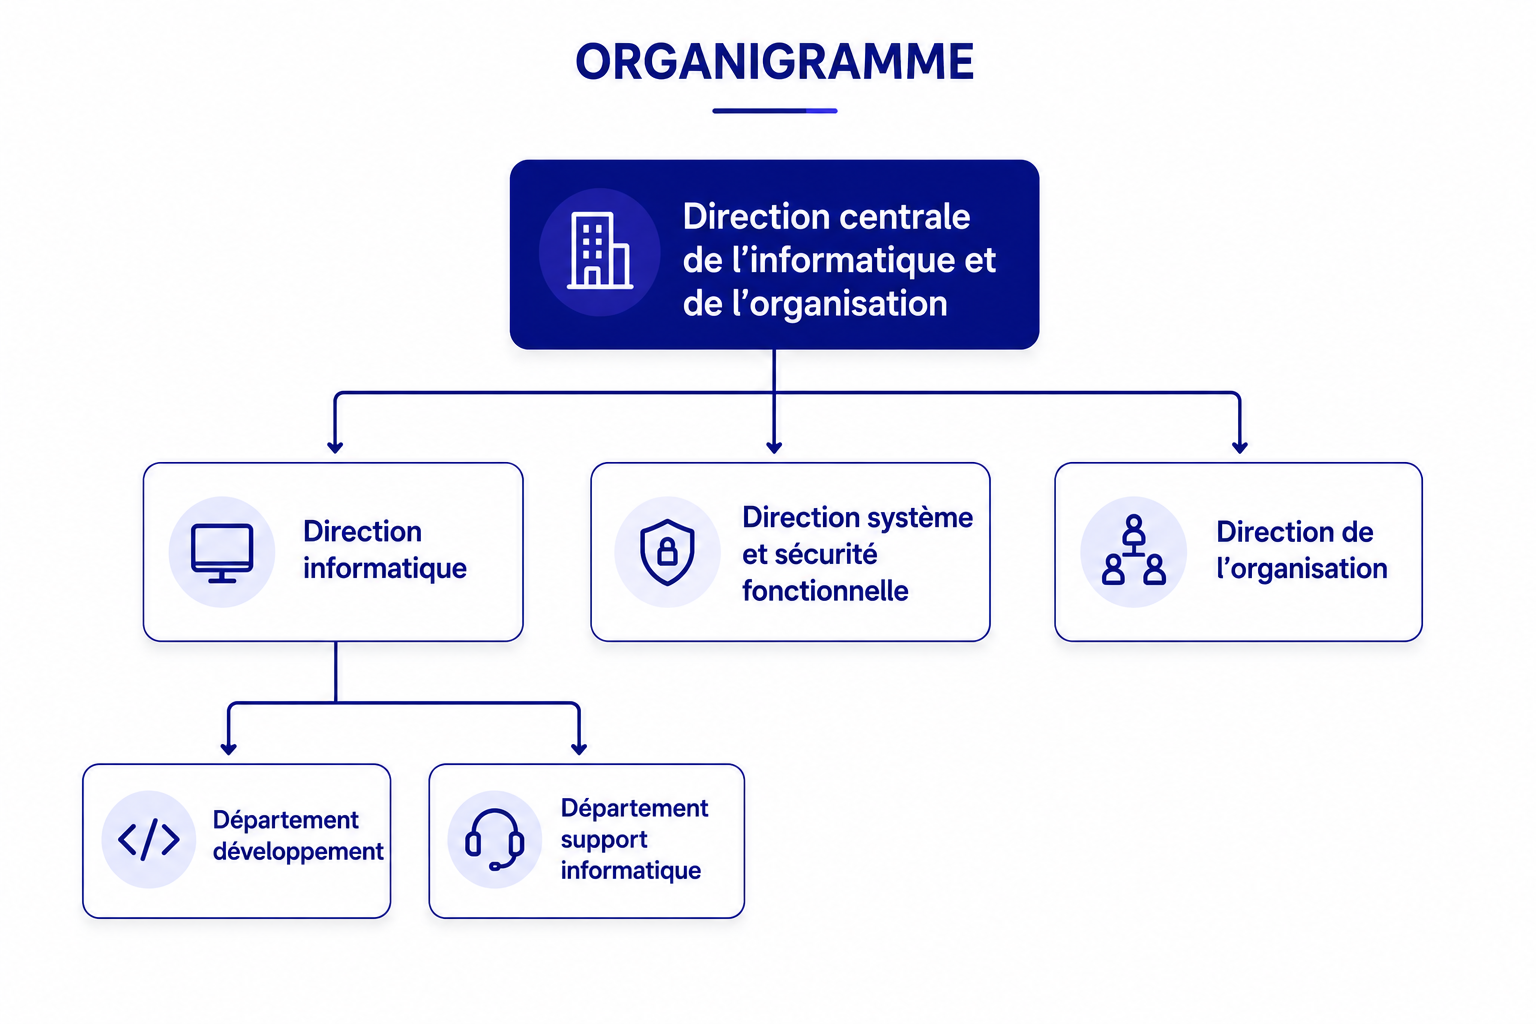
\includegraphics[width=0.75\textwidth]{images copy/image_ch1/organigramme.png}
  \caption{\textit{Organigramme de la Banque de Tunisie et des Émirats}}
  \label{fig:ch1-organigramme}
\end{figure}

Ancrée dans cette dynamique de digitalisation, la BTE fait face à un enjeu réglementaire et opérationnel central : la modernisation de son processus de vérification d'identité client, communément désigné sous le terme KYC.


%=============================================================
\section{Compréhension du métier KYC}
\label{sec:comprehension-kyc}
%=============================================================

Dans un secteur bancaire soumis à des exigences réglementaires croissantes, la maîtrise de l'identité client est devenue un impératif non négociable. Le KYC (\textit{Know Your Customer}), ou \og Connaissance du Client \fg{}, désigne l'ensemble des procédures permettant à un établissement financier d'authentifier ses clients et de se conformer aux normes de lutte contre le blanchiment d'argent et le financement du terrorisme (LCB-FT). Cette section examine d'abord les deux formes que prend ce processus --- traditionnel et automatisé --- avant de présenter le cadre réglementaire qui l'encadre.

\subsection{KYC traditionnel vs KYC automatisé}
\label{subsec:kyc-traditionnel-vs-automatise}

Cette sous-section confronte le modèle KYC traditionnel, entièrement manuel, à son évolution automatisée, afin de mettre en lumière les apports du e-KYC et de justifier l'orientation technologique du présent projet.

\subsubsection{Le KYC traditionnel}

Historiquement, le processus KYC repose sur des interactions physiques ou semi-numériques. Le client soumet des documents d'identité (Carte Nationale d'Identité, Passeport) qui sont ensuite contrôlés par des agents humains, selon deux modalités distinctes.

\paragraph{Processus hors ligne}
Dans ce mode, le client se déplace en agence pour remettre ses documents en main propre. L'agent de back-office procède à une vérification manuelle, saisit les données dans le système d'information et notifie le client de l'issue du contrôle. Ce processus séquentiel est visualisé à travers la Figure~\ref{fig:ch1-kyc-hors-ligne}.

\begin{figure}[H]
  \centering
  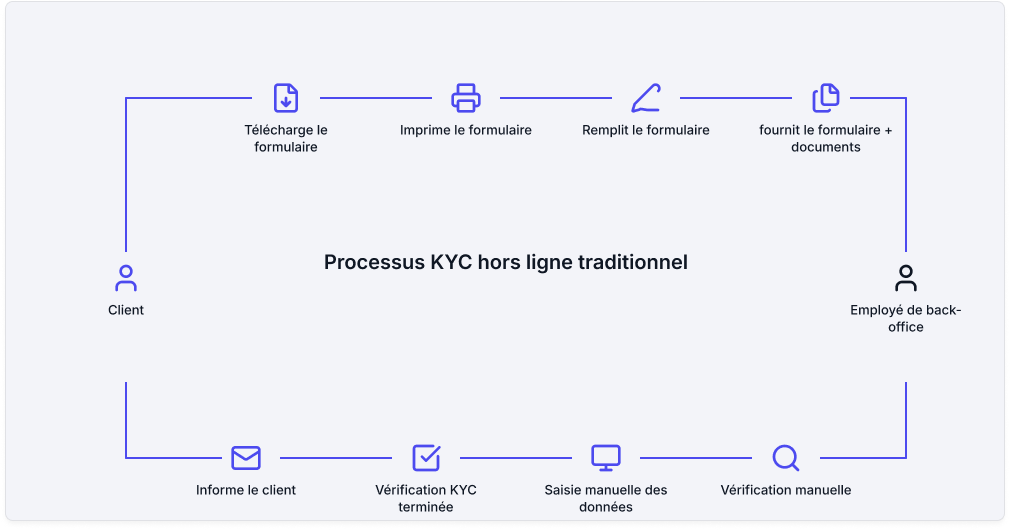
\includegraphics[width=0.75\textwidth]{images/image_ch1/SLIDE 1_ Hors ligne3.png}
  \caption{\textit{Processus KYC traditionnel hors ligne}}
  \label{fig:ch1-kyc-hors-ligne}
\end{figure}

\paragraph{Processus en ligne}
La variante en ligne, illustrée par la Figure~\ref{fig:ch1-kyc-en-ligne}, permet au client de soumettre ses documents via le portail numérique de l'établissement. Malgré la dématérialisation du canal, la vérification reste entièrement manuelle : un opérateur examine chaque pièce transmise avant de valider ou de rejeter le dossier.

\begin{figure}[H]
  \centering
  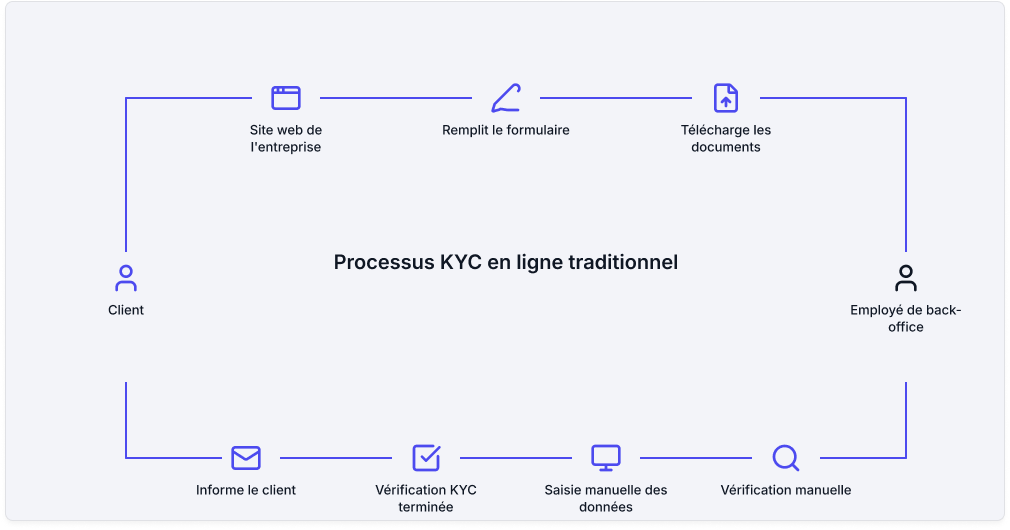
\includegraphics[width=0.75\textwidth]{images/image_ch1/SLIDE 2_ En ligne.png}
  \caption{\textit{Processus KYC traditionnel en ligne}}
  \label{fig:ch1-kyc-en-ligne}
\end{figure}

\paragraph{Limites structurelles du KYC traditionnel}
Qu'il soit réalisé en agence ou via un portail numérique, le KYC traditionnel présente des failles communes qui fragilisent son aptitude à répondre aux exigences croissantes des institutions financières modernes : des délais de traitement significatifs qui dégradent l'expérience client, un risque d'erreurs humaines lors de la saisie ou de la vérification manuelle pouvant induire des faux positifs ou des failles de conformité, et une mobilisation importante de ressources humaines difficiles à faire évoluer face à la croissance du portefeuille clients.

\subsubsection{Le KYC automatisé (e-KYC)}

Sous l'impulsion de la transformation digitale, les institutions financières migrent progressivement vers des solutions de e-KYC (\textit{Electronic KYC}). Cette approche substitue l'intervention humaine par des traitements algorithmiques intelligents, capables d'analyser, d'extraire et de valider les informations d'identité en temps réel. Ce nouveau paradigme repose sur un enchaînement fluide d'étapes entièrement automatisées, comme le montre la Figure~\ref{fig:ch1-kyc-automatise}.

\begin{figure}[H]
  \centering
  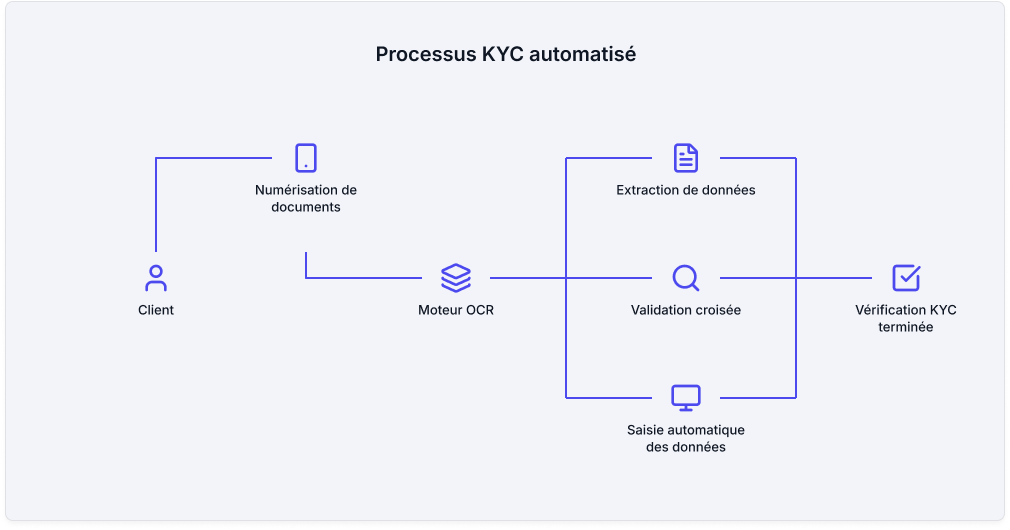
\includegraphics[width=0.75\textwidth]{images/image_ch1/SLIDE 3_ Automatis.png}
  \caption{\textit{Processus KYC automatisé}}
  \label{fig:ch1-kyc-automatise}
\end{figure}

Le workflow du e-KYC, tel qu'illustré par la figure ci-dessus, se déroule en quatre étapes enchaînées automatiquement :

\begin{enumerate}
  \item Numérisation des documents d'identité via smartphone ou scanner.
  \item Traitement par un moteur OCR pour l'extraction des données textuelles.
  \item Validation croisée et saisie automatique des données extraites dans le système.
  \item Vérification KYC complète, sans intervention humaine.
\end{enumerate}

Cette automatisation offre des avantages stratégiques concrets : un traitement quasi instantané contre plusieurs heures en mode manuel, une réduction des coûts back-office, une détection algorithmique et reproductible des fraudes documentaires, et un parcours 100\,\% digital disponible 24h/24 depuis n'importe quel appareil.

\subsection{Cadre réglementaire et normatif}
\label{subsec:cadre-reglementaire}

Toute solution de KYC automatisé doit s'inscrire dans un cadre légal rigoureux. Cette sous-section présente les normes internationales et les réglementations nationales tunisiennes qui encadrent le déploiement de la solution eKYC de la BTE.

\subsubsection{Normes internationales}

Déployer un système eKYC dans un environnement bancaire réglementé implique de respecter des standards internationaux qui définissent les obligations minimales en matière de vigilance client. Le Tableau~\ref{tab:normes-intl} présente les deux références les plus déterminantes pour le périmètre de ce projet.

\begin{longtable}{|p{3.8cm}|p{6cm}|p{4cm}|}
  \toprule
  \rowcolor{bleu_principal}
  \textcolor{white}{\textbf{Référence}} & \textcolor{white}{\textbf{Description}} & \textcolor{white}{\textbf{Source}} \\
  \midrule
  \endfirsthead
  \toprule
  \rowcolor{bleu_principal}
  \textcolor{white}{\textbf{Référence}} & \textcolor{white}{\textbf{Description}} & \textcolor{white}{\textbf{Source}} \\
  \midrule
  \endhead
  Groupe d'Action Financière (GAFI) --- Recommandation 10 &
  Organisme international fixant les standards mondiaux LCB-FT, notamment la vigilance client (\textit{Customer Due Diligence}). &
  {\scriptsize\textcolor{bleu_clair}{\url{https://www.fatf-gafi.org}}} \newline {\scriptsize\textit{Consulté le 18/03/2026}} \\
  \midrule
  Règlement Général sur la Protection des Données (RGPD) &
  Applicable aux solutions traitant des données de ressortissants ou de filiales de banques européennes. Exige la sécurisation des données biométriques et personnelles. &
  \begin{minipage}[t]{4cm}{\scriptsize\textit{Règlement (UE) 2016/679 du Parlement européen}}\newline{\scriptsize\textit{Consulté le 18/03/2026}}\end{minipage} \\
  \bottomrule
  \caption{Normes réglementaires internationales}
  \label{tab:normes-intl}
\end{longtable}

\subsubsection{Réglementations nationales (Tunisie)}

Au plan national, la solution eKYC de la BTE doit se conformer à un corpus législatif tunisien qui encadre à la fois l'identification des clients, le contrôle interne et la protection des données personnelles. Le Tableau~\ref{tab:normes-natl} en synthétise les textes fondateurs.

\begin{longtable}{|p{4cm}|p{5.5cm}|p{4cm}|}
  \toprule
  \rowcolor{bleu_principal}
  \textcolor{white}{\textbf{Référence}} & \textcolor{white}{\textbf{Description}} & \textcolor{white}{\textbf{Source}} \\
  \midrule
  \endfirsthead
  \toprule
  \rowcolor{bleu_principal}
  \textcolor{white}{\textbf{Référence}} & \textcolor{white}{\textbf{Description}} & \textcolor{white}{\textbf{Source}} \\
  \midrule
  \endhead
  Loi organique n°~2015-26 (modifiée par la loi n°~2019-9) &
  Texte fondateur imposant aux banques tunisiennes l'identification rigoureuse de leurs clients, en conformité avec les recommandations du GAFI. &
  {\scriptsize\textcolor{bleu_clair}{\href{https://www.ohchr.org/sites/default/files/lib-docs/HRBodies/UPR/Documents/Session27/TN/26Annexe16Loi2015_26fr.pdf}{ohchr.org --- Loi 2015-26}}}\newline{\scriptsize\textit{Consulté le 18/03/2026}} \\
  \midrule
  Circulaire de la Banque Centrale de Tunisie (BCT) n°~2018-09~\cite{bct2018circulaire} &
  Fixe les règles de contrôle interne et de conformité, obligeant les établissements à déployer des procédures de vigilance \textit{Know Your Customer}. &
  {\scriptsize\textcolor{bleu_clair}{\url{https://www.bct.gov.tn/bct/siteprod/documents/Cir_2025_06_fr.pdf}}} \newline {\scriptsize\textit{Consulté le 18/03/2026}} \\
  \midrule
  Loi organique n°~2004-63 --- Instance Nationale de Protection des Données Personnelles (INPDP) &
  Toute solution KYC collectant des images de CIN en Tunisie doit être déclarée à l'INPDP. Notre solution y répond via un traitement local, selon les principes de \textit{Privacy by Design}. &
  {\scriptsize\textcolor{bleu_clair}{\url{https://www.inpdp.tn/ressources/loi_2004.pdf}}} \newline {\scriptsize\textit{Consulté le 18/03/2026}} \\
  \midrule
  Commission Tunisienne des Analyses Financières (CTAF) / Banque Centrale de Tunisie (BCT) / Conseil du Marché Financier (CMF) &
  Principaux régulateurs supervisant respectivement la conformité LCB-FT et les rapports de transactions suspectes, les institutions financières, et les marchés de capitaux. &
  \begin{minipage}[t]{3.8cm}
    {\scriptsize\textcolor{bleu_clair}{\url{https://www.ctaf.gov.tn}}}\newline
    {\scriptsize\textcolor{bleu_clair}{\url{https://www.bct.gov.tn}}}\newline
    {\scriptsize\textcolor{bleu_clair}{\url{https://www.cmf.tn}}}\newline
    {\scriptsize\textit{Consultés le 18/03/2026}}
  \end{minipage} \\
  \bottomrule
  \caption{Réglementations nationales tunisiennes}
  \label{tab:normes-natl}
\end{longtable}

Le passage du KYC traditionnel vers le e-KYC représente une rupture profonde dans la gestion de l'identité client : en substituant les traitements manuels par des pipelines intelligents (OCR, vision par ordinateur, intelligence artificielle) les établissements financiers gagnent en rapidité, en précision et en conformité. Encadrée par un corpus réglementaire solide, cette évolution s'impose désormais comme un levier stratégique incontournable pour toute institution souhaitant conjuguer efficacité opérationnelle et robustesse réglementaire.


%=============================================================
\section{Position du problème}
\label{sec:position-probleme}
%=============================================================

Cette section analyse l'existant à deux niveaux : d'abord le processus KYC interne de la BTE et ses faiblesses, puis les solutions commerciales disponibles sur le marché et leurs limites dans le contexte spécifique de la banque. Cette double analyse conduit à formuler la problématique centrale du projet.

\subsection{KYC interne de la BTE et analyse critique}
\label{subsec:etude-existant}

Cette sous-section examine le fonctionnement actuel du processus KYC au sein de la BTE, puis en dresse un bilan critique pour identifier les failles structurelles qui justifient l'automatisation.

\subsubsection{KYC au sein de la BTE}

Au sein de la BTE, le processus KYC s'articule autour de deux modes complémentaires : un traitement réalisé en agence et un parcours digital accessible via l'application mobile NEO BTE. Ces deux modes, dont le fonctionnement détaillé a été présenté en section~\ref{subsec:kyc-traditionnel-vs-automatise}, sont ici examinés sous l'angle de leur mise en œuvre concrète au sein de l'établissement. Si ces deux canaux couvrent des usages distincts, ils partagent une caractéristique fondamentale : tous deux reposent entièrement sur une vérification manuelle par des agents humains, sans aucune automatisation du traitement documentaire. La Figure~\ref{fig:ch1-kyc-modes} met en regard ces deux modalités et souligne leur dénominateur commun : la dépendance à l'intervention humaine.

\begin{figure}[H]
  \centering
  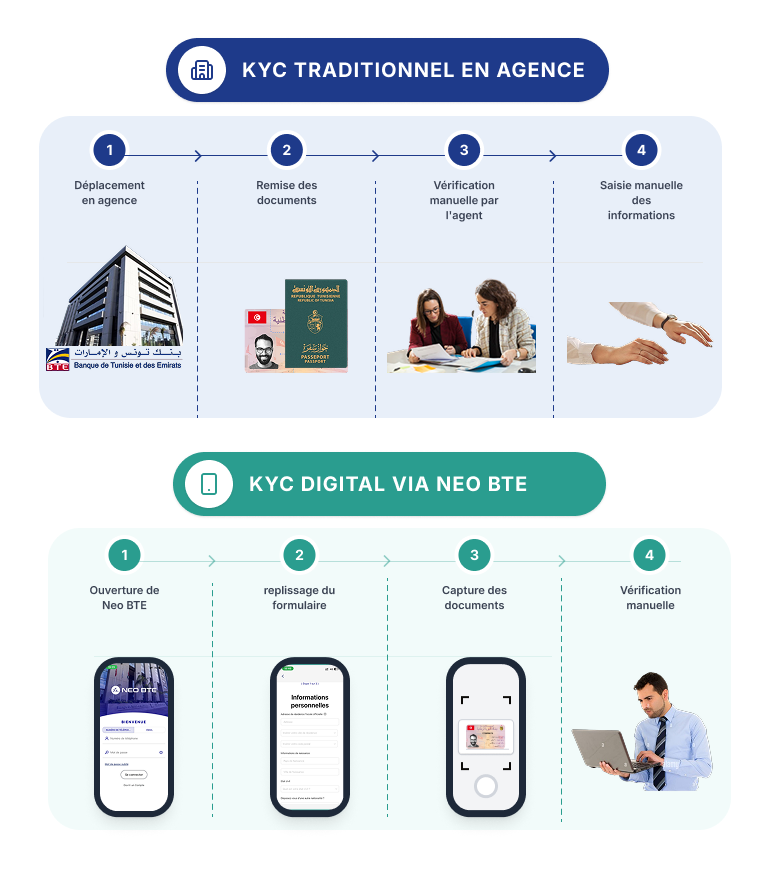
\includegraphics[width=0.75\textwidth]{images/image_ch1/KYC_Agence_Vs_NeoBte.png}
  \caption{\textit{KYC Traditionnel en agence vs Digital via NEO BTE}}
  \label{fig:ch1-kyc-modes}
\end{figure}

\subsubsection{Analyse critique du processus interne}

L'examen du processus KYC interne met en évidence quatre failles structurelles majeures.

\begin{itemize}
  \item \textbf{Délais incompatibles avec le digital :} la vérification manuelle impose des temps de traitement qui dégradent l'expérience d'onboarding et contrastent avec les attentes d'un client NEO BTE habitué à l'instantané.
  \item \textbf{Faillibilité humaine :} les erreurs de saisie et d'appréciation visuelle sont inévitables à grande échelle, pouvant générer des faux positifs ou des omissions de conformité engageant la responsabilité de la banque vis-à-vis de la BCT.
  \item \textbf{Vulnérabilité à la fraude documentaire :} face à des documents retouchés ou des identités usurpées, l'œil humain ne peut garantir une détection systématique et reproductible.
  \item \textbf{Difficulté de passage à l'échelle :} le modèle manuel ne peut absorber la croissance du portefeuille clients NEO BTE sans une augmentation proportionnelle des effectifs, rendant le système structurellement non scalable.
\end{itemize}

\subsection{Solutions KYC commerciales et leurs limites}
\label{subsec:solutions-commerciales}

Face aux faiblesses du processus interne, trois plateformes représentatives du marché ont été étudiées pour évaluer leur pertinence dans le contexte spécifique de la BTE. Chacune a été analysée selon des critères déterminants (couverture fonctionnelle, support du contexte tunisien, dépendance cloud et personnalisabilité ).

\subsubsection{Présentation des solutions étudiées}

Trois plateformes ont été analysées selon des critères déterminants pour le contexte de la BTE.

\paragraph{uqudo~\cite{uqudo2026}}
Plateforme complète intégrant OCR, biométrie et détection de fraude, accessible via une API cloud avec support multilingue. Elle couvre un périmètre fonctionnel large mais repose entièrement sur une infrastructure externe.

\paragraph{NEUROPARSER~\cite{neuroparser2026}}
Solution spécialisée dans l'OCR de la carte d'identité nationale tunisienne. Bien qu'elle offre un support natif de la CIN, son périmètre se limite à l'extraction de données textuelles, sans capacités biométriques ni détection d'anomalies.

\paragraph{FACEKI~\cite{faceki2026}}
Solution orientée vers la vérification biométrique et l'analyse documentaire, offrant des garanties de sécurité avancées, mais dépendant entièrement d'une infrastructure cloud externe.

Le Tableau~\ref{tab:solutions-kyc} synthétise cette analyse comparative selon les critères les plus déterminants pour le contexte de la BTE.

\begin{table}[H]
  \centering
  \small
  \begin{tabular}{|l|c|c|c|}
    \toprule
    \rowcolor{bleu_principal}
    \textcolor{white}{\textbf{Critère}} & \textcolor{white}{\textbf{uqudo}} & \textcolor{white}{\textbf{NEUROPARSER}} & \textcolor{white}{\textbf{FACEKI}} \\
    \midrule
    Périmètre fonctionnel & AML + Biométrie & OCR uniquement & Biométrie + Docs \\
    \midrule
    \rowcolor{gris_leger}
    Support CIN tunisienne & Partiel & \textbf{OUI} & Partiel \\
    \midrule
    Détection de fraude & \textbf{OUI} & NON & \textbf{OUI} \\
    \midrule
    \rowcolor{gris_leger}
    Intégration API & \textbf{OUI} & \textbf{OUI} & \textbf{OUI} \\
    \midrule
    Sensibilité qualité image & Modérée & Élevée & Modérée \\
    \midrule
    \rowcolor{gris_leger}
    Dépendance cloud & Forte & Forte & Forte \\
    \midrule
    Coût & Élevé & Modéré & Élevé \\
    \midrule
    \rowcolor{gris_leger}
    Personnalisation & Limitée & Limitée & Limitée \\
    \bottomrule
  \end{tabular}
  \caption{Comparaison des solutions KYC commerciales : uqudo, NEUROPARSER et FACEKI}
  \label{tab:solutions-kyc}
\end{table}

\subsubsection{Limites par rapport au contexte de la BTE}

L'analyse comparative révèle que les trois solutions partagent des limites rédhibitoires pour la BTE.

\begin{itemize}
  \item \textbf{Dépendance cloud systématique :} les trois plateformes analysées transmettent les données documentaires vers des serveurs externes, soulevant des enjeux de souveraineté des données incompatibles avec les exigences d'un établissement bancaire réglementé.
  \item \textbf{Inadaptation au contexte tunisien :} le traitement bilingue arabe/latin, propre à la CIN et au passeport tunisiens, n'est que partiellement ou non pris en charge, dégradant la fiabilité de l'extraction.
  \item \textbf{Coûts, rigidité et dépendance stratégique :} les licences propriétaires sont élevées, les modèles ne sont pas personnalisables et aucune adaptation aux évolutions des documents nationaux ou aux exigences de la BCT n'est possible, privant la BTE de toute autonomie sur l'évolution de son système.
  \item \textbf{Sensibilité aux conditions de capture mobile :} la qualité variable des images prises en situation réelle entraîne des taux d'échec significatifs, non compensés par des mécanismes de robustesse intégrés.
\end{itemize}

Ces constats convergent vers une conclusion sans appel : ni le processus interne actuel, ni les solutions propriétaires disponibles ne sont en mesure de répondre aux ambitions portées par la stratégie NEO BTE.

\subsection{Problématique }
\label{subsec:problematique}

L'ensemble des faiblesses identifiées converge vers une problématique unique, à la fois opérationnelle et stratégique. Le KYC manuel constitue aujourd'hui un frein structurel à la stratégie digitale de la BTE : il est incapable de répondre à la montée en charge qu'exige la croissance rapide du portefeuille clients NEO BTE, il compromet la fluidité du parcours d'onboarding et alourdit les coûts de traitement, et il fragilise la posture de conformité de l'établissement face aux exigences de la BCT. Parallèlement, les solutions commerciales analysées s'avèrent inadaptées aux contraintes réglementaires, documentaires et de souveraineté des données propres au contexte tunisien. Ce double constat impose de formuler la question centrale suivante :

\begin{quote}
\textit{\textbf{Comment concevoir une solution KYC automatisée, internalisée et adaptée au contexte tunisien, capable d'extraire, de classifier et de valider des documents d'identité avec fiabilité, tout en garantissant la conformité aux directives de la BCT et la souveraineté des données de la BTE ?}}
\end{quote}

Cette problématique engage trois défis techniques majeurs : l'extraction précise de données textuelles sur des documents multilingues et de qualité variable, la robustesse du système face aux conditions réelles de capture mobile, et l'intégration du module IA dans un \textit{workflow} bancaire structuré, modulaire et auditable.

\subsection{Solution proposée}
\label{subsec:solution-proposee}

Le présent projet propose de concevoir un système eKYC développé sur mesure pour la BTE, dont le c\oe{}ur est un pipeline d'intelligence artificielle automatisé. Avant même la soumission du dossier, le système détecte automatiquement le type de document présenté (CIN, passeport). Dès la soumission, il prend en charge sans action manuelle l'extraction des données par reconnaissance optique de caractères (OCR), la vérification de cohérence des informations extraites, et la détection d'anomalies et de tentatives de fraude documentaire. Ce traitement bout-en-bout garantit une réponse quasi instantanée et reproductible, là où l'opérateur humain introduisait latence et variabilité.

Toutefois, tout système d'IA présente des marges d'erreur résiduelles. C'est pourquoi l'intervention humaine est maintenue comme verrou de décision finale : un agent bancaire conserve la validation ultime sur les dossiers signalés ou ambigus. Le rôle de l'IA est d'assister et d'accélérer l'agent, non de le remplacer intégralement. La solution repose sur trois piliers : une architecture \textit{on-premise} garantissant qu'aucune donnée documentaire ne quitte l'infrastructure bancaire, une adaptation native au contexte tunisien avec des modèles entraînés sur des documents bilingues arabe/latin (CIN, passeport), et une stack entièrement open-source assurant une autonomie totale sur l'évolution du système.


%=============================================================
\section{Méthodologie adoptée }
\label{sec:methodologie}
%=============================================================

Ce projet présente une double nature : d'un côté, un travail de recherche appliquée en intelligence artificielle, soumis à l'incertitude expérimentale ; de l'autre, le développement d'une plateforme bancaire fonctionnelle, aux exigences stables et formalisables. Ni les frameworks purement scientifiques, ni les méthodologies classiques de génie logiciel ne permettent, pris isolément, de répondre efficacement à ces deux dimensions. Une approche hybride a donc été retenue, structurée en deux incréments distincts, chacun piloté par le modèle le plus adapté à sa nature propre.

\subsection{Modèle incrémental}
\label{subsec:modele-incremental}

Le modèle incrémental consiste à construire un système par ajouts successifs et fonctionnels, appelés incréments. Cette approche permet de prioriser les composantes les plus critiques dès le départ, de valider indépendamment chaque bloc avant d'aborder le suivant, et de réduire les risques d'intégration en fin de projet. Ce choix est naturellement justifié par la double complexité du projet, qui se décline selon deux composantes de natures fondamentalement différentes : une composante Intelligence Artificielle (vision par ordinateur, OCR, scoring de documents), caractérisée par une forte incertitude expérimentale et une dépendance importante à la qualité des données d'entraînement, et une composante développement logiciel (backend, frontend, workflow bancaire), nécessitant une architecture claire et une intégration progressive des fonctionnalités. Ces deux composantes présentant une faible interdépendance technique, leur structuration en deux incréments distincts s'impose, tout en préservant la cohérence globale du système livré.

\subsection{CRISP-ML(Q)}
\label{subsec:crisp-mlq}

CRISP-ML(Q) est le modèle retenue pour piloter le premier incrément, consacré au développement du pipeline IA. Cette sous-section en présente les fondements et les six phases structurantes.

\subsubsection{CRISP-ML(Q) vs CRISP-DM}

Avant d'aller plus loin, il convient de situer CRISP-ML(Q) par rapport à son prédécesseur. CRISP-DM (\textit{Cross-Industry Standard Process for Data Mining}), publié en 1999, a longtemps constitué la référence méthodologique pour les projets de fouille de données. Cependant, son adoption aux projets de Machine Learning en production révèle plusieurs lacunes : l'absence de phases dédiées au déploiement continu, à la surveillance en production et, surtout, à l'assurance qualité systématique tout au long du cycle de vie du modèle. CRISP-ML(Q) (\textit{Cross-Industry Standard Process for Machine Learning with Quality Assurance}) comble précisément ces lacunes. Proposé en 2020 par Studer \textit{et al.}~\cite{studer2021crispmlq} , le modèle introduit le \og Q \fg{} pour \textit{Quality} comme philosophie transversale : des contrôles qualité formels sont intégrés à chaque phase du processus, et non uniquement lors de l'évaluation finale. Cette dimension qualité renforcée est particulièrement précieuse dans un contexte bancaire où la fiabilité et l'auditabilité des systèmes IA sont des exigences non négociables.

\subsubsection{Les six phases de CRISP-ML(Q)}

Le 1\textsuperscript{er} incrément du projet est entièrement dédié à la conception, à l'entraînement et à la validation du pipeline d'intelligence artificielle, selon le cadre CRISP-ML(Q). La Figure~\ref{fig:ch1-6-phases-crisp-mlq} présente les six phases qui structurent ce cycle.

\begin{figure}[H]
  \centering
  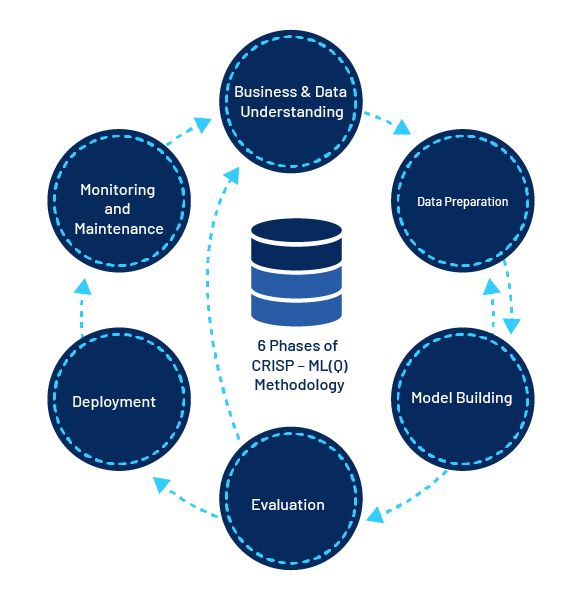
\includegraphics[width=0.75\textwidth]{images/image_ch1/crispMl_Q.png}
  \caption{\textit{Les six phases du modèle CRISP-ML(Q)}}
  \label{fig:ch1-6-phases-crisp-mlq}
\end{figure}

\begin{enumerate}
  \item \textbf{Business \& Data Understanding :} analyse des besoins métiers, identification des types de documents à traiter (CIN, passeport), ainsi que constitution et caractérisation du jeu de données. Un contrôle qualité initial vérifie la représentativité et la pertinence des données collectées.
  \item \textbf{Data Preparation :} nettoyage, transformation, organisation et préparation des données afin de les rendre exploitables pour l'apprentissage. Des métriques qualité sont appliquées pour valider chaque transformation opérée sur le corpus documentaire.
  \item \textbf{Modeling :} entraînement et optimisation des modèles de Deep Learning répondant au problème identifié. Les expériences sont tracées et comparées selon des critères de qualité prédéfinis, garantissant la reproductibilité des résultats.
  \item \textbf{Evaluation \& Quality Assurance :} mesure des performances du modèle et vérification de son adéquation avec les objectifs métier fixés. Cette phase constitue le verrou qualité central avant tout passage en production.
  \item \textbf{Deployment \& Integration :} intégration du modèle validé dans l'architecture applicative. Des tests de non-régression et des vérifications de conformité réglementaire accompagnent cette mise en production.
  \item \textbf{Monitoring \& Maintenance :} suivi continu du modèle déployé, détection des dérives de performance (\textit{data drift}) et maintenance évolutive face aux évolutions des documents et des conditions de capture.
\end{enumerate}

À l'issue de cet incrément, le résultat attendu est un moteur IA opérationnel, capable de détecter les documents soumis, d'en extraire les informations structurées et de fonctionner de manière fiable en conditions réelles, avec des garanties qualité documentées à chaque étape.

\subsection{Modèle en cascade}
\label{subsec:modele-cascade}

Une fois le c{\oe}ur IA validé, le second incrément se consacre au développement de la plateforme applicative dans son intégralité. Pour cette composante logicielle, dont les exigences fonctionnelles sont clairement définies et stables dès le départ, le modèle en cascade s'impose comme le cadre le plus adapté. Il s'agit d'une approche séquentielle et structurée dans laquelle chaque phase doit être achevée et validée avant que la suivante ne commence, garantissant une traçabilité complète des décisions de conception. Appliqué à l'incrément applicatif, il se décline selon les phases suivantes :

\begin{enumerate}
  \item \textbf{Analyse des besoins :} recueil et formalisation des exigences fonctionnelles et non fonctionnelles du système (interfaces agent et client, workflow KYC, intégration du module IA).
  \item \textbf{Conception :} définition de l'architecture logicielle, des modèles de données et des interfaces utilisateur.
  \item \textbf{Implémentation :} développement du back-office destiné aux agents bancaires (gestion des dossiers, supervision des validations, tableau de bord KYC) et du front-office permettant aux clients de soumettre leurs documents et de suivre l'état de leur dossier en temps réel.
  \item \textbf{Intégration \& Tests :} connexion de la plateforme applicative au pipeline intelligent développé lors de l'incrément 1, tests \textit{end-to-end} et validation du système complet.
  \item \textbf{Déploiement :} livraison du système intégré dans l'environnement bancaire cible.
\end{enumerate}

Ce modèle est particulièrement approprié ici car les spécifications du module applicatif sont suffisamment précises et stables pour éviter les allers-retours coûteux que justifieraient des méthodes itératives. Il offre par ailleurs une visibilité claire sur l'avancement du projet et facilite la communication avec les parties prenantes de la BTE.

\subsection{Planification globale du projet}
\label{subsec:planification}

L'approche incrémentale hybride retenue se traduit concrètement par une planification en deux phases successives et cohérentes. La Figure~\ref{fig:ch1-planning} illustre la répartition temporelle des grandes activités du projet selon les deux incréments et leurs jalons principaux.

\begin{figure}[H]
  \centering
  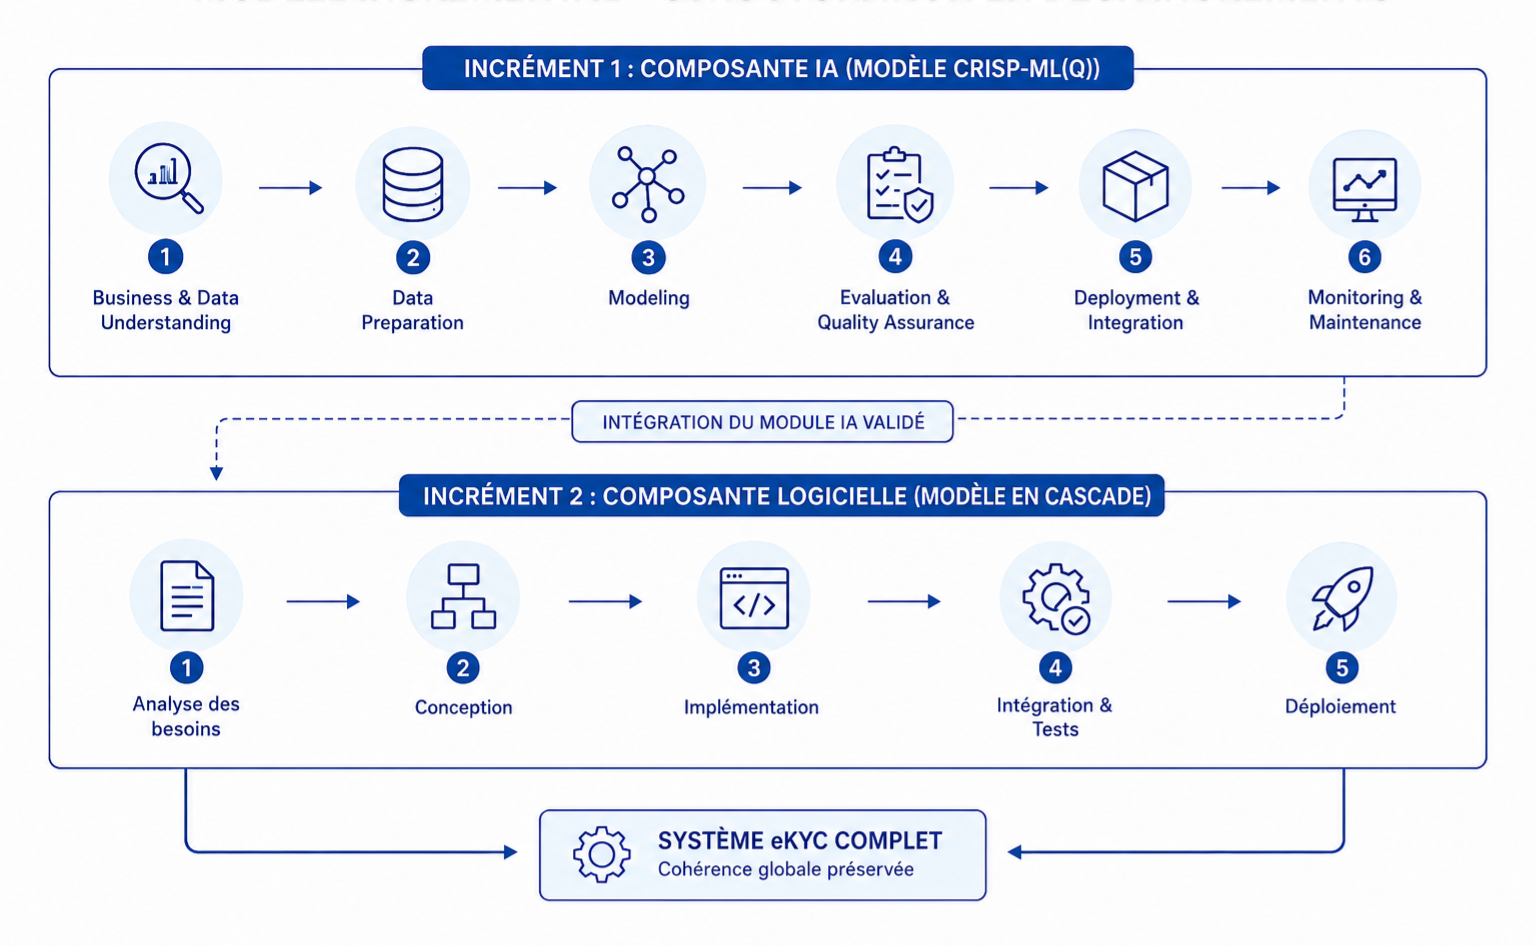
\includegraphics[width=\textwidth]{images/image_ch1/plannification du travail.PNG}
  \caption{\textit{Planification globale du projet selon l'approche incrémentale hybride}}
  \label{fig:ch1-planning}
\end{figure}

Cette structuration garantit que le module IA (composante la plus critique et la plus incertaine du projet) est pleinement validé avant d'être intégré à la plateforme applicative, réduisant ainsi les risques d'échec en phase d'intégration et assurant une livraison finale maîtrisée.


\section*{Conclusion du chapitre}

Ce chapitre a posé l'ensemble du cadre général du projet : présentation de la BTE et de sa plateforme NEO BTE, compréhension du métier KYC et de son cadre réglementaire, puis analyse critique des pratiques internes et des solutions commerciales disponibles. De ces analyses découle une problématique claire : l'incapacité du dispositif KYC actuel à assurer le passage à l'échelle qu'exige la stratégie digitale de la BTE, à laquelle répond une solution interne \textit{on-premise}, open-source et adaptée au contexte tunisien. La méthodologie hybride retenue garantit une structuration rigoureuse du développement en deux incréments complémentaires, dont les chapitres suivants détailleront les réalisations.


% ============================================================
% CHAPITRE 2  (Spécification — hors partie)
% ============================================================

% =============================================
% CHAPITRE 4 — INCRÉMENT 2
% =============================================

\chapter{Spécification des Besoins et Architecture}
\label{chap:specification-architecture}
\vspace{1em}
\noindent\textbf{\large Sommaire}
\vspace{0.5em}
\localtableofcontents
\clearpage

Ce chapitre pose les fondements de la phase de réalisation du système eKYC. Il commence par identifier les acteurs impliqués et formaliser l'ensemble des besoins fonctionnels et non fonctionnels de la plateforme, puis décrit l'architecture logique et physique retenue pour y répondre. L'ensemble est consolidé par un diagramme de cas d'utilisation global et la description détaillée de chaque interaction, constituant ainsi le référentiel de conception sur lequel s'appuient les chapitres de réalisation suivants.

%=============================================================
\section{Spécification des besoins}
\label{sec:specification-besoins}
%=============================================================

\subsection{Identification des acteurs}
\label{subsec:identification-acteurs}

Le système eKYC développé dans ce projet met en interaction plusieurs acteurs aux responsabilités bien distinctes. Le Tableau~\ref{tab:acteurs_pfe} présente chaque acteur, sa nature et son rôle au sein de la plateforme.

\renewcommand{\arraystretch}{1.5}
\begin{longtable}{|>{\bfseries}p{3.8cm}|p{10.2cm}|}
  \hline
  \rowcolor{bleu_clair!20}
  \textbf{Acteur} & \textbf{Rôle et responsabilités} \\
  \hline
  \endfirsthead
  \hline
  \rowcolor{bleu_clair!20}
  \textbf{Acteur} & \textbf{Rôle et responsabilités} \\
  \hline
  \endhead
    Client & 
      Particulier souhaitant ouvrir un compte bancaire. Interagit exclusivement avec l'interface client, accessible sur mobile et navigateur web. Soumet ses documents d'identité, peut corriger les données extraites et réalise la capture biométrique. \\
    \hline
    Analyste KYC & 
      Agent opérationnel de la BTE chargé d'examiner les dossiers traités par le système IA. Consulte les données extraites, les résultats du filtrage AML (\textit{Anti-Money Laundering} / Lutte contre le blanchiment d'argent) et le score de risque, puis prend la décision finale de validation, de rejet ou de demande de complément. \\
    \hline
    Administrateur & 
      Profil à droits étendus qui possède les mêmes fonctionnalités que l'analyste KYC et le responsable qualité du système IA. Consulte le journal d'audit dans son intégralité. \\
    \hline
    Responsable qualité IA & 
      Profil technique chargé de surveiller en continu les performances des modèles d'intelligence artificielle. Consulte les indicateurs de qualité par type de document et par modèle. N'accède à aucune donnée personnelle du client. \\
    \hline
  
  \caption{Acteurs et périmètres d'action du système eKYC}
  \label{tab:acteurs_pfe}
\end{longtable}

\subsection{Besoins fonctionnels}
\label{subsec:besoins-fonctionnels}

Les exigences fonctionnelles définissent les fonctionnalités clés que le système doit fournir pour satisfaire les besoins des utilisateurs.

\paragraph*{S'inscrire}
\begin{itemize}
  \item Créer un compte sur l'application (inscription classique).
\end{itemize}
\paragraph*{S'authentifier}
\begin{itemize} 
  \item Se connecter à la plateforme avec ses identifiants. 
\end{itemize}

\paragraph*{Soumettre et suivre un dossier KYC}
\begin{itemize}
  \item Initier un dossier KYC et choisir le type de document à soumettre (CIN ou passeport).
  \item Capturer son document guidé par un retour visuel en temps réel~; le système détecte automatiquement la présence, le type et la qualité du document via YOLOv8n avant de déclencher la capture.
  \item Consulter et peut corriger les informations extraites automatiquement par le pipeline OCR (YOLOv11m + PaddleOCR) avant soumission finale.
  \item Capturer un selfie biométrique avec un retour visuel en temps réel pour garantir un cadrage conforme au format requis.
  \item Suivre l'état de son dossier .
\end{itemize}

\paragraph*{Demander des services bancaires}

\noindent Une fois son dossier KYC approuvé et son compte bancaire courant ouvert, le client peut :

\begin{itemize}
  \item Soumettre une demande de carte bancaire.
  \item Soumettre une demande de chéquier.
  \item Soumettre une demande de crédit avec le document justificatif requis (attestation de salaire).
  \item Suivre l'état de ses demandes en cours.
\end{itemize}

\paragraph*{Traiter les dossiers KYC}
\begin{itemize}
  \item Consulter la file de traitement des dossiers en attente.
  \item Accéder au détail d'un dossier : données extraites, score de risque, résultat de la comparaison biométrique et alertes AML.
  \item Valider un dossier si les informations sont correctes et le score satisfaisant.
  \item Corriger manuellement un champ extrait erroné avant validation.
  \item Rejeter un dossier en documentant obligatoirement le motif de refus.
  \item demander des informations complémentaires au client en précisant les pièces manquantes ou les corrections à apporter.
\end{itemize}

\paragraph*{Administrer et surveiller la plateforme}
\begin{itemize}
  \item Consulter le registre global de tous les dossiers, tous statuts confondus.
  \item Consulter le journal d'audit immuable de toutes les actions effectuées.
  \item Consulter les indicateurs de performance des modèles IA .
 
\end{itemize}

\bigskip
\noindent L'analyse des besoins révèle que le système eKYC combine deux natures de travail complémentaires : un pipeline IA qui exige une phase de recherche, d'entraînement et de validation avant tout déploiement, et une plateforme applicative dont la réalisation dépend directement des résultats de ce pipeline. Cette interdépendance justifie l'adoption d'un \textbf{modèle de développement incrémental en deux incréments} : le premier consacré à la conception et à la validation du module IA, le second à la réalisation de la plateforme.

\subsection{Besoins non fonctionnels}
\label{subsec:besoins-non-fonctionnels}

Les besoins non fonctionnels définissent les caractéristiques essentielles que doit respecter le système, indépendamment des fonctionnalités métier.

\begin{description}[style=nextline, leftmargin=0pt, labelwidth=!, font=\bfseries\color{black}]

  \item[Sécurité]
  Bien que le cadre de ce projet académique n'impose pas de contraintes de sécurité formelles, nous avons fait le choix d'intégrer des mécanismes de sécurité qui se rapprochent au maximum des standards appliqués en environnement bancaire réel. La plateforme manipule des données d'identité sensibles comme les numéros de CIN, les photos de documents et les selfies, ce qui nous a guidés vers l'adoption de bonnes pratiques dès la conception. L'authentification repose sur des tokens JWT dont la durée de validité est limitée à 60 minutes, les mots de passe sont stockés sous forme hachée avec l'algorithme bcrypt, et les tokens sont révoqués immédiatement à la déconnexion. Les agents et administrateurs disposent d'un circuit d'authentification distinct des clients. Une double authentification est mise en place pour les actions critiques : toute décision sur un dossier nécessite une confirmation du mot de passe avant d'être enregistrée. Toutes les actions sensibles comme la connexion, la décision sur un dossier et la modification de paramètres sont tracées dans un journal d'audit horodaté et non modifiable.
  \item[Confidentialité des données]
  Dans le cadre de ce projet, l'ensemble de la plateforme est déployé en environnement local, simulant les conditions réelles d'un système bancaire où toutes les données restent confinées à l'infrastructure interne de la banque et ne transitent jamais vers l'extérieur. Cette approche reproduit le principe de souveraineté des données qu'une banque applique en production : les photos de documents, les selfies et les données d'identité des clients ne quittent jamais le périmètre du système. Les images sont stockées sur un serveur de fichiers local, et chaque composant y accède directement via une adresse interne sans exposition vers un réseau externe. Les résultats OCR contenant les données d'identité sont conservés temporairement côté client, puis transmis en une seule requête au backend lors de la soumission finale du dossier.
  \item[Conformité réglementaire]
  La plateforme eKYC a été conçue en conformité avec la \textbf{circulaire aux banques n°2025-06 du 28 février 2025} de la Banque Centrale de Tunisie, relative aux règles minimales régissant l'enrôlement électronique des clients~\cite{bct2025circ06}. Conformément aux exigences de cette circulaire, la plateforme met en oeuvre un processus d'identification électronique complet : collecte et vérification des documents d'identité du client, confirmation de la présence réelle du client par reconnaissance faciale (Article 6), filtrage et profilage du risque de chaque client (Article 7), et génération automatique d'une fiche d'identification KYC à l'issue du parcours (Article 8). La plateforme respecte également l'exigence de vigilance proportionnelle au profil de risque (Article 3) en attribuant à chaque dossier un niveau de risque (faible, moyen, élevé ou critique) qui détermine la décision de validation ou de revue manuelle par un agent.

  \item[Performance]
  Le système est conçu pour minimiser le temps de traitement perçu par le client à chaque étape du parcours KYC. Les modèles d'intelligence artificielle YOLO et PaddleOCR sont chargés en mémoire une seule fois au démarrage de chaque service et réutilisés pour toutes les requêtes suivantes, évitant ainsi tout rechargement coûteux. La détection en temps réel lors de la capture des documents s'exécute en moins de 20 ms par frame sur GPU, assurant une expérience fluide devant la caméra. Le pipeline OCR complet sur une CIN recto s'exécute en moyenne en [X] ms, en [X] ms pour le verso, et en [X] ms pour un passeport.


  \item[Maintenabilité]
  L'architecture modulaire permet de faire évoluer chaque composant indépendamment des autres. En particulier, le module IA peut être mis à jour ou remplacé sans impact sur la plateforme applicative, ce qui facilite les opérations de maintenance et les évolutions futures.
  \item[Extensibilité]
  La plateforme est conçue pour accueillir de nouveaux services bancaires sans restructuration de l'architecture existante. L'ajout d'un nouveau type de demande comme le crédit, la carte bancaire ou le chéquier suit le même schéma : un groupe de routes dédié dans le backend, un modèle de données indépendant et une interface client spécifique. Les services IA sont également extensibles : un nouveau type de document ou un nouveau modèle de détection peut être intégré comme un module supplémentaire sur un port dédié, sans modifier les services existants.

  \item[Accessibilité]
  Les interfaces sont conçues pour être intuitives et accessibles. L'interface client est disponible sur mobile et navigateur web sans installation. L'interface d'administration est ergonomique et structurée selon les rôles, permettant à chaque profil d'accéder rapidement aux fonctionnalités qui le concernent.

  \item[Auditabilité]
  Chaque action significative réalisée sur la plateforme est enregistrée dans un journal d'audit horodaté et non modifiable. Cela inclut les connexions et déconnexions des agents, les décisions prises sur les dossiers KYC (validation, rejet, demande de complément) De plus, toutes les corrections apportées aux données OCR, qu'elles proviennent du client ou d'un agent, sont conservées dans un historique dédié, permettant de retracer l'origine de chaque donnée utilisée dans la décision finale.

\end{description}


%=============================================================
\section{Architecture globale de la solution}
\label{sec:architecture-globale}
%=============================================================

L'architecture de la plateforme eKYC est conçue pour répondre simultanément aux contraintes de performance, de souveraineté des données et de modularité. Elle se décline en deux niveaux complémentaires : une vue logique qui organise les composants fonctionnels du système, et une vue physique qui décrit leur déploiement matériel concret.

\subsection{Architecture logique}
\label{subsec:architecture-logique}

 l'architecture logique de la plateforme eKYC, présentée dans la Figure~\ref{fig:ch4-archi-logique}, met en évidence en évidence les quatre couches fonctionnelles qui structurent le système ainsi que les flux de communication entre elles. On y distingue la couche présentation regroupant les interfaces utilisateur, la couche intelligence artificielle constituée des modules de capture et d'analyse, la couche backend centralisant la logique métier et l'authentification, et enfin la couche données assurant la persistance des informations.

\vspace{0.6em}
\begin{center}
  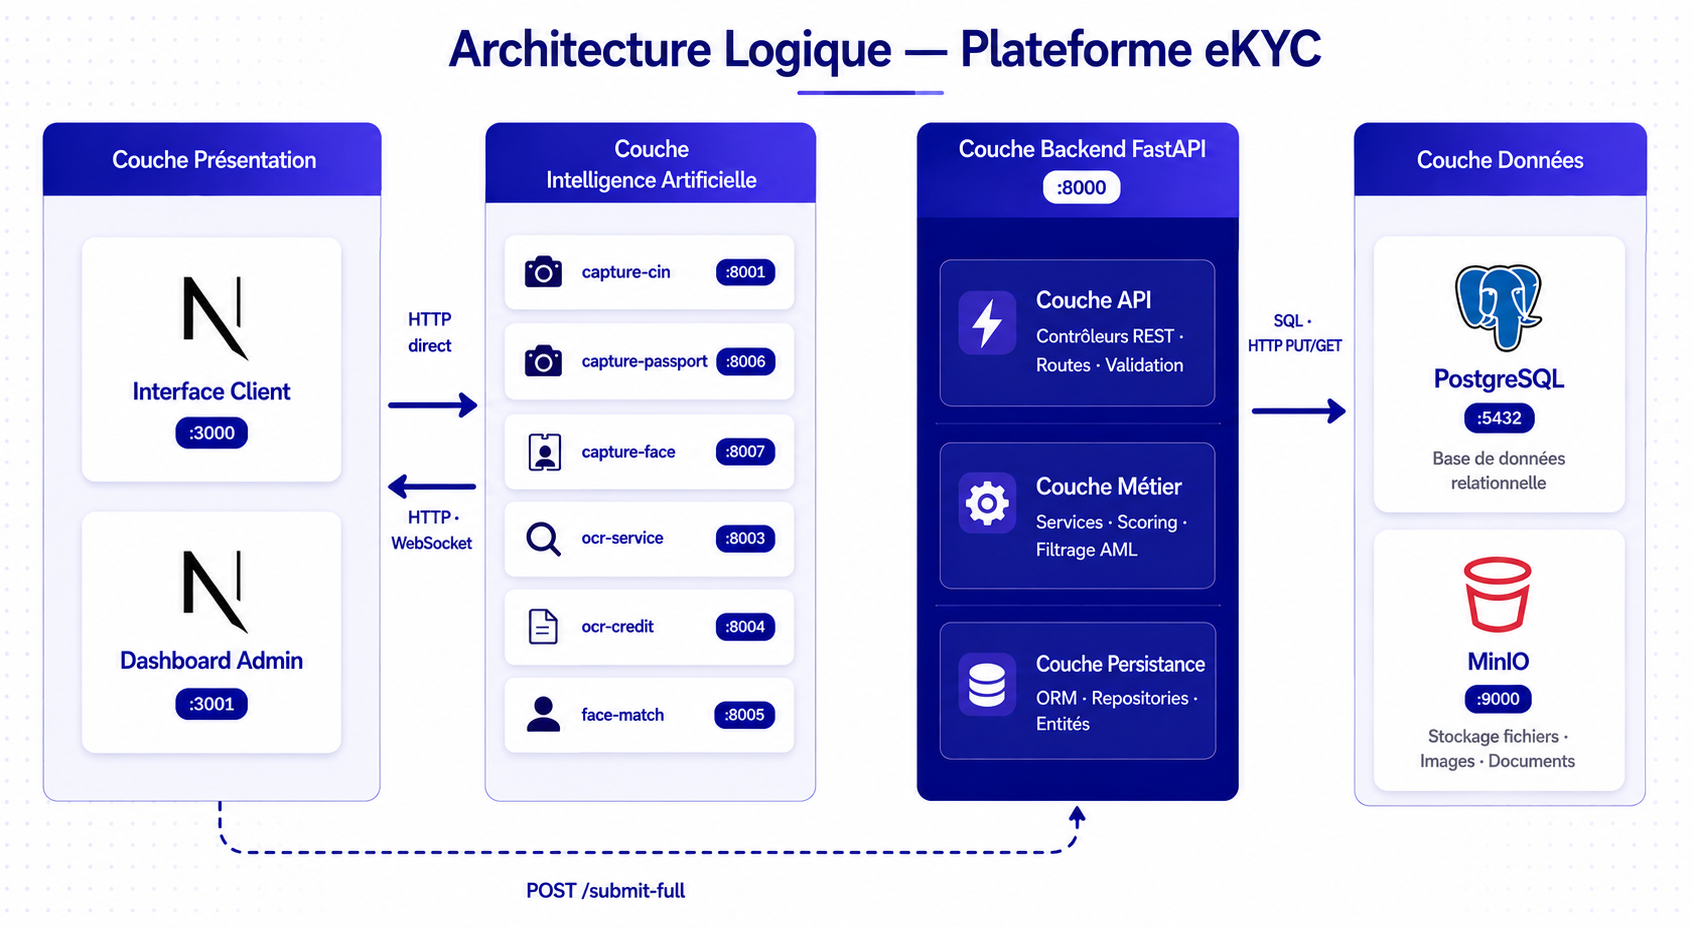
\includegraphics[width=0.95\textwidth]{images/architectures/logique.png}
  \captionof{figure}{Architecture logique de la plateforme eKYC}
  \label{fig:ch4-archi-logique}
\end{center}
\vspace{0.6em}

Cette organisation en quatre couches garantit une séparation claire des responsabilités. La vue physique ci-après précise comment ces couches se déploient concrètement sur l'infrastructure matérielle.

\subsection{Architecture physique}
\label{subsec:architecture-physique}

l'architecture physique de la plateforme eKYC, présentée dans la Figure~\ref{fig:ch4-archi-physique}, met en évidence les principaux éléments matériels et logiciels déployés ainsi que les échanges entre les postes clients, le serveur web, le serveur intelligence artificielle, le serveur backend et les serveurs de stockage. On y distingue les communications entre chaque composant : le poste client interagit avec le serveur web via HTTPS, le serveur web dialogue avec le serveur IA et le serveur backend, tandis que le serveur IA accède au stockage MinIO pour les images et le serveur backend persiste les données métier dans PostgreSQL.

\vspace{0.6em}
\begin{center}
  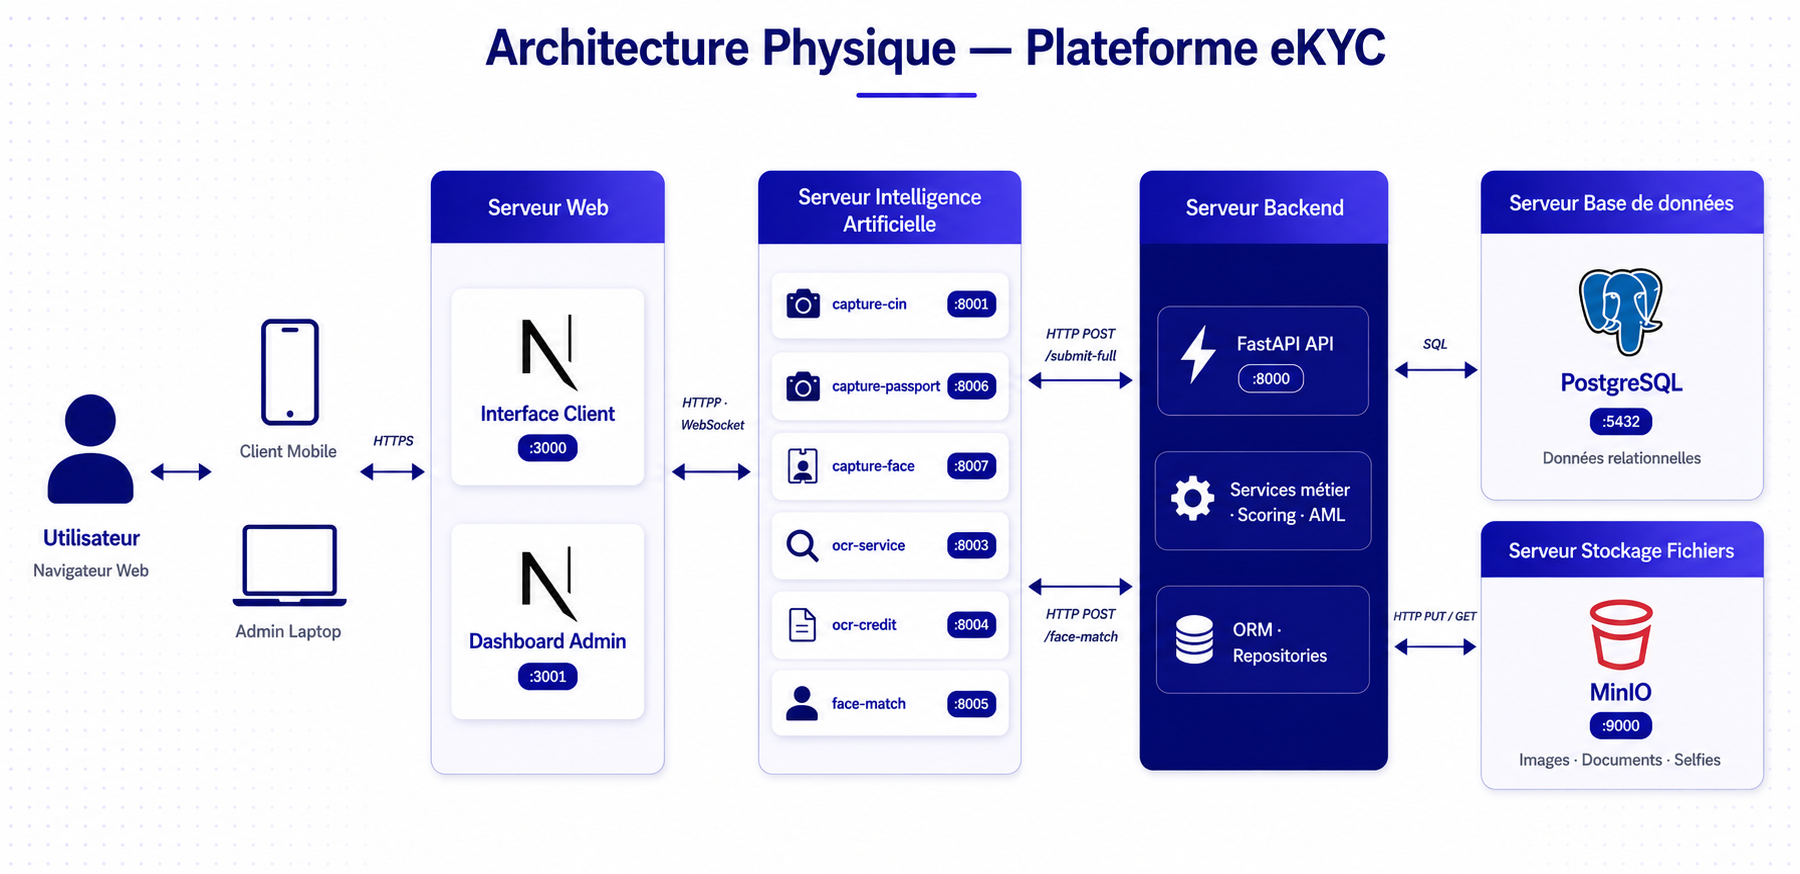
\includegraphics[width=0.95\textwidth]{images/architectures/physique.png}
  \captionof{figure}{Architecture physique de la plateforme eKYC}
  \label{fig:ch4-archi-physique}
\end{center}
\vspace{0.6em}

Les deux vues architecturales ainsi établies servent de base à la modélisation des interactions entre acteurs et système, formalisée dans la section suivante sous forme de diagrammes de cas d'utilisation.

%=============================================================
\section{Diagramme de cas d'utilisation global}
\label{sec:use-cases-global}
%=============================================================

Le diagramme de cas d'utilisation global illustrée par la Figure~\ref{fig:uc-global} offre une vue synthétique de l'ensemble des interactions entre les acteurs du système et la plateforme eKYC. Il met en évidence six profils d'acteurs aux périmètres fonctionnels distincts : le visiteur non inscrit, l'utilisateur authentifié engagé dans un parcours KYC, le client dont le compte est validé et qui accède aux services bancaires, l'analyste KYC chargé de statuer sur les dossiers, le responsable qualité IA qui surveille les performances des modèles, et l'administrateur qui hérite des droits des deux profils précédents tout en assurant la supervision globale de la plateforme.

\begin{figure}[H]
    \centering
    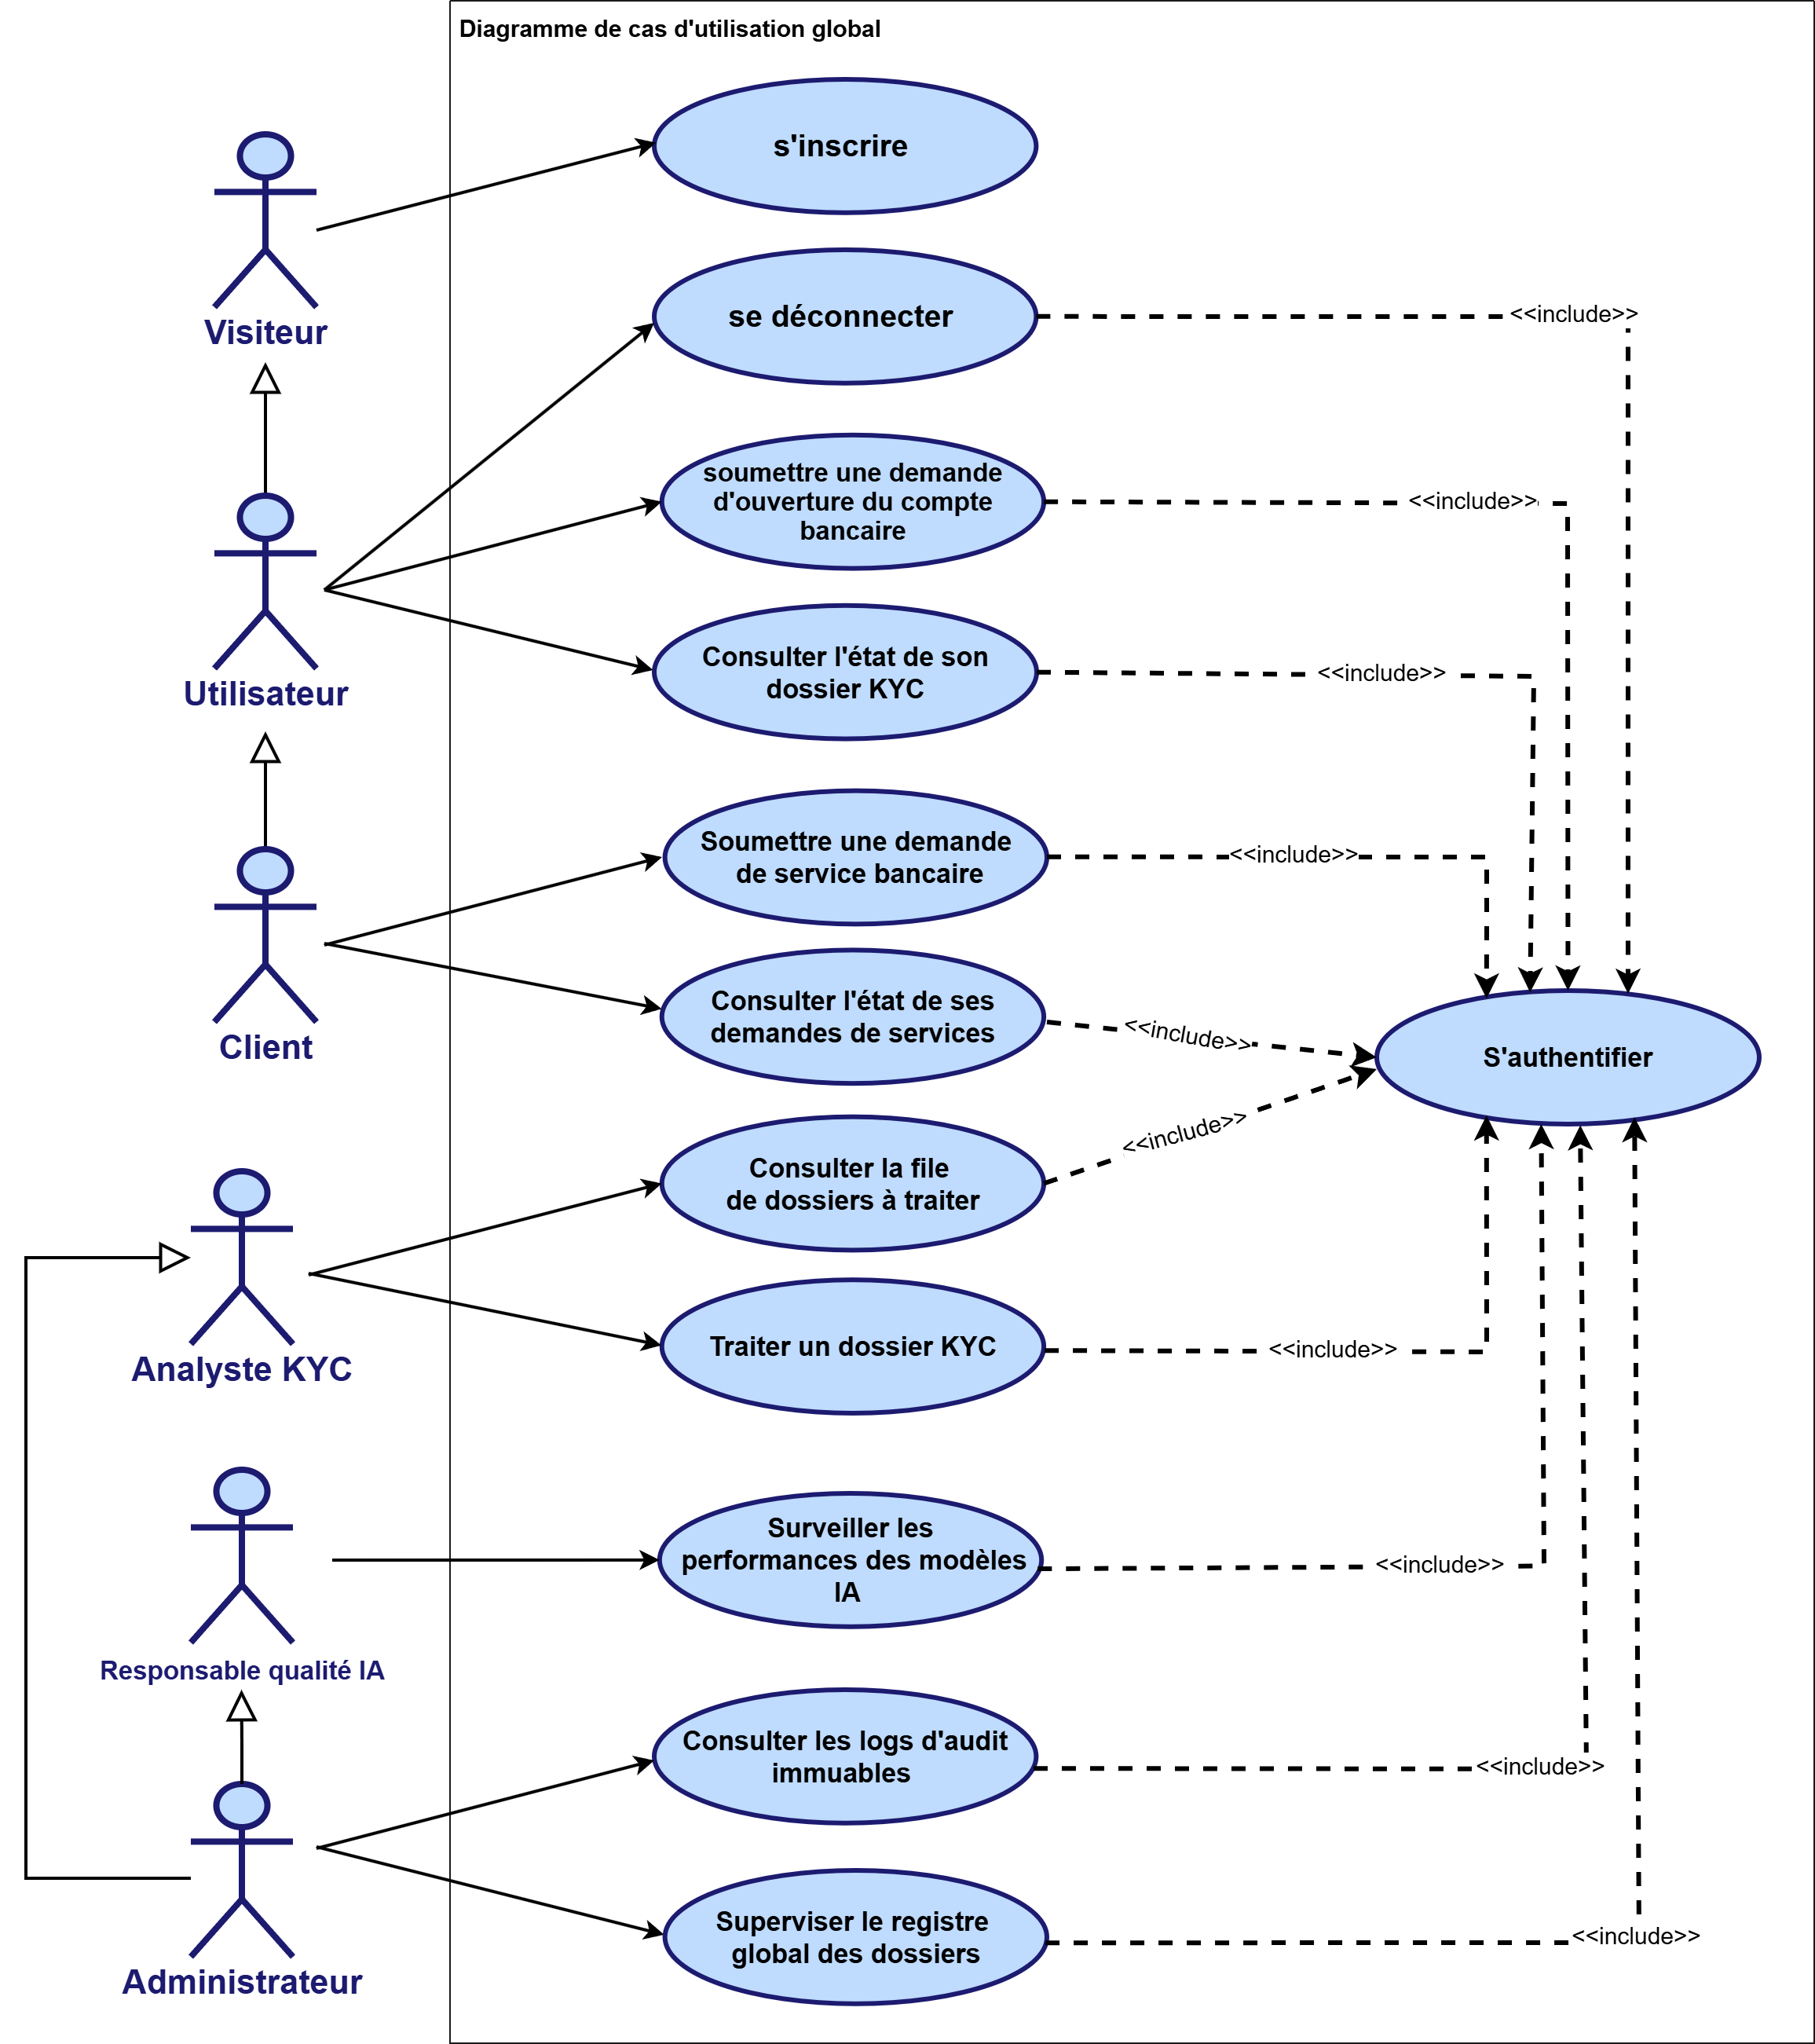
\includegraphics[width=\textwidth]{images/image_ch4/usecaseGlobale.png}
    \caption{Diagramme de cas d'utilisation global du système eKYC}
    \label{fig:uc-global}
\end{figure}

Ce diagramme constitue la vue d'ensemble des interactions du système. Les sous-sections suivantes détaillent chaque cas d'utilisation sous forme de tableaux structurés couvrant l'objectif, les préconditions, le scénario nominal et les alternatives.

%-------------------------------------------------------------
\subsection{Description des cas d'utilisation}
\label{subsec:description-uc}
%-------------------------------------------------------------

Les tableaux suivants décrivent de manière détaillée les principaux cas d'utilisation identifiés dans le diagramme global.

\renewcommand{\arraystretch}{1.5}

% ────────────────────────────────────────────────
% UC1 — S'inscrire
% ────────────────────────────────────────────────
\subsubsection{UC1 --- S'inscrire}

\begin{longtable}{|>{\bfseries}p{3.8cm}|p{10.2cm}|}
  \hline
  Cas d'utilisation    & S'inscrire (Création de compte) \\
  \hline
  Acteur principal     & Visiteur \\
  \hline
  Objectif             & Permettre à un visiteur de créer un compte sur l'interface client afin d'accéder au parcours KYC en utilisant son nom, son adresse électronique ou son numéro de téléphone et son mot de passe. \\
  \hline
  Préconditions        &
    - L'utilisateur ne possède pas encore de compte et accède à la page d'inscription. \newline
  \hline
  Scénario nominal     &
    - L'utilisateur accède au formulaire d'inscription de la plateforme. \newline
    - Il remplit le formulaire avec les informations requises : nom, adresse électronique ou numéro de téléphone et mot de passe. \newline
    - Le système valide les informations.\newline
    - Le système vérifie l'unicité de l'adresse électronique dans la base de données. \newline
    - Si toutes les informations sont valides, le compte est créé et un message de confirmation de création de compte est affiché. \newline
    - Le client est redirigé vers la page de connexion.. \\
  \hline
  Post-conditions      & Le compte de l'utilisateur est créé avec succès et enregistré dans la base de données. \\
  \hline
  Scénarios alternatifs &
    Le système affiche un message d'erreur et invite l'utilisateur à corriger les informations dans les cas suivants : \newline
    - Le format de l'adresse électronique est invalide ou le mot de passe est trop court. \newline
    - L'adresse électronique existe déjà dans la base de données (compte déjà existant). \\
  \hline
  \caption{UC1 --- S'inscrire}
  \label{tab:uc1}
\end{longtable}

Une fois le compte créé, l'utilisateur peut accéder à la plateforme via le mécanisme d'authentification décrit dans UC2.

% ────────────────────────────────────────────────
% UC2 — S'authentifier
% ────────────────────────────────────────────────
\subsubsection{UC2 --- S'authentifier}

\begin{longtable}{|>{\bfseries}p{3.8cm}|p{10.2cm}|}
  \hline
  Cas d'utilisation    & S'authentifier \\
  \hline
  Acteur principal     & Tout utilisateur disposant d'un compte (client, analyste KYC, responsable qualité IA, administrateur) \\
  \hline
  Objectif             & Accéder à l'espace personnel de la plateforme en présentant des identifiants valides. \\
  \hline
  Préconditions        &
    - L'utilisateur possède un compte actif sur la plateforme. \newline
    - L'utilisateur accède à la page de connexion. \\
  \hline
  Scénario nominal     &
    - L'utilisateur saisit son adresse électronique ou son numéro de téléphone(cas du client) et son mot de passe. \newline
    - Le système vérifie les identifiants et détermine le rôle associé au compte. \newline
    - L'utilisateur est redirigé vers l'interface correspondant à son profil (interface client, interface admin)\\
  \hline
  Post-conditions      & Une session sécurisée est ouverte. L'utilisateur accède aux fonctionnalités autorisées par son rôle. \\
  \hline
  Scénarios alternatifs &
    - Identifiants incorrects : le système affiche un message d'erreur générique sans préciser lequel des deux champs est erroné, par mesure de sécurité. \newline
    - Compte inexistant : l'utilisateur est invité à créer un compte ou à vérifier son adresse électronique. \\
  \hline
  \caption{UC2 --- S'authentifier}
  \label{tab:uc2}
\end{longtable}

Authentifié, l'utilisateur peut alors initier son parcours KYC, décrit dans UC3.

% ────────────────────────────────────────────────
% UC3 — Soumettre une demande KYC
% ────────────────────────────────────────────────
\subsubsection{UC3 --- Soumettre et suivre un dossier KYC}

\begin{longtable}{|>{\bfseries}p{3.8cm}|p{10.2cm}|}
  \hline
  Cas d'utilisation    & Soumettre et suivre un dossier KYC (parcours KYC) \\
  \hline
  Acteur principal     & Utilisateur authentifié \\
  \hline
  Objectif             & Déposer un dossier complet de demande d'ouverture de compte bancaire via un parcours guidé en quatre étapes, intégrant la capture du document d'identité, la vérification des données extraites, la capture du selfie biométrique et la soumission finale. \\
  \hline
  Préconditions        &
    - L'utilisateur est authentifié sur la plateforme. \newline
    - Il dispose d'un document d'identité valide (carte d'identité nationale ou passeport) et d'un accès à la caméra de son appareil. \\
  \hline
  Scénario nominal     &
    \textbf{Étape 1 : Capture du document d'identité.} L'utilisateur choisit le type de document (carte d'identité nationale en deux captures recto/verso, ou passeport en une seule capture). La caméra s'ouvre avec un cadre guide adapté. Le système analyse chaque image en temps réel~; le bouton de capture est initialement désactivé et ne s'active que lorsque le service IA confirme que le document détecté est valide (CIN ou passeport reconnu). L'utilisateur déclenche alors manuellement la capture. L'extraction des données textuelles est déclenchée en arrière-plan. \newline\newline
    \textbf{Étape 2 : Vérification des informations extraites.} L'utilisateur consulte les données extraites depuis son document. Il peut corriger manuellement tout champ inexact ; chaque correction est enregistrée et transmise à l'analyste KYC. \newline\newline
    \textbf{Étape 3 : Capture du selfie .} La caméra s'ouvre avec un cadre ovale centré. Le système détecte le visage en temps réel et active la capture dès que le cadrage est satisfaisant. \newline\newline
    \textbf{Étape 4 : Récapitulatif et soumission finale.} L'utilisateur vérifie l'ensemble des informations collectées, coche les cases de consentement et soumet sa demande. Le dossier complet est enregistré en base de données avec le statut « en attente » et un numéro de référence est communiqué à l'utilisateur. \\
  \hline
  Post-conditions      & Un dossier KYC complet est créé avec le statut « en attente ». L'utilisateur peut suivre l'évolution de son dossier depuis son espace personnel. \\
  \hline
  Scénarios alternatifs &
    - Document non reconnu : le système invite l'utilisateur à recommencer la capture dans de meilleures conditions d'éclairage. \newline
    - Selfie non conforme : l'utilisateur est invité à recommencer la capture en respectant les consignes de positionnement. \newline
    - Échec de soumission : les données restent conservées localement et l'utilisateur peut relancer la soumission. \\
  \hline
  \caption{UC3 --- Soumettre une demande d'ouverture de compte bancaire}
  \label{tab:uc3}
\end{longtable}

Une fois le dossier soumis par le client, il entre dans la file de traitement de l'analyste KYC, dont les actions sont formalisées dans UC4.

% ────────────────────────────────────────────────
% UC4 — Traiter un dossier KYC
% ────────────────────────────────────────────────
\subsubsection{UC4 --- Traiter un dossier KYC}

\begin{longtable}{|>{\bfseries}p{3.8cm}|p{10.2cm}|}
  \hline
  Cas d'utilisation    & Traiter un dossier KYC \\
  \hline
  Acteur principal     & Analyste KYC (ou Administrateur) \\
  \hline
  Objectif             & Examiner un dossier de demande d'ouverture de compte, vérifier la conformité des données et des documents soumis, et prendre une décision sur la suite à donner à la demande. \\
  \hline
  Préconditions        &
    - L'analyste est authentifié avec le rôle approprié. \newline
    - Au moins un dossier KYC est en attente de traitement dans la file. \\
  \hline
  Scénario nominal     &
    - L'analyste consulte la file d'attente des dossiers triée par ordre d'ancienneté et sélectionne un dossier à instruire. \newline
    - Il accède à la page de revue complète : images des documents, données extraites, corrections apportées par le client et résultat de la comparaison biométrique. \newline
    - Il vérifie les données extraites et corrige si nécessaire tout champ erroné. Chaque correction est horodatée et invalide les résultats de filtrage précédemment calculés. \newline
    - Le système présente les résultats de la vérification de conformité documentaire (cohérence des champs obligatoires, validité de la date d'expiration) et calcule un score de conformité. \newline
    - L'analyste lance le filtrage anti-blanchiment, qui confronte les données du client à la liste des personnes blacklistées, à la liste des personnes politiquement exposées et à la base des dossiers validés pour détecter d'éventuels doublons d'identité. \newline
    - L'analyste consulte le score de risque global agrégeant les résultats du filtrage, la conformité documentaire et la similarité biométrique. Le système formule une recommandation automatique. \newline
    - L'analyste prend sa décision finale : approbation, rejet motivé ou demande de complément documentaire. La décision est enregistrée et le client est notifié. \\
  \hline
  Post-conditions      & Le dossier est mis à jour avec la décision de l'analyste. Si approuvé, le compte bancaire est activé. Si rejeté, le motif est transmis au client. \\
  \hline
  Scénarios alternatifs &
    - Alerte AML confirmée : si l'alerte est avérée, la demande est rejetée ; si elle est écartée, le score de risque est recalculé en excluant cette alerte. \newline
    - Documents insuffisants : l'analyste sélectionne le statut « incomplet » et précise les pièces manquantes. \newline
    - Discordance biométrique : l'analyste peut rejeter la demande ou solliciter un complément d'information auprès du client. \\
  \hline
  \caption{UC4 --- Traiter un dossier KYC}
  \label{tab:uc4}
\end{longtable}

En parallèle du traitement des dossiers, le responsable qualité IA assure la supervision continue des modèles via UC5.

% ────────────────────────────────────────────────
% UC5 — Surveiller les performances des modèles IA
% ────────────────────────────────────────────────
\subsubsection{UC5 --- Surveiller les performances des modèles IA}

\begin{longtable}{|>{\bfseries}p{3.8cm}|p{10.2cm}|}
  \hline
  Cas d'utilisation    & Surveiller les performances des modèles IA \\
  \hline
  Acteur principal     & Responsable qualité IA (ou Administrateur) \\
  \hline
  Objectif             & Évaluer en continu la qualité des traitements automatiques produits par les modèles de détection et d'extraction, afin de détecter toute dégradation de performance et d'orienter les actions correctives. \\
  \hline
  Préconditions        &
    - Le responsable est authentifié avec le rôle approprié. \newline
    - Des dossiers ont été traités par le système, générant des données de performance exploitables. \\
  \hline
  Scénario nominal     &
    - Le responsable accède à la page de supervision IA et sélectionne le type de document à analyser (carte d'identité recto, verso ou passeport) ainsi que la période d'observation. \newline
    - Il consulte les indicateurs clés de performance globaux : précision, rappel, score F1 et latence moyenne pour le pipeline complet et pour chacun des deux modèles séparément. \newline
    - Il examine le graphique d'évolution hebdomadaire des scores de confiance pour détecter toute tendance à la dégradation dans le temps. \newline
    - Il analyse les performances du modèle de détection champ par champ : score de confiance moyen, taux de zones manquantes et taux de faux positifs. \newline
    - Il analyse les performances du moteur de lecture champ par champ : score de confiance OCR moyen, taux de corrections manuelles et taux de champs vides. \newline
    - Il consulte le graphique de corrélation entre les scores des deux modèles pour identifier les zones présentant une incohérence. \newline
    - En cas d'anomalie, il documente ses observations et déclenche une action corrective sur le modèle ou le prétraitement concerné. \\
  \hline
  Post-conditions      & Le responsable dispose d'une vue objective et actualisée de la qualité des traitements. Les anomalies identifiées sont documentées et transmises aux équipes techniques. \\
  \hline
  Scénarios alternatifs &
    - Dégradation détectée : un signal d'alerte visuel est affiché lorsqu'un indicateur passe sous le seuil de qualité cible (ex. taux de correction dépassant 10\,\% sur un champ). \newline
    - Aucune donnée disponible : la page affiche un message informatif et invite à élargir la fenêtre temporelle d'observation. \\
  \hline
  \caption{UC5 --- Surveiller les performances des modèles IA}
  \label{tab:uc5}
\end{longtable}
\section*{Conclusion du chapitre}

Ce chapitre a établi le référentiel complet de la plateforme eKYC : identification des quatre profils d'acteurs, formalisation des besoins fonctionnels couvrant l'ensemble du parcours client et des fonctions d'administration, et définition des contraintes non fonctionnelles en matière de sécurité, de confidentialité, de conformité réglementaire et de performance. L'architecture logique et physique retenue traduit ces exigences en une organisation modulaire et souveraine, tandis que les diagrammes de cas d'utilisation en formalisent les interactions. Ces éléments constituent le socle sur lequel s'appuient la conception détaillée et la réalisation présentées dans les chapitres suivants.


% ============================================================
% PARTIE I
% ============================================================

\addcontentsline{toc}{part}{Incrément 1 : Fondements IA et Réalisation du Pipeline}
\pagepartie{I}{Incrément 1 : Fondements IA\\[0.4em]et Réalisation du Pipeline}

% ============================================================
% CHAPITRE 3
% ============================================================

\chapter{Fondements Théoriques et Choix Technologiques}
\label{chap:fondements-techniques}

La mise en œuvre d'un système d'automatisation du processus KYC repose sur un socle théorique et technologique solide. Ce chapitre pose les bases conceptuelles nécessaires à la compréhension des choix effectués, depuis les fondements de l'intelligence artificielle et de la vision par ordinateur jusqu'aux technologies retenues. Une fois ce cadre établi, il devient possible de justifier rigoureusement la sélection des outils constituant le pipeline IA du projet.


%=============================================================
\section{Fondements théoriques}
\label{sec:fondements-theoriques}
%=============================================================

\subsection{Intelligence artificielle, machine learning et deep learning}
\label{subsec:ia-ml-dl}

Avant d'aborder la vision par ordinateur, il convient de présenter la hiérarchie conceptuelle sur laquelle elle repose. Ces trois disciplines s'emboîtent selon une relation de spécialisation croissante, chacune constituant un sous-ensemble plus restreint de la précédente.

\begin{figure}[H]
  \centering
  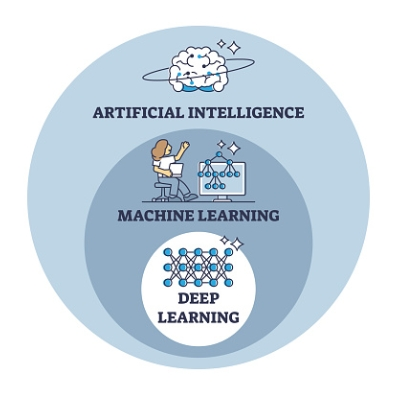
\includegraphics[width=0.75\textwidth]{images/image_chap2/ia_ml_dl.png}
  \caption{\textit{Figure 2.1 --- Relation hiérarchique entre IA, ML et Deep Learning}}
  \label{fig:ch2-ia-ml-dl}
\end{figure}

\begin{itemize}
  \item \textbf{Intelligence Artificielle (IA) :} domaine regroupant l'ensemble des techniques permettant à une machine de simuler des comportements intelligents --- apprentissage, raisonnement et prise de décision.

  \item \textbf{Machine Learning (ML) :} sous-discipline de l'IA dans laquelle les systèmes apprennent à partir de données, sans être explicitement programmés pour chaque tâche.

  \item \textbf{Deep Learning (DL) :} évolution du ML fondée sur des réseaux de neurones profonds, capables de traiter des données complexes (images, audio, texte). Le Deep Learning constitue aujourd'hui le moteur principal des systèmes de vision par ordinateur.
\end{itemize}

\subsection{Vision par ordinateur et réseaux de neurones}
\label{subsec:vision-ordinateur}

La vision par ordinateur est une branche de l'intelligence artificielle qui permet aux machines d'interpréter et de comprendre le contenu visuel d'images ou de vidéos. Son objectif est de transformer des données visuelles brutes --- des pixels --- en informations sémantiques exploitables, reproduisant ainsi de façon automatisée les capacités du système visuel humain.

Dans le cadre du KYC, la vision par ordinateur intervient à travers plusieurs applications complémentaires et étroitement liées :

\begin{itemize}
  \item \textbf{Reconnaissance d'images :} identification du type de document (carte nationale d'identité, passeport, etc.).

  \item \textbf{Détection d'objets :} localisation des zones d'intérêt --- photographie, champs textuels.

  \item \textbf{Reconnaissance optique de caractères (OCR) :} extraction et conversion du texte présent dans l'image en données numériques structurées.
\end{itemize}

Ces applications reposent sur les réseaux de neurones artificiels, brique fondamentale du Deep Learning. Inspirés du fonctionnement du cortex cérébral, ces réseaux sont composés de neurones interconnectés organisés en couches successives, chacune apprenant à extraire des représentations de plus en plus abstraites à partir des données d'entrée.

\begin{figure}[H]
  \centering
  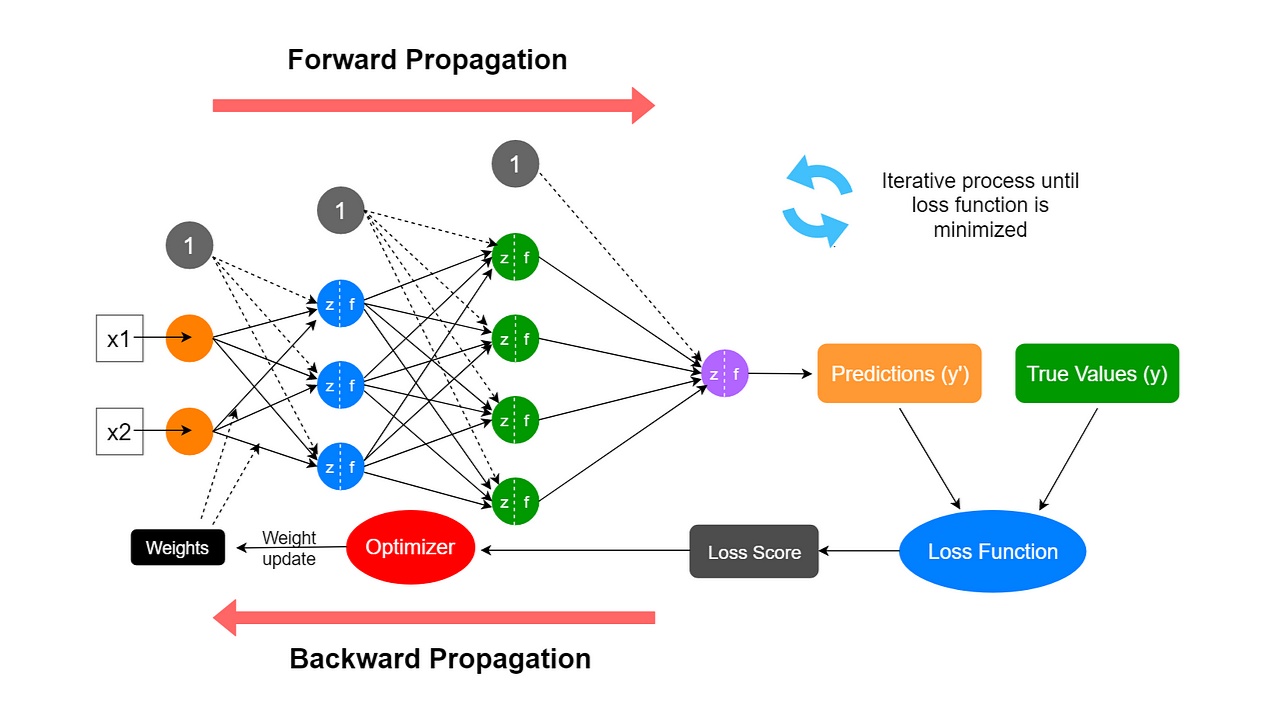
\includegraphics[width=0.75\textwidth]{images/image_chap2/1742401020360.png}
  \caption{\textit{Figure 2.2 --- Propagation avant et rétropropagation dans un réseau de neurones}}
  \label{fig:ch2-neurones}
\end{figure}

L'architecture d'un réseau de neurones se décompose en trois types de couches :

\begin{itemize}
  \item \textbf{Couche d'entrée (Input Layer) :} reçoit les données brutes --- pixels de l'image du document --- et les transmet aux couches suivantes.

  \item \textbf{Couches cachées (Hidden Layers) :} traitent l'information à travers plusieurs étapes de calcul afin d'extraire les caractéristiques complexes (contours, formes, zones de texte).

  \item \textbf{Couche de sortie (Output Layer) :} fournit la prédiction finale, telle que la probabilité qu'une zone détectée corresponde à un nom, un prénom ou un numéro de CIN.
\end{itemize}

Le fonctionnement repose sur deux phases complémentaires et itératives :

\begin{itemize}
  \item \textbf{Propagation avant (Forward Propagation) :} l'information circule de l'entrée vers la sortie pour générer une prédiction, en appliquant des poids et des biais à chaque neurone.

  \item \textbf{Rétropropagation (Backpropagation) :} le système calcule l'erreur via une fonction de perte et remonte le réseau pour ajuster les poids grâce à un optimiseur, permettant au modèle d'apprendre de ses erreurs de manière itérative.
\end{itemize}

\subsection{Détection d'objets}
\label{subsec:detection-objets}

La détection d'objets est une tâche centrale de la vision par ordinateur qui consiste à identifier et localiser simultanément plusieurs objets dans une image ou une vidéo. Contrairement à la classification d'images --- qui attribue une unique étiquette à l'ensemble de l'image --- la détection d'objets détermine la position précise de chaque objet à l'aide de boîtes englobantes (bounding boxes).

\begin{figure}[H]
  \centering
  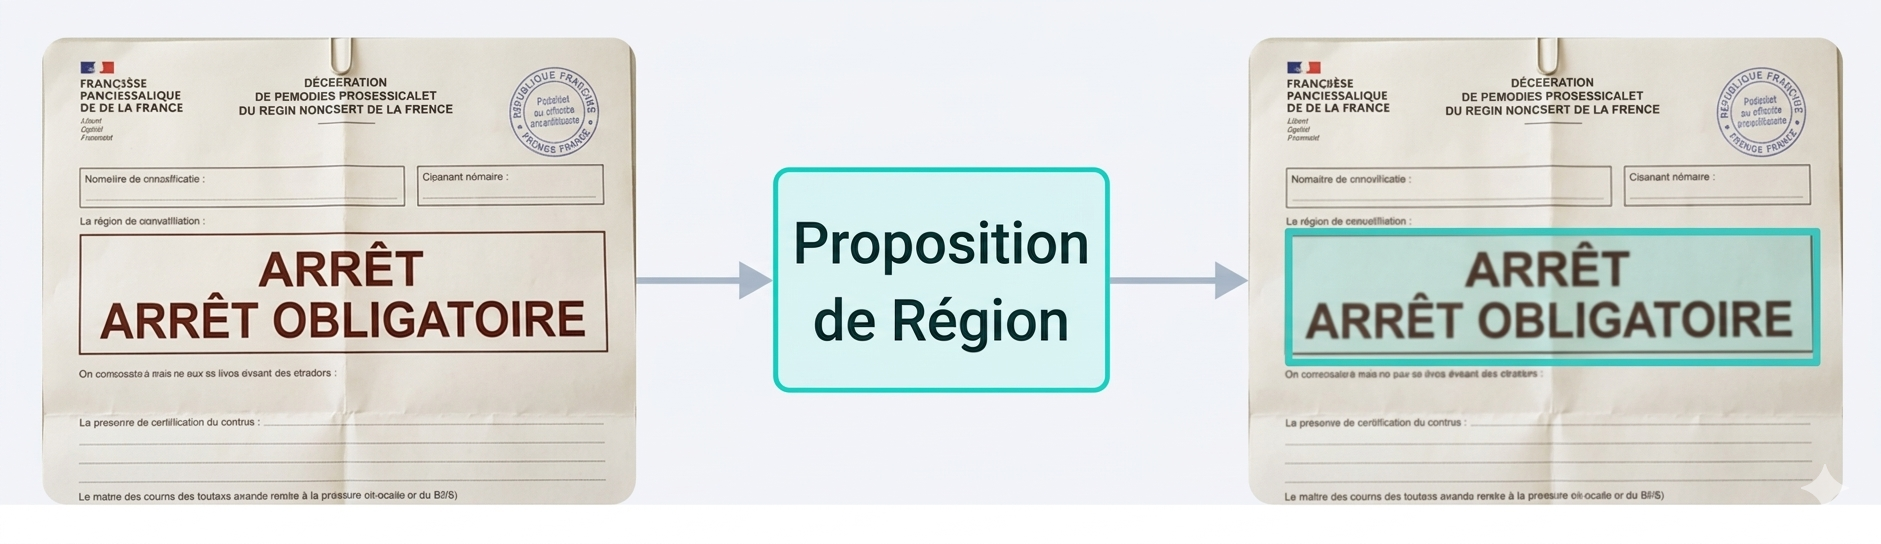
\includegraphics[width=0.75\textwidth]{images/image_chap2/detectionObjet.png}
  \caption{\textit{Figure 2.3 --- Illustration de la détection d'objets}}
  \label{fig:ch2-detection-objets}
\end{figure}

\subsubsection*{Niveaux de complexité des tâches de vision}

Pour bien situer la détection d'objets dans le spectre des tâches de vision par ordinateur, il est utile de les classer par ordre de complexité croissante :

\begin{itemize}
  \item \textbf{Classification d'image :} prédire la classe d'un objet unique dans l'image (ex. : « Ceci est une carte d'identité »).

  \item \textbf{Localisation d'objet :} identifier la présence d'un objet et indiquer sa position par une boîte englobante.

  \item \textbf{Détection d'objets :} identifier et localiser plusieurs objets et leurs classes respectives dans une même image.

  \item \textbf{Segmentation sémantique :} classifier chaque pixel de l'image dans une catégorie, sans distinguer les différentes instances d'une même classe.

  \item \textbf{Segmentation d'instance :} identifier et délimiter chaque objet distinct --- par exemple, séparer deux cartes d'identité disposées côte à côte.
\end{itemize}

\subsubsection*{Méthodes de détection : One-Stage vs Two-Stage}

Les méthodes de détection d'objets basées sur le Deep Learning se répartissent en deux grandes familles architecturales, dont le choix est guidé par le compromis entre vitesse d'inférence et précision.

\begin{figure}[H]
  \centering
  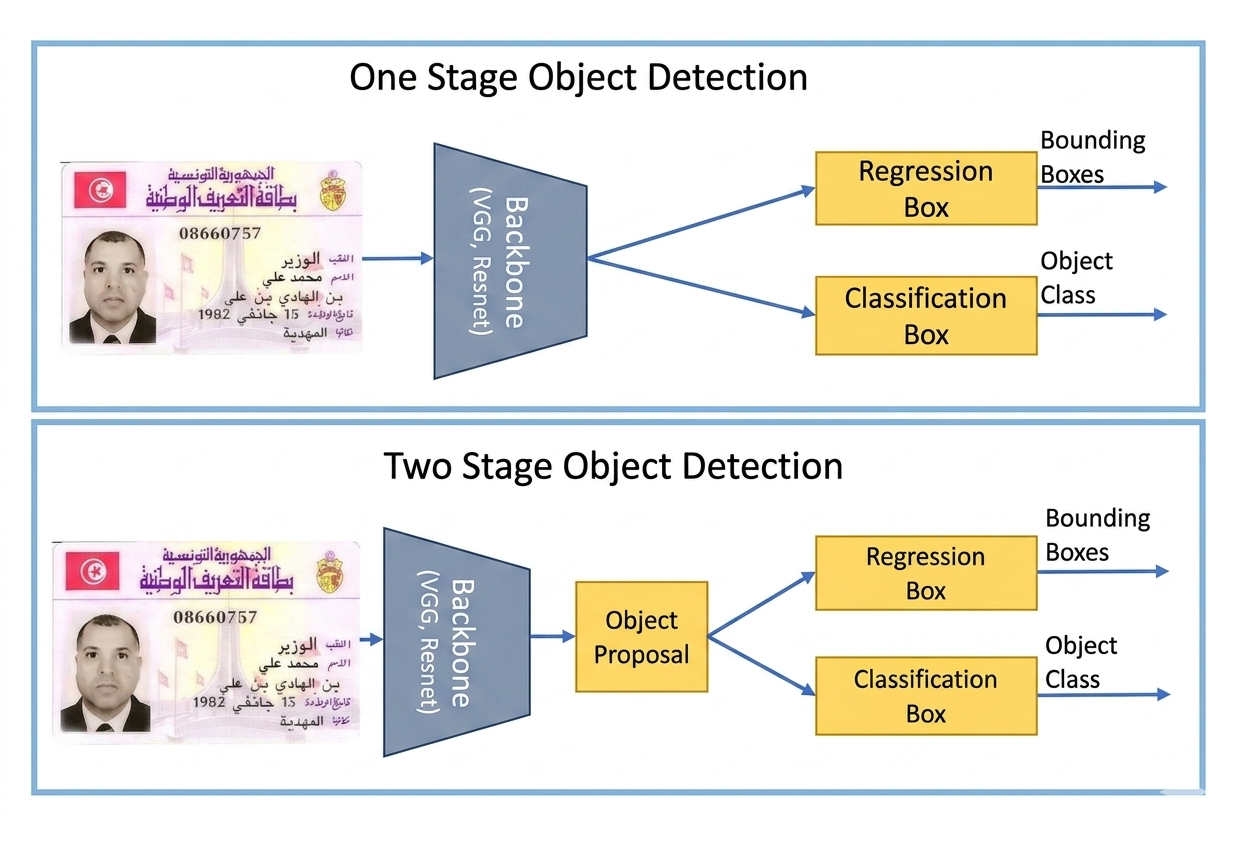
\includegraphics[width=0.45\textwidth]{images/image_chap2/onevtwoStage.png}
  \caption{\textit{Méthodes de détection d'objets : One-Stage vs Two-Stage}}
  \label{fig:ch2-one-vs-two-stage}
\end{figure}

\paragraph{Méthodes One-Stage}

Ces méthodes utilisent un réseau unique qui mappe directement l'image d'entrée vers les prédictions (boîtes englobantes et classes) en un seul passage. Leur architecture simplifiée leur confère une vitesse d'inférence élevée, idéale pour les applications en temps réel (vidéo, mobile). Exemples représentatifs : YOLO, SSD.

\paragraph{Méthodes Two-Stage}

Elles procèdent en deux étapes distinctes : une première génère des propositions de régions d'intérêt (Region Proposals), et une seconde affine et classifie ces propositions. Leur précision est généralement supérieure, au prix d'une latence plus élevée et d'un coût computationnel important. Exemples : Faster R-CNN, R-CNN.

\subsubsection*{YOLO (You Only Look Once)}

\begin{figure}[H]
  \centering
  
\includegraphics[width=0.45\textwidth]{images/image_chap2/yoloLogo.png}
  \caption{\textit{Figure 2.5 --- Logo YOLO}}
  \label{fig:ch2-yolo-logo}
\end{figure}

YOLO (You Only Look Once) est un algorithme de détection d'objets appartenant à la famille One-Stage, introduit en 2016 par Joseph Redmon et ses collaborateurs. Ce modèle a révolutionné la détection d'objets en proposant une approche unifiée, capable de détecter et classifier des objets en un seul passage réseau, atteignant des performances en temps réel tout en conservant une précision compétitive.

\paragraph{Principe de fonctionnement}
\begin{figure}[H]
  \centering
  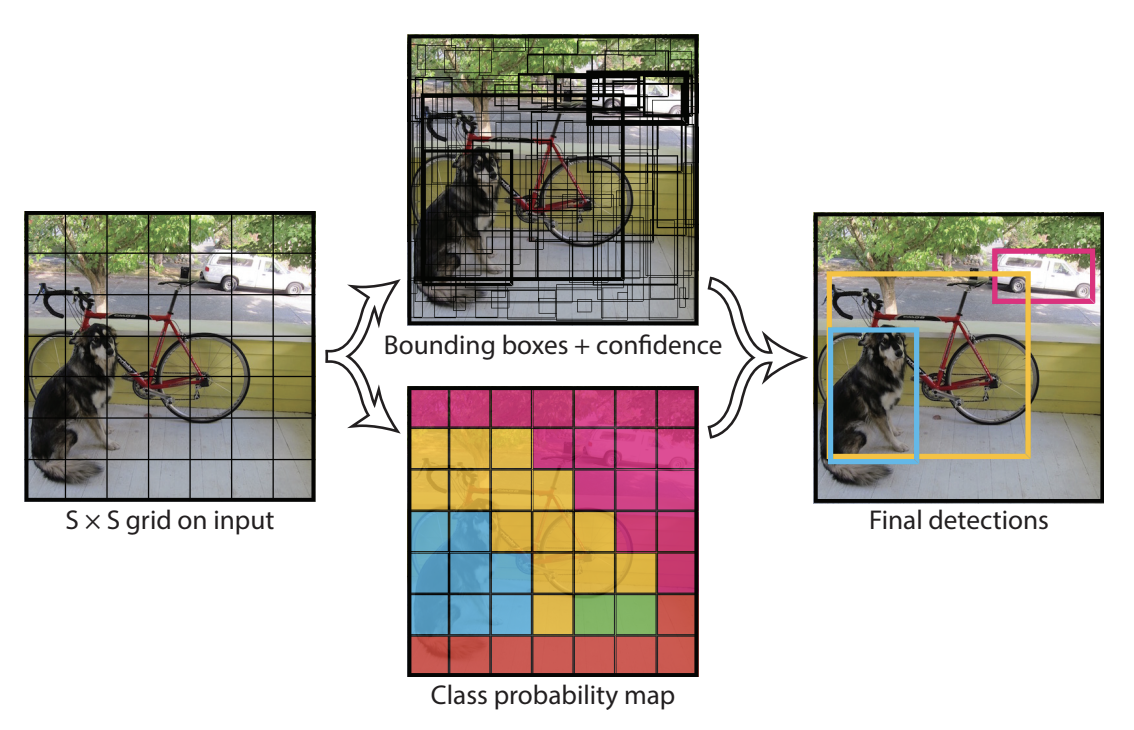
\includegraphics[width=0.75\textwidth]{images/image_chap2/detection.png}
  \caption{\textit{Principe de fonctionnement de YOLO}}
  \label{fig:Principe de fonctionnement de YOLO }
\end{figure}

Comme illustré ci-après, YOLO adopte une approche globale et unifiée :

\begin{itemize}
  \item L'image est divisée en une grille de cellules $S \times S$.
  \item Chaque cellule est responsable de la détection des objets dont le centre se situe dans sa zone.
  \item Pour chaque cellule, le modèle prédit simultanément : des boîtes englobantes, un score de confiance et la classe de l'objet.
  \item L'ensemble de ces prédictions est réalisé en un seul passage à travers le réseau, garantissant rapidité et efficacité.
\end{itemize}

\paragraph{Évolution de l'architecture YOLO}

Depuis l'introduction de YOLOv1, le modèle a connu de nombreuses itérations, chacune améliorant la précédente en termes de précision, de rapidité et d'efficacité.

\begin{figure}[H]
  \centering
  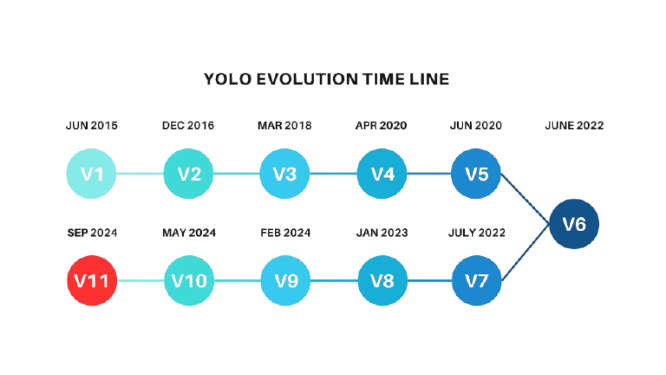
\includegraphics[width=0.90\textwidth]{images/image_chap2/TimelineCycle-removebg-preview.png}
  \caption{\textit{Figure 2.6 --- Chronologie de l'évolution des architectures YOLO (V1 à V11)}}
  \label{fig:ch2-yolo-evolution}
\end{figure}

\begin{itemize}
  \item \textbf{YOLOv1 (2016) :} modèle original --- performances temps réel, mais détection des petits objets limitée.

  \item \textbf{YOLOv2 (2017) :} introduction des boîtes d'ancrage, normalisation par lots et résolution accrue.

  \item \textbf{YOLOv3 (2018) :} prédictions multi-échelles via pyramides de features, améliorant la détection à différentes tailles d'objets.

  \item \textbf{YOLOv4 (2020) :} augmentation mosaïque et optimisation du backbone pour une inférence plus rapide.

  \item \textbf{YOLOv5 (2020) :} implémentation PyTorch largement adoptée, optimisée pour le déploiement pratique.

  \item \textbf{YOLOv6/v7 (2022) :} amélioration de la mise à l'échelle et de la précision, avec des versions compactes pour edge devices.

  \item \textbf{YOLOv8 (2023) :} backbone CSPDarkNet et agrégation de chemins améliorée, rehaussant vitesse et précision.

  \item \textbf{YOLO11 (2024) :} architecture C3K2 + SPPF + mécanisme d'attention C2PSA --- meilleure détection des petits objets et efficacité computationnelle supérieure.
\end{itemize}

\paragraph{Analyse comparative sur COCO}

\begin{figure}[H]
  \centering
  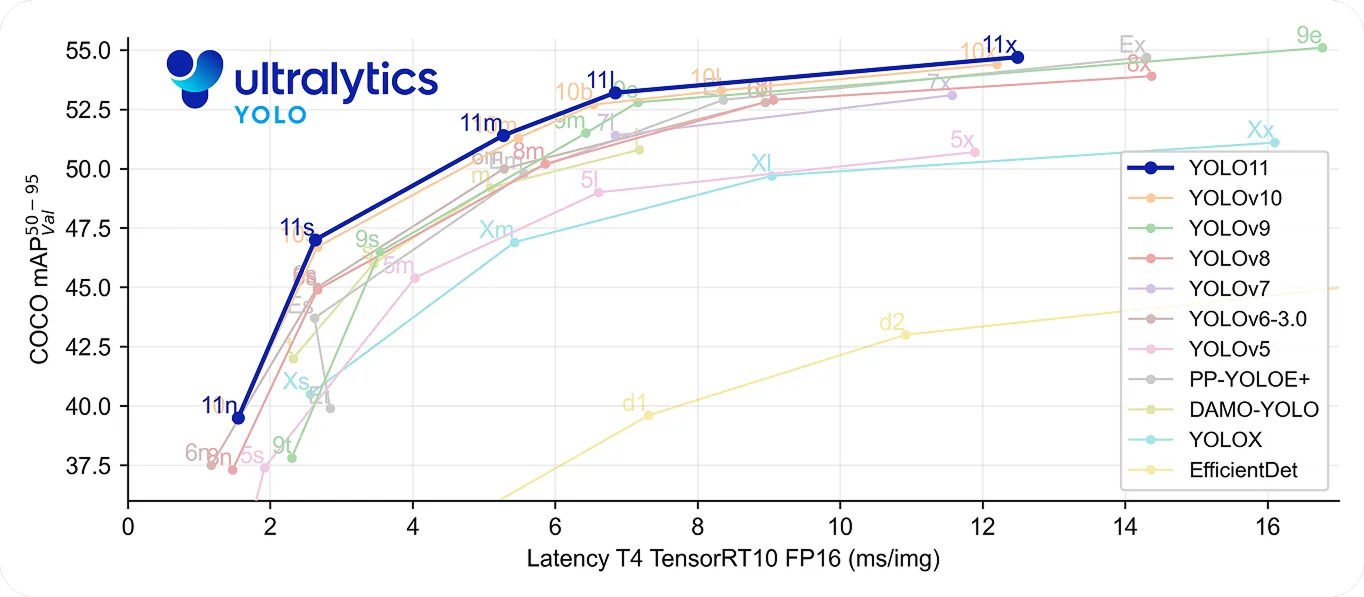
\includegraphics[width=0.75\textwidth]{images/image_chap2/Latency.png}
  \caption{\textit{Comparaison mAP50-95 / latence des modèles YOLO sur le dataset COCO}}
  \label{fig:ch2-yolo-comparaison}
\end{figure}

La figure ci-dessus compare les modèles YOLO à l'aide de la métrique mAP50-95 (mean Average Precision) sur le dataset COCO, en fonction de leur latence d'inférence. Les versions récentes offrent de meilleures performances, avec une précision accrue et une latence réduite. YOLO11 se distingue notamment par son efficacité : plus léger que ses homologues à haute précision, il conserve un excellent niveau de mAP, le rendant particulièrement adapté aux applications en temps réel.

\subsection{Reconnaissance optique de caractères (OCR)}
\label{subsec:ocr}

La reconnaissance optique de caractères (OCR --- Optical Character Recognition) est une technologie permettant d'extraire automatiquement du texte à partir d'images ou de documents numérisés. Elle transforme des informations textuelles visuelles en données numériques exploitables, facilitant leur traitement, leur stockage et leur analyse automatisée.

Dans le cadre des systèmes KYC, l'OCR joue un rôle central en permettant d'extraire les informations présentes sur les documents d'identité : nom, prénom, date de naissance, numéro d'identification, etc.

\subsubsection*{Pipeline OCR : processus pas à pas}

Le pipeline OCR se compose de cinq étapes séquentielles qui transforment une image brute en texte structuré exploitable :

\begin{figure}[H]
  \centering
  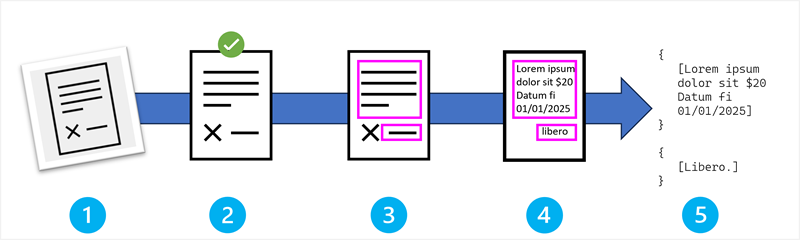
\includegraphics[width=0.75\textwidth]{images/image_chap2/optical-character-recognition.png}
  \caption{\textit{Figure 2.8 --- Pipeline OCR en cinq étapes}}
  \label{fig:ch2-ocr-pipeline}
\end{figure}

\begin{itemize}
  \item \textbf{Étape 1 --- Acquisition et entrée d'image :} le pipeline démarre à la réception de l'image. La qualité de celle-ci conditionne directement la précision finale de l'extraction de texte.

  \item \textbf{Étape 2 --- Prétraitement et amélioration :} nettoyage et optimisation de l'image pour améliorer la lisibilité.

  \item \textbf{Étape 3 --- Détection des régions textuelles :} localisation des zones contenant du texte au sein de l'image.

  \item \textbf{Étape 4 --- Reconnaissance des caractères :} identification des caractères présents dans les zones détectées.

  \item \textbf{Étape 5 --- Post-traitement et sortie :} structuration et correction des données extraites.
\end{itemize}

Ce processus permet de transformer une image contenant du texte en un format exploitable par un système informatique.

\subsubsection*{Benchmark des moteurs OCR open source}

Plusieurs solutions OCR open source ont été développées, présentant des performances variables en termes de précision, de robustesse et de vitesse. Les approches basées sur le Deep Learning, telles que PaddleOCR, se révèlent généralement plus performantes en conditions réelles (flou, bruit, faible éclairage), ce qui les rend particulièrement adaptées aux systèmes KYC.

\begin{table}[H]
  \centering
  \tiny
  \begin{tabular}{|l|c|c|c|c|c|c|c|}
    \toprule
    \rowcolor{bleu_principal}
    \textcolor{white}{\textbf{Moteur}} & \textcolor{white}{\textbf{Archi.}} & \textcolor{white}{\textbf{Préc.}} & \textcolor{white}{\textbf{CER}} & \textcolor{white}{\textbf{Vit.}} & \textcolor{white}{\textbf{Ar.}} & \textcolor{white}{\textbf{FT}} & \textcolor{white}{\textbf{Lic.}} \\
    \midrule
    Tesseract & LSTM + HMM & ~90\% & 3--5\% & Très rapide & Oui & Oui & Apache 2.0 \\
    \midrule
    \rowcolor{gris_leger}
    PaddleOCR & CNN + Transformer & ~93\% & 2--4\% & Moyen & Oui & Oui & Apache 2.0 \\
    \midrule
    EasyOCR & CRAFT + CRNN & ~85\% & 5--8\% & Lent & Oui & Partiel & Apache 2.0 \\
    \midrule
    \rowcolor{gris_leger}
    Kraken v5 & BLLA + CLSTM & ~82\% & 2--5\% & Rapide & Excellent RTL & Oui & Apache 2.0 \\
    \midrule
    MMOCR v1 & CNN / Transformer & ~84\% & 4--7\% & Moyen & Partiel & Oui & Apache 2.0 \\
    \midrule
    \rowcolor{gris_leger}
    TrOCR & ViT + BEiT & ~91\% & 2--4\% & Lent (GPU) & Non off. & Oui & MIT \\
    \bottomrule
  \end{tabular}
  \caption{Benchmark des principaux moteurs OCR open source (mise à jour 2025)}
  \label{tab:ocr-benchmark}
\end{table}

Les scores de précision sont des moyennes indicatives sur texte imprimé propre (300 DPI+). Le CER (Character Error Rate) varie significativement selon la qualité du scan, la langue et le domaine. PP-OCRv5 est à ce jour le seul moteur à combiner support natif de l'arabe (RTL), fine-tuning aisé et analyse de mise en page avancée.


%=============================================================
\section{Choix technologiques}
\label{sec:choix-technologiques}
%=============================================================

Les fondements théoriques présentés précédemment guident naturellement vers la sélection des outils les plus adaptés au contexte du projet. Deux technologies ont été retenues après une analyse comparative rigoureuse : YOLO11m pour la détection d'objets et PP-OCRv5 pour la reconnaissance de caractères.

\subsection{Modèle de détection : YOLO11m}
\label{subsec:yolo11m}

\subsubsection*{Présentation de YOLO11}

YOLO11 est la dernière génération de modèles de détection d'objets en temps réel développée par Ultralytics, publiée en septembre 2024. Il introduit plusieurs innovations architecturales majeures par rapport à ses prédécesseurs :

\begin{itemize}
  \item \textbf{Bloc C3K2 (Cross Stage Partial with Kernel Size 2) :} extraction de caractéristiques spatiales plus riche.

  \item \textbf{Module SPPF (Spatial Pyramid Pooling Fast) :} meilleure capture multi-échelle des objets de différentes tailles.

  \item \textbf{Bloc C2PSA (Convolutional with Parallel Spatial Attention) :} amélioration de la détection des petits objets.
\end{itemize}

La famille YOLO11 propose cinq variantes (n, s, m, l, x) couvrant un spectre allant des dispositifs embarqués aux serveurs GPU haute performance.

\subsubsection*{Comparaison des variantes YOLO11}

Le tableau suivant présente les performances benchmarkées sur le dataset COCO (mAP50-95) pour chaque variante, en précisant le nombre de paramètres et la vitesse d'inférence CPU.

\begin{table}[H]
  \centering
  \begin{tabular}{|l|c|c|c|c|l|}
    \toprule
    \rowcolor{bleu_principal}
    \textcolor{white}{\textbf{Variante}} & \textcolor{white}{\textbf{Paramètres}} & \textcolor{white}{\textbf{GFLOPs}} & \textcolor{white}{\textbf{mAP}} & \textcolor{white}{\textbf{CPU (ms)}} & \textcolor{white}{\textbf{Usage}} \\
    \midrule
    YOLO11n & 2,6 M & 6,5 & 39,5\% & 56,1 & Edge / mobile \\
    \midrule
    \rowcolor{gris_leger}
    YOLO11s & 9,4 M & 21,5 & 47,0\% & 90,0 & Léger temps réel \\
    \midrule
    \textbf{YOLO11m} & \textbf{20,1 M} & \textbf{68,0} & \textbf{51,5\%} & \textbf{183,2} & \textbf{Équilibre optimal} \\
    \midrule
    \rowcolor{gris_leger}
    YOLO11l & 25,3 M & 86,9 & 53,4\% & 232,6 & Haute précision \\
    \midrule
    YOLO11x & 56,9 M & 194,9 & 54,7\% & 462,8 & Précision maximale \\
    \bottomrule
  \end{tabular}
  \caption{Comparaison des variantes YOLO11 sur COCO val2017}
  \label{tab:yolo11-variantes}
\end{table}

La variante YOLO11m offre le meilleur équilibre entre précision et complexité computationnelle pour notre contexte d'application. Les variantes légères (n, s) privilégient la vitesse au détriment de la précision, tandis que les modèles lourds (l, x) engendrent des coûts incompatibles avec les contraintes d'un système bancaire opérationnel.

\subsubsection*{Justification du choix : YOLO11m vs YOLOv8m}

Le tableau ci-dessous compare YOLO11m à YOLOv8m, qui constitue la génération précédente la plus répandue en production.

\begin{table}[H]
  \centering
  \small
  \begin{tabular}{|l|c|c|c|}
    \toprule
    \rowcolor{bleu_principal}
    \textcolor{white}{\textbf{Critère}} & \textcolor{white}{\textbf{YOLO11m}} & \textcolor{white}{\textbf{YOLOv8m}} & \textcolor{white}{\textbf{Avantage}} \\
    \midrule
    Paramètres & 20,1 M & 25,9 M & $-$22\% (YOLO11m) \\
    \midrule
    \rowcolor{gris_leger}
    mAP50-95 (COCO) & 51,5\% & 50,2\% & +1,3 pt (YOLO11m) \\
    \midrule
    Vitesse CPU (ms) & 183,2 & $\sim$220 & Plus rapide \\
    \midrule
    \rowcolor{gris_leger}
    Architecture & C3K2 + SPPF + C2PSA & C2f + SPPF & Extraction enrichie \\
    \midrule
    Déploiement & Edge / Cloud / GPU & Edge / Cloud / GPU & Équivalent \\
    \bottomrule
  \end{tabular}
  \caption{YOLO11m vs YOLOv8m : gains en précision et efficacité}
  \label{tab:yolo11-vs-yolov8}
\end{table}

YOLO11m a été retenu car il offre le meilleur compromis entre précision (mAP 51,5\%) et coût computationnel, tout en nécessitant 22\% de paramètres en moins que YOLOv8m. Cette légèreté le rend plus adapté à une intégration dans un système bancaire contraint en ressources matérielles.

\subsection{Moteur OCR : PaddleOCR PP-OCRv5}
\label{subsec:pp-ocrv5}

\subsubsection*{Présentation de PP-OCRv5}

PP-OCRv5 est la cinquième génération du pipeline OCR de PaddlePaddle (Baidu), publiée dans le cadre de PaddleOCR 3.0 en 2024. Il représente une évolution majeure conçue spécifiquement pour la reconnaissance de texte dans des environnements variés et multilingues, incluant des documents réels, du texte manuscrit et des images capturées en conditions non contrôlées.

L'architecture repose sur un pipeline à deux étages : détection des zones de texte (PP-OCRv5\_det), puis reconnaissance caractère par caractère (PP-OCRv5\_rec), disponible en variante mobile (optimisée CPU) et serveur (optimisée GPU).

\subsubsection*{Performances et évolution par rapport aux versions précédentes}

\begin{table}[H]
  \centering
  \small
  \begin{tabular}{|l|c|c|c|}
    \toprule
    \rowcolor{bleu_principal}
    \textcolor{white}{\textbf{Critère}} & \textcolor{white}{\textbf{PP-OCRv3}} & \textcolor{white}{\textbf{PP-OCRv4}} & \textcolor{white}{\textbf{PP-OCRv5}} \\
    \midrule
    Langues supportées & 80+ & 80+ & 106 (arabe inclus) \\
    \midrule
    \rowcolor{gris_leger}
    Amélioration précision & Référence & +10--15\% & +30\% multi / +13 pts \\
    \midrule
    Support arabe & Partiel & Partiel & Natif (2\,676 img) \\
    \midrule
    \rowcolor{gris_leger}
    Texte déformé / incliné & Limité & Moyen & Amélioré \\
    \midrule
    Variantes & Mobile seul & Mobile + Server & Mobile + Server \\
    \midrule
    \rowcolor{gris_leger}
    Performance vs VLM & --- & --- & Surpasse GPT-4o, Gemini \\
    \bottomrule
  \end{tabular}
  \caption{Évolution des performances PP-OCR à travers les versions}
  \label{tab:pp-ocr-evolution}
\end{table}

\subsubsection*{Critères de sélection pour le contexte tunisien}

Le choix de PP-OCRv5 s'appuie sur quatre critères directement liés aux contraintes du projet KYC de la BTE.

\paragraph{a) Support natif de l'arabe}

PP-OCRv5 couvre 106 langues, dont l'arabe, le français et l'anglais, avec un dataset arabe dédié de 2\,676 images d'entraînement. L'arabe étant une langue à écriture cursive et de droite à gauche (RTL), la majorité des solutions OCR classiques échouent sur ce type de texte. PP-OCRv5 intègre nativement cette complexité, le rendant parfaitement adapté aux documents d'identité tunisiens bilingues (arabe / français).

\paragraph{b) Amélioration de précision documentée}

Comparé à PP-OCRv3, PP-OCRv5 atteint une amélioration de plus de 30\% en précision pour la reconnaissance multilingue, et +13 points de pourcentage d'amélioration globale par rapport à PP-OCRv4. Ces gains sont particulièrement significatifs sur les scénarios de texte déformé, incliné ou manuscrit --- conditions précisément rencontrées lors de la capture mobile d'images KYC.

\paragraph{c) Performance face aux grands modèles de vision (VLM)}

Dans les benchmarks publiés sur OmniDocBench, PP-OCRv5 surpasse des modèles de grande taille tels que GPT-4o, Gemini 2.5 Pro et Qwen2.5-VL sur les tâches OCR spécialisées, tout en utilisant moins de 100 millions de paramètres. Cette efficacité est essentielle pour un déploiement on-premise dans un environnement bancaire aux ressources définies.

\paragraph{d) Licence open source et facilité d'intégration}

PP-OCRv5 est distribué sous licence Apache 2.0, sans restriction commerciale. Il dispose d'une API Python claire et d'une intégration native avec PaddlePaddle 3.0, permettant une incorporation directe dans le pipeline KYC de la banque, sans dépendance à des services cloud tiers.

\vspace{0.5cm}

PP-OCRv5 représente à ce jour l'une des rares solutions open source capables de traiter de manière robuste des documents bilingues arabe/français dans des conditions réelles de capture mobile --- ce qui constitue précisément le défi central du projet KYC de la BTE.


\section*{Conclusion du chapitre}

Ce chapitre a établi les fondements théoriques et technologiques du système. L'ancrage dans les principes de l'IA, du Deep Learning et de la vision par ordinateur a permis de justifier rigoureusement le choix de YOLO11m pour la détection d'objets et de PP-OCRv5 pour la reconnaissance de texte arabe et français. Ces deux briques technologiques forment le socle sur lequel s'appuie l'implémentation du pipeline IA décrite dans le chapitre suivant.


% ============================================================
% CHAPITRE 4
% ============================================================

\chapter{Méthodologie CRISP-ML(Q) --- Réalisation du Module IA}
\label{chap:increment-ia}

Ce chapitre décrit la mise en œuvre du premier incrément du système, entièrement consacré à la composante Intelligence Artificielle. En suivant la méthodologie CRISP-ML(Q), il couvre l'ensemble du cycle de vie du modèle : de la compréhension du besoin métier et de la collecte des données, jusqu'à l'entraînement, l'évaluation, le déploiement et la surveillance en production. Chaque étape s'appuie sur les choix technologiques établis au chapitre précédent --- YOLO11m et PP-OCRv5 --- et les décline en décisions d'ingénierie concrètes, justifiées par les contraintes réelles du projet KYC.


%=============================================================
\section{Business understanding, data understanding \& collecte}
\label{sec:business-data-understanding}
%=============================================================

\subsection{Pipeline métier du système IA}
\label{subsec:pipeline-metier}

Le système KYC développé repose sur un pipeline intelligent permettant de transformer une image brute en données exploitables par le backend bancaire. Pour optimiser la latence et l'efficacité computationnelle, deux branches de traitement ont été définies selon la nature du document.

\begin{figure}[H]
  \centering
  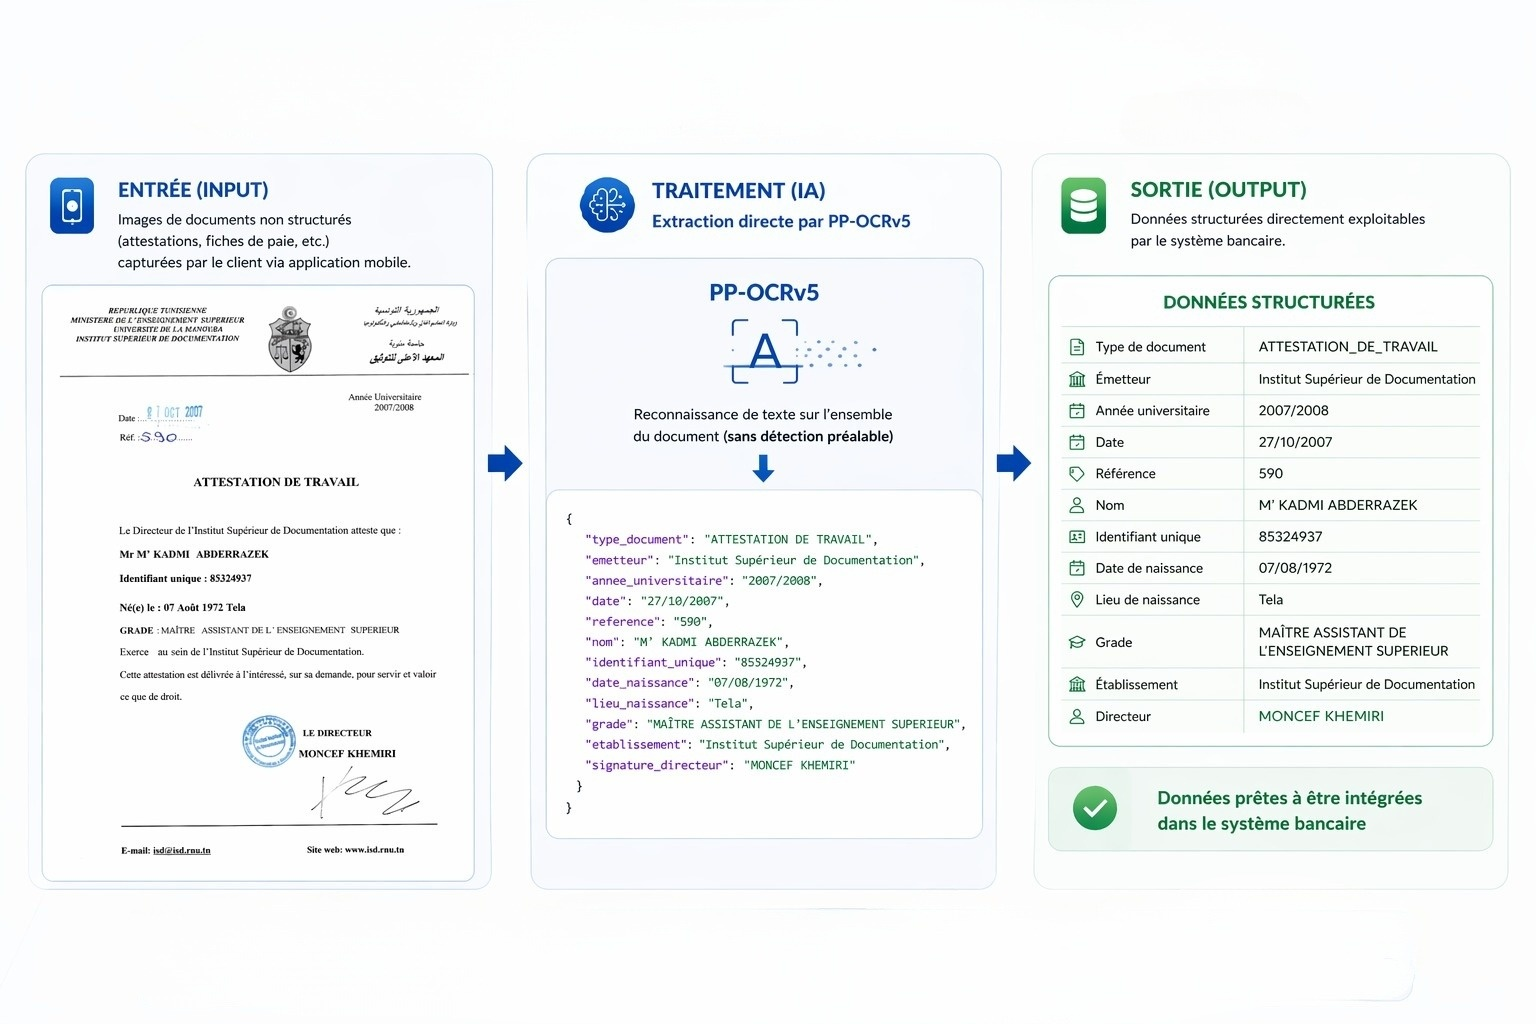
\includegraphics[width=0.75\textwidth]{images/image_ch3/pipline_1_phase.jpg}
  \caption{\textit{Pipeline CIN/Passeport}}
  \label{fig:ch3-pipeline-ia_cin-passeport}
\end{figure}

\textbf{Documents structurés (CIN, Passeport) :} une étape de détection d'objets (YOLO11m) précède l'extraction OCR. Cette approche en deux temps est nécessaire pour isoler avec précision les zones d'intérêt (données biométriques, numéro de série) sur des supports à géométrie variable.

\begin{figure}[H]
  \centering
  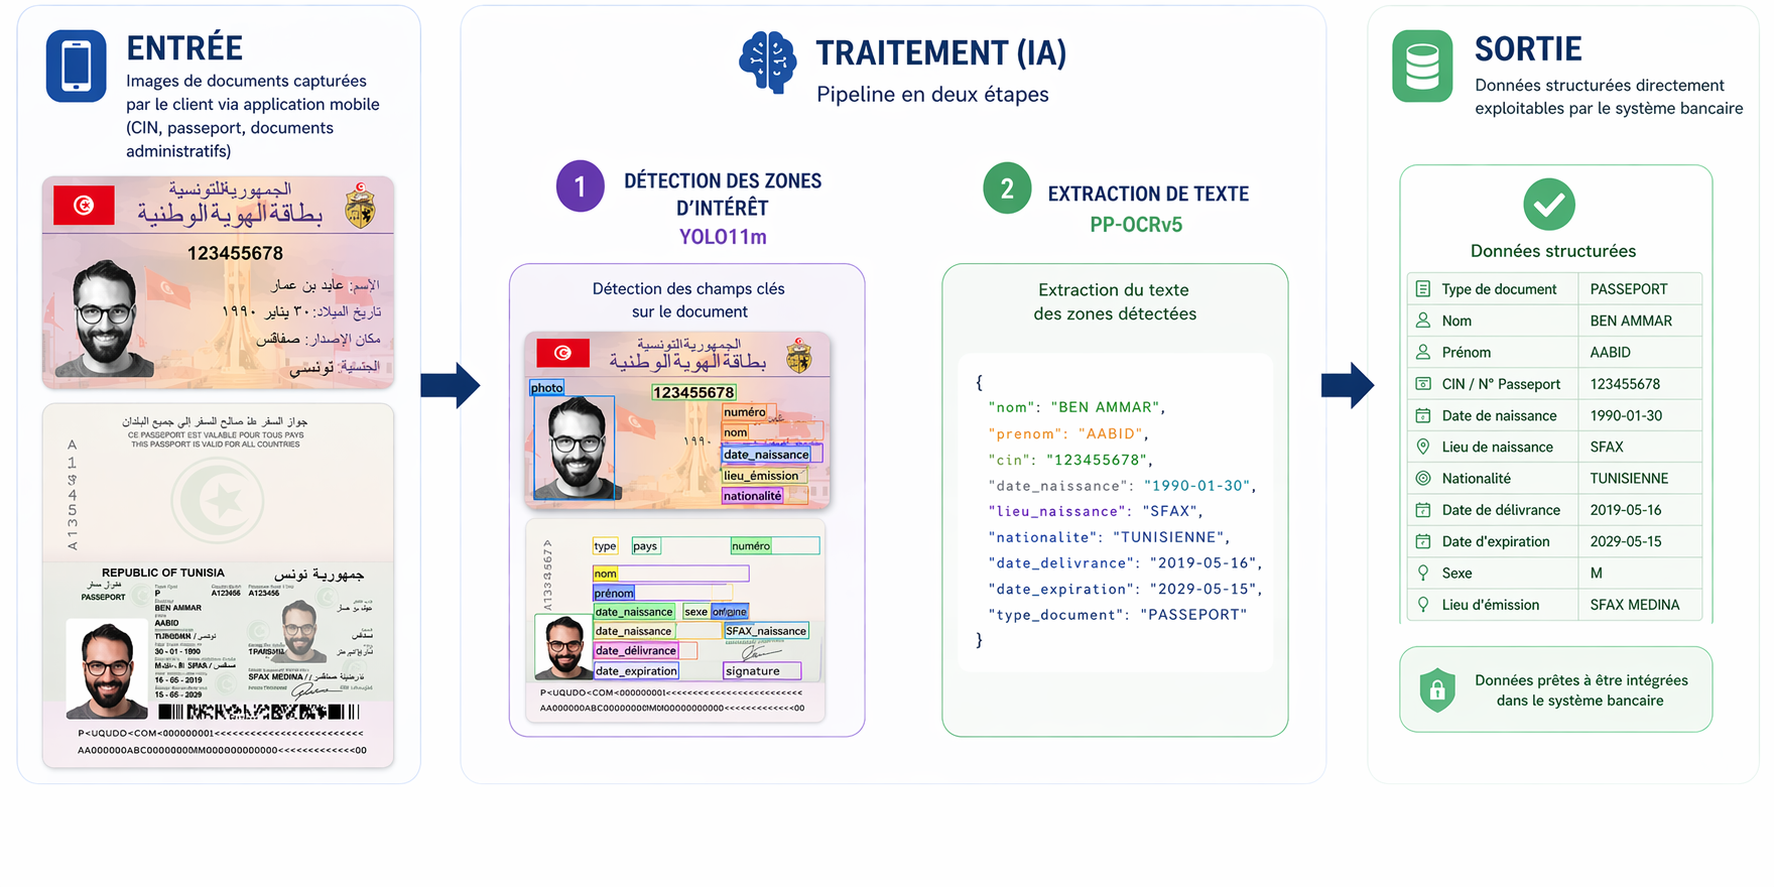
\includegraphics[width=0.75\textwidth]{images/image_ch3/pipline_2_phase.png}
  \caption{\textit{Pipeline autres documents}}
  \label{fig:ch3-pipeline-ia_autres-docs}
\end{figure}

\textbf{Documents non structurés (attestations, fiches de paie) :} l'extraction est réalisée directement par PP-OCRv5, sans étape de détection préalable. Cette rationalisation réduit sensiblement le temps d'inférence tout en maintenant une précision élevée sur des formats standardisés.

\subsection{Analyse des besoins documentaires}
\label{subsec:besoins-documentaires}

Chaque service bancaire implique un ensemble spécifique de documents à vérifier. Le tableau ci-dessous synthétise ces exigences et le pipeline IA correspondant.

\begin{table}[H]
  \centering
  \tiny
  \begin{tabular}{|l|l|l|}
    \toprule
    \rowcolor{bleu_principal}
    \textcolor{white}{\textbf{Service Métier}} & \textcolor{white}{\textbf{Documents Requis}} & \textcolor{white}{\textbf{Pipeline IA}} \\
    \midrule
    Ouverture de compte & CIN (recto/verso) ou Passeport & YOLO11m + PP-OCRv5 \\
    \midrule
    \rowcolor{gris_leger}
    Demande de crédit & CIN + Attestation de travail + Fiche de paie & YOLO11m + PP-OCRv5 (CIN) / PP-OCRv5 (docs fin.) \\
    \midrule
    Carte bancaire / Chéquier & Aucun document supplémentaire & Réutilisation données KYC \\
    \bottomrule
  \end{tabular}
  \caption{Matrice des documents requis par service et pipeline IA associé}
  \label{tab:ch3-besoins-doc}
\end{table}

Il convient de noter que le service carte bancaire et chéquier ne requiert aucune vérification documentaire supplémentaire : il s'appuie exclusivement sur le profil KYC déjà validé lors de l'ouverture de compte, ce qui allège le processus tout en garantissant la cohérence des données.

Cette cartographie des besoins documentaires oriente directement la stratégie de collecte et de constitution du dataset, présentée dans la section suivante.

\subsection{Collecte et composition du dataset}
\label{subsec:collecte-dataset}

La fiabilité d'une solution KYC bancaire ne repose pas sur la quantité brute de données, mais sur leur capacité à simuler l'imprévisibilité des conditions réelles : faible luminosité, arrière-plans complexes, captures mobiles en conditions non contrôlées. C'est sur ce principe qu'a été définie la stratégie de collecte.

\subsubsection*{Stratégie de collecte hybride}

Afin de construire un dataset à la fois structuré et robuste, deux canaux de collecte complémentaires ont été exploités :

\begin{itemize}
  \item \textbf{Open Source (Roboflow Universe) :} extraction de jeux de données préexistants comprenant des passeports internationaux et des échantillons de CIN tunisiennes, capturés en conditions idéales.

  \item \textbf{Données réelles (réseaux sociaux) :} collecte d'images de documents publiées en ligne (notamment des CIN déclarées perdues), présentant du bruit, des contre-jours et des masquages de confidentialité --- contraintes critiques reproduisant l'usage réel de l'application mobile.
\end{itemize}

\begin{table}[H]
  \centering
  \tiny
  \begin{tabular}{|l|p{3.5cm}|p{3.5cm}|p{3.5cm}|}
    \toprule
    \rowcolor{bleu_principal}
    \textcolor{white}{\textbf{Source}} & \textcolor{white}{\textbf{Avantage}} & \textcolor{white}{\textbf{Limite}} & \textcolor{white}{\textbf{Rôle}} \\
    \midrule
    Open Source (Roboflow) & Données propres, pré-annotées & Faible bruit --- peu réaliste & Pré-entraînement \\
    \midrule
    \rowcolor{gris_leger}
    Données réelles (réseaux sociaux) & Conditions réelles : bruit, contre-jour & Masquages agressifs & Robustesse \\
    \bottomrule
  \end{tabular}
  \caption{Analyse comparative des sources de données}
  \label{tab:ch3-sources-data}
\end{table}

La combinaison des deux sources compense leurs limites respectives --- l'open source apporte la structure, les données réelles apportent la robustesse face à l'imprévisibilité du terrain.

\subsubsection*{Distribution des classes}

Le dataset final totalise 685 instances, réparties de manière équilibrée entre les quatre classes d'intérêt :

\begin{table}[H]
  \centering
  \begin{tabular}{|l|c|c|l|}
    \toprule
    \rowcolor{bleu_principal}
    \textcolor{white}{\textbf{Classe}} & \textcolor{white}{\textbf{Instances}} & \textcolor{white}{\textbf{Proportion}} & \textcolor{white}{\textbf{Type de Traitement}} \\
    \midrule
    cinRecto & 200 & 29,2\% & YOLO11m + PP-OCRv5 \\
    \midrule
    \rowcolor{gris_leger}
    cinVerso & 202 & 29,5\% & YOLO11m + PP-OCRv5 \\
    \midrule
    passeport & 152 & 22,2\% & YOLO11m + PP-OCRv5 \\
    \midrule
    \rowcolor{gris_leger}
    Autre & 131 & 19,1\% & PP-OCRv5 (direct) \\
    \midrule
    \textbf{Total} & \textbf{685} & \textbf{100\%} & Hybride \\
    \bottomrule
  \end{tabular}
  \caption{Distribution du dataset par classe (source : Roboflow)}
  \label{tab:ch3-distribution-classes}
\end{table}

La quasi-parité entre cinRecto (200) et cinVerso (202) réflète une attention particulière à la couverture des deux faces de la CIN tunisienne, les deux étant requises lors de l'ouverture de compte. La classe Autre (131 instances) regroupe des captures partielles, des documents dégradés ou des images non identifiables --- utiles pour renforcer la robustesse du modèle face aux cas limites.

Si le sourcing réel apporte le réalisme nécessaire, il introduit un obstacle majeur : les données sont inexploitables en l'état à cause des masquages. Cela rend la phase suivante de Data Engineering (Restauration) non seulement utile, mais indispensable pour créer une vérité terrain supervisée.


%=============================================================
\section{Préparation des données (ingénierie des données)}
\label{sec:data-preparation}
%=============================================================

Les données collectées sur les réseaux sociaux, bien que cruciales pour le réalisme, posent un défi majeur de supervision : les masques de confidentialité --- traits de feutre, bandes noires, flous numériques --- empêchent YOLO d'apprendre la structure complète et les points d'ancrage réels des documents. Pour transformer ces données inexploitables en une vérité terrain (Ground Truth) de haute précision, deux stratégies complémentaires ont été déployées, adaptées à la complexité de chaque face du document.

\subsection{Restauration et génération de données}
\label{subsec:restauration-generation}

\subsubsection*{CIN recto --- restauration par Deep Inpainting}

Pour le recto, l'enjeu était double : conserver l'authenticité visuelle de la photo d'identité et du fond, tout en rendant le numéro de carte exploitable par l'OCR. Le processus se déroule en trois phases :

\begin{itemize}
  \item \textbf{Nettoyage localisé :} application d'algorithmes de Deep Inpainting (via ObjectRemover) sur la zone du numéro masqué. L'IA reconstruit les motifs de sécurité (guillochis) en analysant les pixels environnants.

  \item \textbf{Réinjection typographique :} superposition d'un numéro de remplacement dans la police OCR-B (norme ISO) via Figma, garantissant alignement et espacement identiques aux documents officiels.

  \item \textbf{Réalisme contextuel :} chaque insertion respecte la signature optique d'origine par Blur Matching (flou gaussien calibré sur le grain du capteur) et Glare Integration (fusion avec les zones de surexposition), éliminant toute « anomalie de perfection » qui trahirait l'origine synthétique de la donnée.
\end{itemize}

\begin{figure}[H]
  \centering
  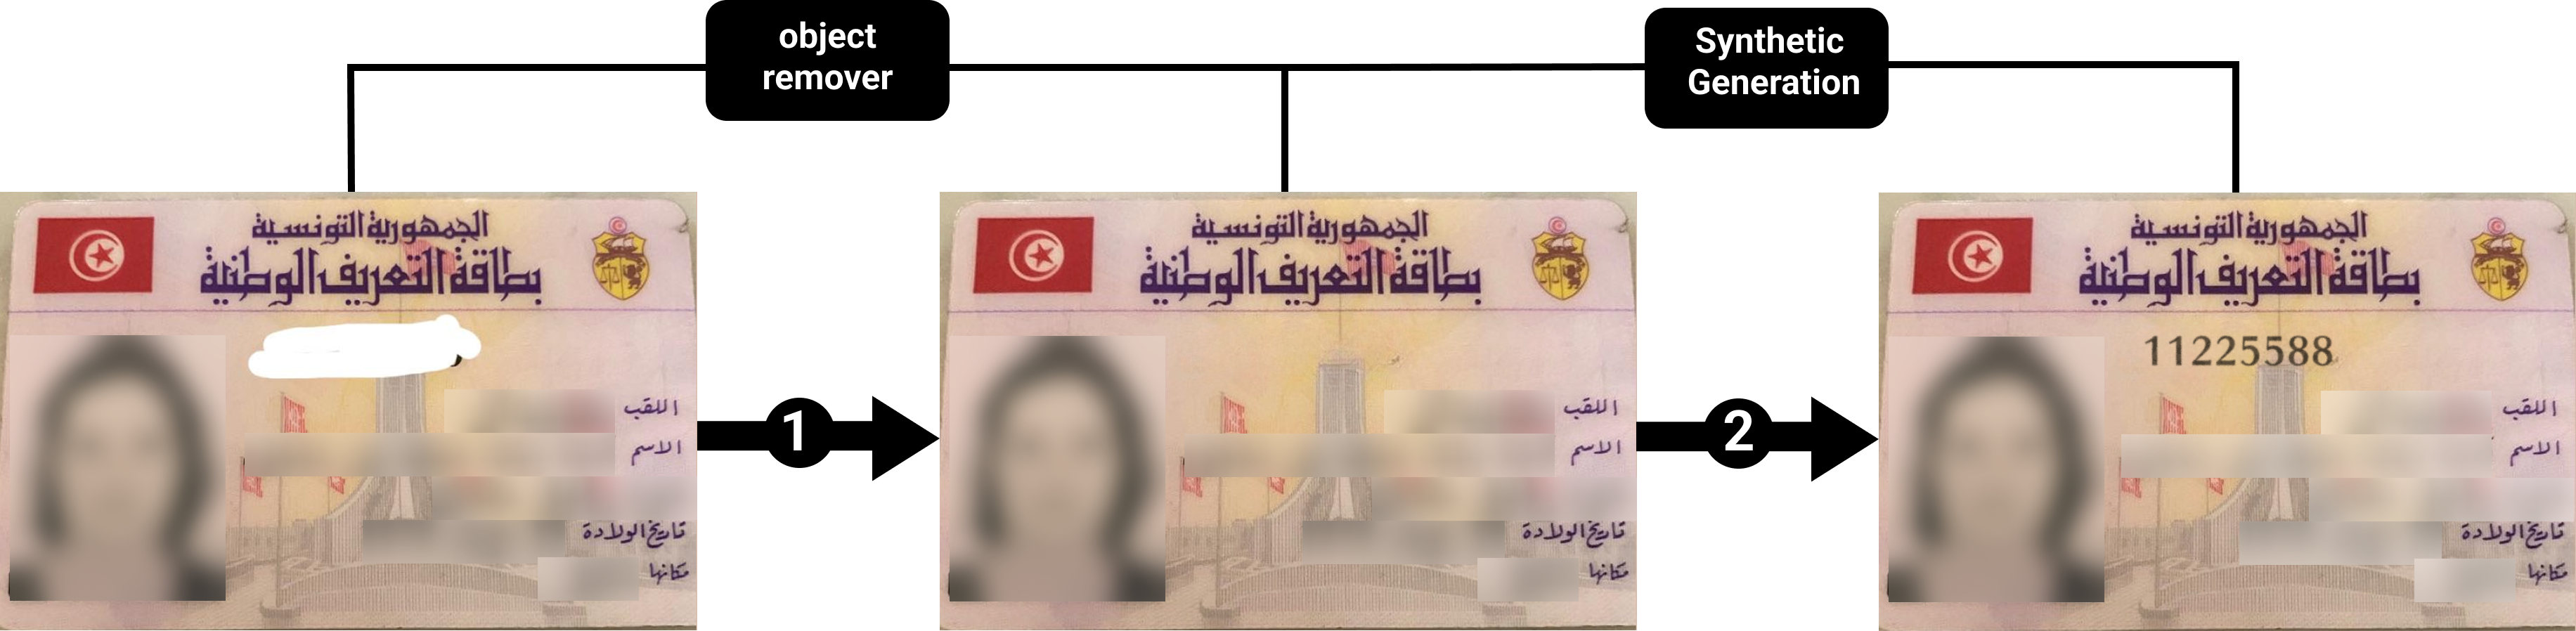
\includegraphics[width=0.75\textwidth]{images/image_ch3/Processus de_restauration_CIN Recto.png}
  \caption{\textit{Figure 3.1 --- Processus de restauration CIN Recto}}
  \label{fig:ch3-restauration-recto}
\end{figure}

\begin{figure}[H]
  \centering
  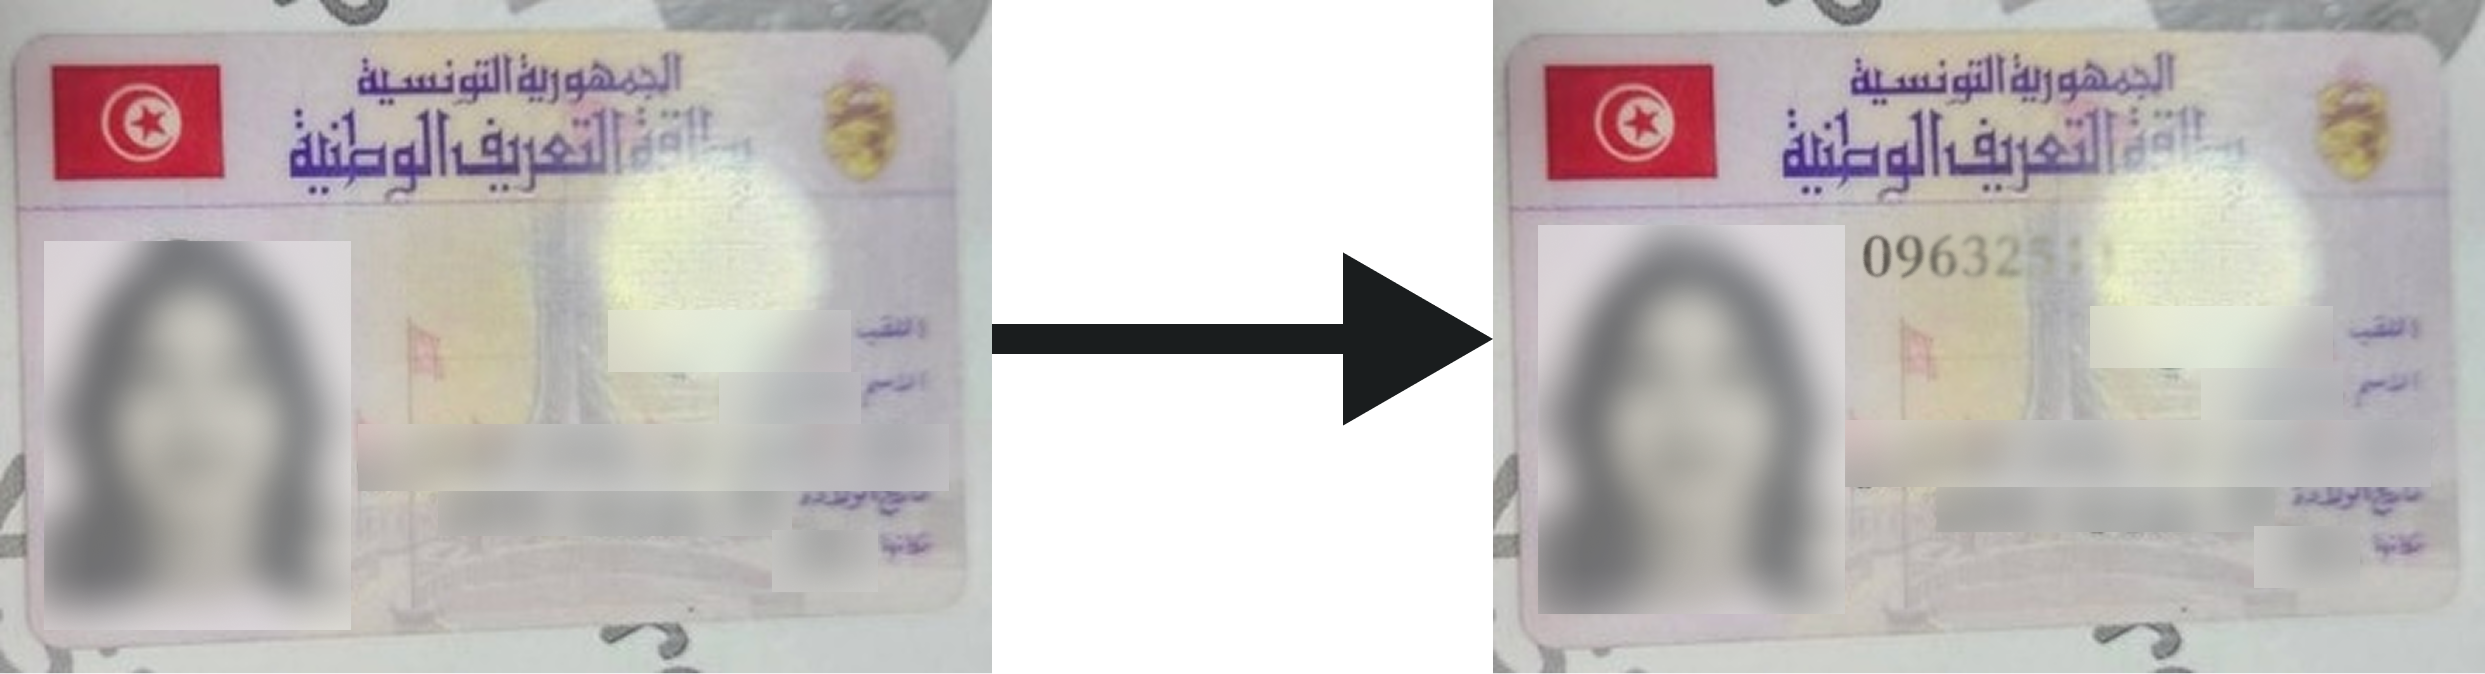
\includegraphics[width=0.75\textwidth]{images/image_ch3/Simulation_de_contraintes_optiques réelles.png}
  \caption{\textit{Figure 3.2 --- Simulation de contraintes optiques réelles}}
  \label{fig:ch3-contraintes-optiques}
\end{figure}

\subsubsection*{CIN verso --- génération automatisée par Data Factory Python}

Le verso, dont la densité textuelle est plus élevée, nécessitait une approche différente. Plutôt que de traiter chaque image individuellement, nous avons créé une matrice de génération à partir d'un document authentique :

\begin{itemize}
  \item \textbf{Génération du template de base :} plutôt que de dessiner un fond artificiel, nous avons pris une image de CIN réelle dont nous avons intégralement effacé les mentions textuelles via ObjectRemover. Le résultat est un template nu qui conserve la texture physique authentique --- grain numérique, ombres portées, irrégularités d'éclairage --- d'un document téléversé par mobile.

  \item \textbf{Data Factory Python :} un script automatise le remplissage des champs (Nom, Prénom du père, Mère, Adresse) en générant des identités aléatoires positionnées avec précision sur le template. Cette méthode produit des centaines de variantes parfaitement étiquetées sur un support qui « trompe » l'œil du modèle en lui faisant croire qu'il traite un document 100\% réel.
\end{itemize}

\begin{figure}[H]
  \centering
  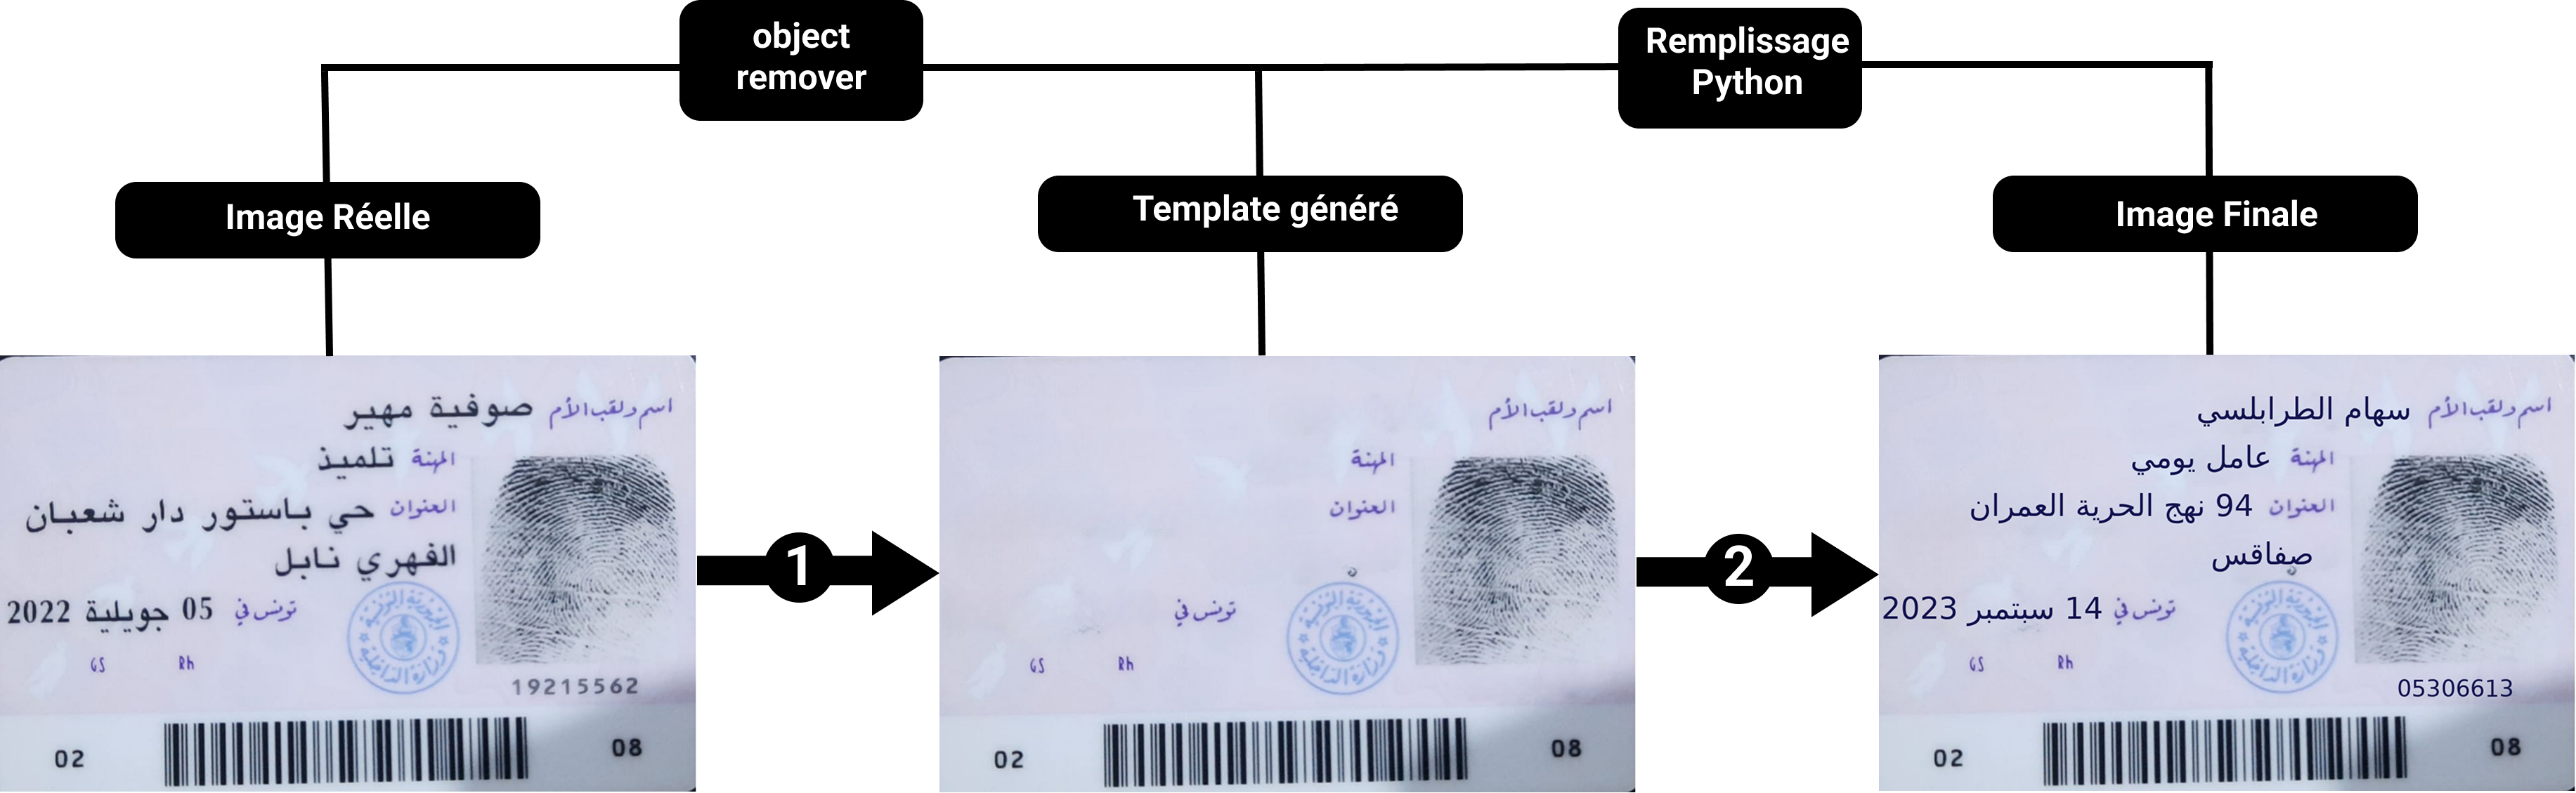
\includegraphics[width=0.75\textwidth]{images/image_ch3/Pipeline_creation_template_verso.png}
  \caption{\textit{Figure 3.3 --- Pipeline de création du template Verso}}
  \label{fig:ch3-template-verso}
\end{figure}

Une fois ce dataset restauré et enrichi, il convient de lui donner un sens mathématique pour l'IA. La phase de labellisation intervient alors pour définir précisément les zones d'intérêt, transformant les images brutes en données d'apprentissage supervisé.

\subsection{Labellisation : construction de la vérité terrain}
\label{subsec:labellisation}

Une fois le dataset restauré, il convient de lui donner un sens mathématique pour l'IA. La labellisation consiste à définir des Bounding Boxes autour de chaque champ critique, transformant les images brutes en données d'apprentissage supervisé.

\subsubsection*{Ontologie des classes}

Trois ontologies distinctes ont été définies selon le type de document :

\begin{itemize}
  \item \textbf{CIN Recto :} address, cin, dob, first\_name, flag1, flag2, full\_name, header\_text, image, last\_name, num\_cin, pob.

  \item \textbf{CIN Verso :} address, barcode, finger\_print, flag3, issue\_date, mother\_name, print\_id, profession.

  \item \textbf{Passeport :} address, dob, first\_name, image, last\_name, num\_cin, pob, num\_pass.
\end{itemize}

\subsubsection*{Méthodologie hybride : du Gold Standard à l'Auto-Labeling}

Face au volume de données à annoter, une approche hybride en trois phases a été adoptée pour concilier efficacité et précision :

\begin{enumerate}
  \item \textbf{Amorçage manuel (Gold Standard) :} labellisation manuelle des 50 premières images de chaque catégorie sur Roboflow, constituant un jeu de référence de haute précision.

  \item \textbf{Auto-labeling assisté :} un modèle YOLO pré-entraîné sur ces 50 images suggère automatiquement les boîtes sur les images restantes, réduisant considérablement le temps d'annotation.

  \item \textbf{Vérification humaine systématique :} chaque boîte suggérée est ajustée manuellement pour que ses bords touchent exactement les caractères --- condition critique pour la qualité de l'extraction OCR.
\end{enumerate}

\subsubsection*{Contrainte des Tight Bounding Boxes}

Une règle stricte a été appliquée : la boîte doit englober le texte au pixel près sans inclure de bruit environnant. Une boîte trop large incorpore des éléments décoratifs qui perturbent l'OCR ; une boîte trop serrée coupe les jambages de certains caractères (tels que 'p' ou 'q'), dégradant la précision de la reconnaissance. Cette rigueur constitue la condition sine qua non d'une extraction OCR performante.

\begin{figure}[H]
  \centering
  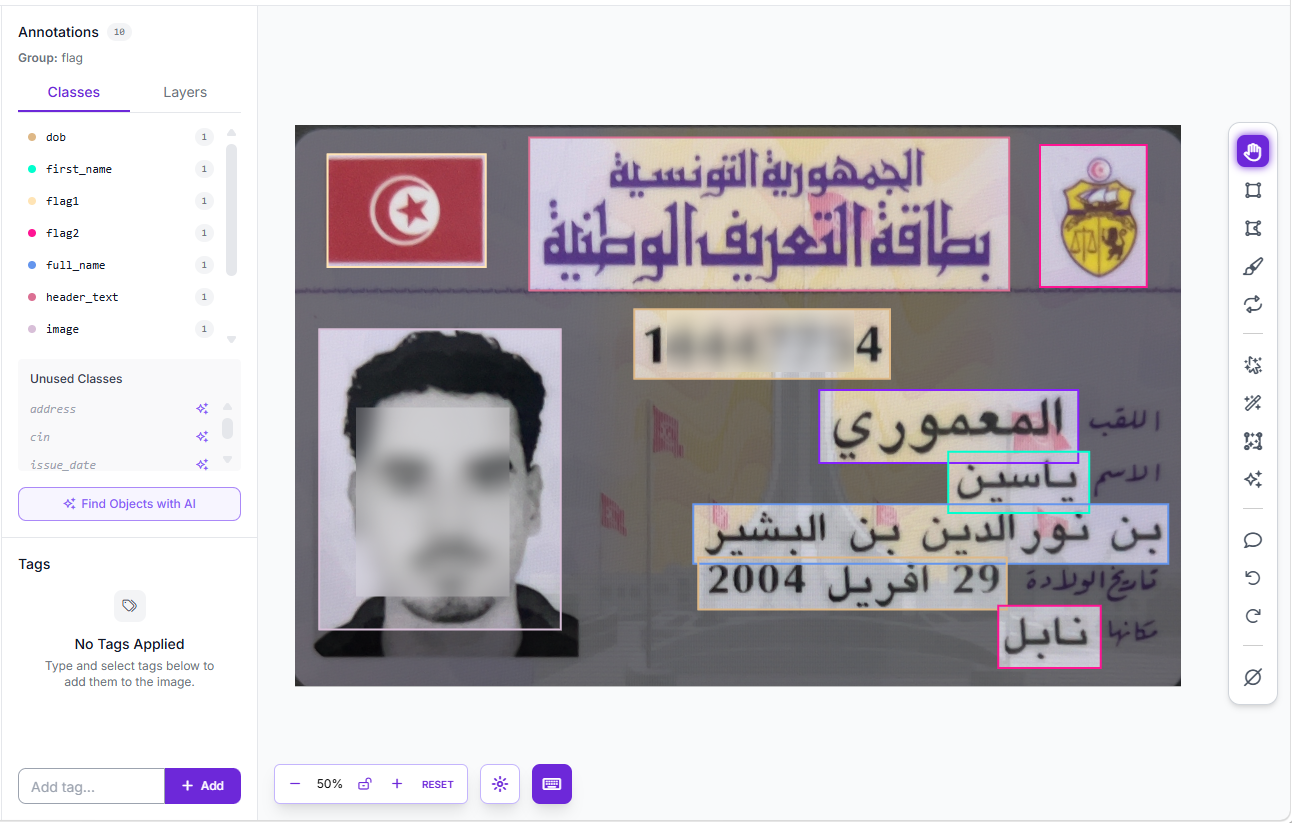
\includegraphics[width=0.75\textwidth]{images/image_ch3/roboflow.png}
  \caption{\textit{Interface Roboflow illustrant la précision des Tight Bounding Boxes sur une CIN}}
  \label{fig:ch3-bounding-boxes}
\end{figure}

Le dataset ainsi labellisé constitue une base d'apprentissage rigoureuse. Cependant, 685 instances restent insuffisantes pour garantir la robustesse du modèle face aux aléas d'une capture mobile réelle. La phase d'augmentation contrôlée répond à ce défi.

\subsection{Augmentation contrôlée : simulation de la variabilité réelle}
\label{subsec:augmentation}

Plutôt qu'une augmentation aléatoire, nous avons appliqué une stratégie différenciée selon la complexité de chaque tâche pour éviter le surapprentissage via la plateforme Roboflow, simulant les contraintes physiques du monde réel tout en évitant le surapprentissage.

\subsubsection*{Coefficients d'augmentation différenciés}

Le volume final a été calibré pour éviter le surapprentissage tout en assurant une couverture représentative des scénarios réels :

\begin{table}[H]
  \centering
  \begin{tabular}{|l|c|c|c|l|}
    \toprule
    \rowcolor{bleu_principal}
    \textcolor{white}{\textbf{Pipeline}} & \textcolor{white}{\textbf{Source}} & \textcolor{white}{\textbf{Coefficient}} & \textcolor{white}{\textbf{Total}} & \textcolor{white}{\textbf{Focus}} \\
    \midrule
    Classification Globale & 473 & ×10 & 4\,730 & Invariance contextuelle globale \\
    \midrule
    \rowcolor{gris_leger}
    CIN Recto & 712 & ×4 & 2\,884 & Perspective et alignement YOLO \\
    \midrule
    CIN Verso & 182 & ×4 & 728 & Précision OCR et netteté \\
    \midrule
    \rowcolor{gris_leger}
    Passeport & 158 & ×4 & 644 & Précision OCR et netteté \\
    \bottomrule
  \end{tabular}
  \caption{Coefficients d'augmentation par pipeline et volumes finaux obtenus}
  \label{tab:ch3-augmentation-coeff}
\end{table}

\subsubsection*{Paramètres d'augmentation et impacts visuels}

Trois axes de transformation ont été retenus, chacun répondant à une contrainte physique identifiée :

\paragraph{A. Invariance spatiale (géométrie \& perspective)}

Ces transformations compensent les erreurs de manipulation humaine. Un utilisateur ne tient jamais son smartphone parfaitement parallèle au document, ce qui crée des distorsions géométriques.

\begin{figure}[H]
  \centering
  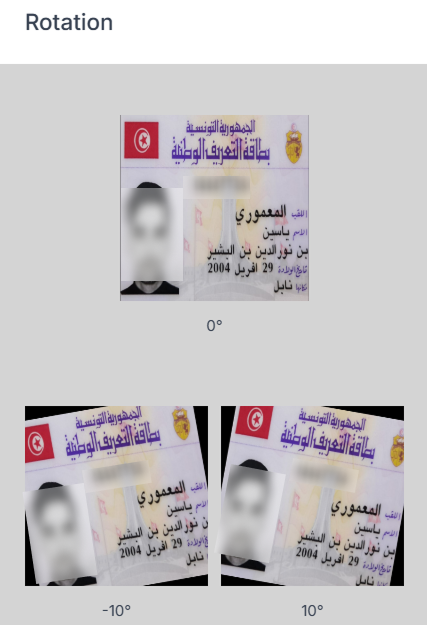
\includegraphics[width=0.75\textwidth]{images/image_ch3/rotation.png}
  \caption{\textit{Illustration de l'augmentation par rotation ($-$10°, 0°, +10°)}}
  \label{fig:ch3-rotation}
\end{figure}

\begin{itemize}
  \item \textbf{Rotation :} indispensable pour que YOLO détecte la carte même si elle est présentée de travers.
\end{itemize}

\paragraph{B. Invariance photométrique (lumière \& couleur)}

L'objectif est de rendre l'extraction d'information indépendante de l'éclairage ambiant ou de la qualité du capteur.

\begin{figure}[H]
  \centering
  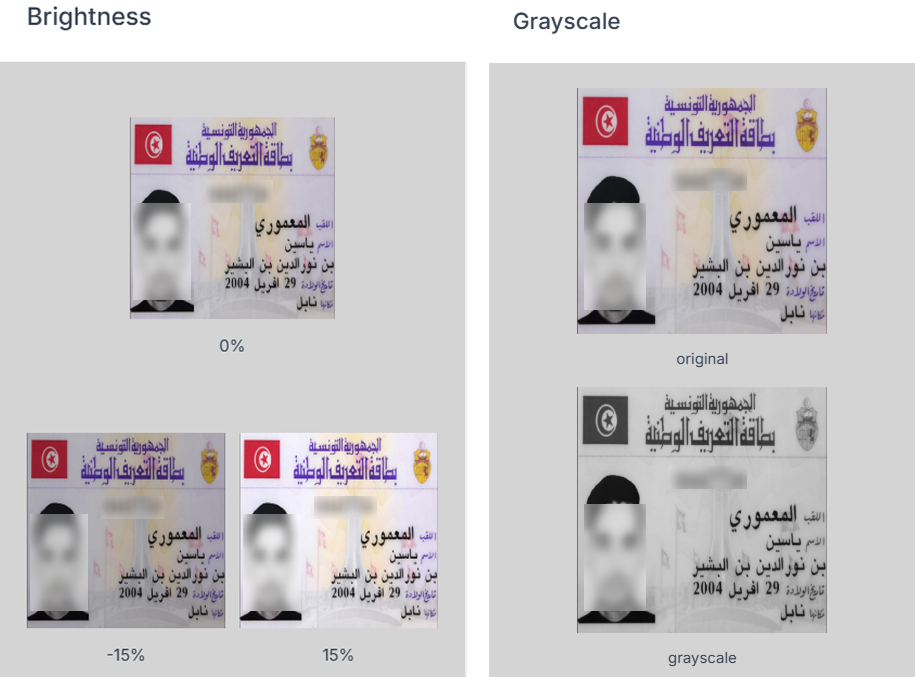
\includegraphics[width=0.75\textwidth]{images/image_ch3/lumino_grayscale.png}
  \caption{\textit{Illustration de l'augmentation photométrique : variations de luminosité et niveaux de gris}}
  \label{fig:ch3-photometrie}
\end{figure}

\begin{itemize}
  \item \textbf{Luminosité :} reproduit les variations entre une pièce sombre et un éclairage direct (éblouissement par le flash).

  \item \textbf{Grayscale :} habitue le modèle à reconnaître la structure de la CIN même sur des captures en noir et blanc ou des photocopies de faible qualité.
\end{itemize}

\paragraph{C. Résilience optique (flou \& bruit capteur)}

\begin{figure}[H]
  \centering
  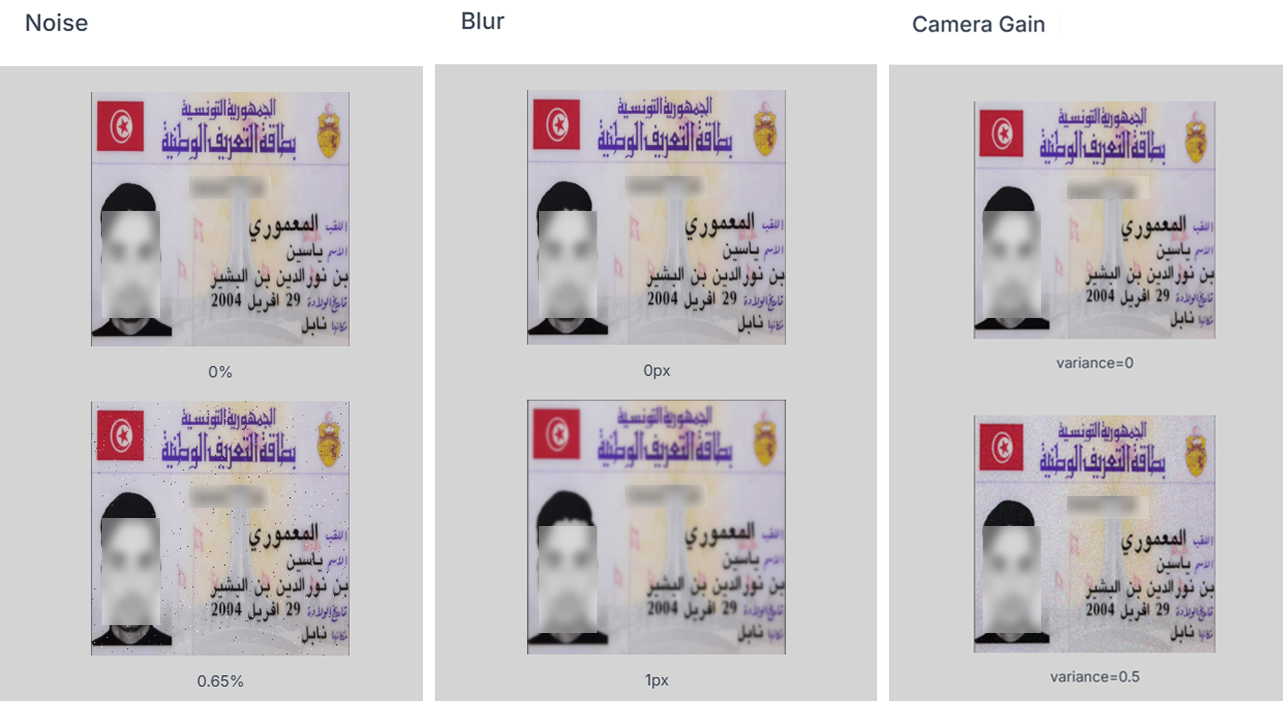
\includegraphics[width=0.75\textwidth]{images/image_ch3/bruit_flou_gainCamera.png}
  \caption{\textit{Illustration de la résilience optique : bruit, flou et gain de caméra}}
  \label{fig:ch3-resilience-optique}
\end{figure}

\begin{itemize}
  \item \textbf{Bruit :} ajout de grain pour simuler les capteurs de smartphones d'entrée de gamme en basse lumière.

  \item \textbf{Gain de caméra :} simule l'amplification ISO pour la robustesse à l'exposition.

  \item \textbf{Flou :} modélise les imprécisions de mise au point pour forcer l'extraction de traits robustes.
\end{itemize}

\subsubsection*{Configurations Roboflow par pipeline}

\begin{table}[H]
  \centering
  \small
  \begin{tabular}{|l|c|c|c|c|}
    \toprule
    \rowcolor{bleu_principal}
    \textcolor{white}{\textbf{Paramètre}} & \textcolor{white}{\textbf{Classification}} & \textcolor{white}{\textbf{CIN Recto}} & \textcolor{white}{\textbf{CIN Verso}} & \textcolor{white}{\textbf{Passeport}} \\
    \midrule
    Sorties / exemple & 3 & 4 & 4 & 4 \\
    \midrule
    \rowcolor{gris_leger}
    Rotation & ±10° & ±10° & ±10° & ±5° \\
    \midrule
    Niveaux de gris & --- & 5\% images & 5\% images & --- \\
    \midrule
    \rowcolor{gris_leger}
    Luminosité & ±25\% & ±10\% & ±10\% & ±15\% \\
    \midrule
    Flou simple & $\leq$1 px & $\leq$0,5 px & $\leq$0,5 px & $\leq$0,4 px \\
    \midrule
    \rowcolor{gris_leger}
    Bruit & $\leq$0,69\% & $\leq$0,3\% & $\leq$0,3\% & $\leq$0,3\% \\
    \midrule
    Gain de caméra & --- & 0,06\% & 0,06\% & --- \\
    \midrule
    \rowcolor{gris_leger}
    \textbf{Total dataset} & \textbf{4\,932} & \textbf{3\,004} & \textbf{806} & \textbf{709} \\
    \bottomrule
  \end{tabular}
  \caption{Configurations Roboflow par pipeline}
  \label{tab:ch3-roboflow-config}
\end{table}

Cette stratégie d'augmentation a pour objectif d'enrichir notre base d'entraînement avec un volume de données diversifié, permettant ainsi au modèle d'affiner ses capacités d'apprentissage et d'améliorer sa précision globale.

Le dataset ainsi constitué --- restauré, labellisé et augmenté --- offre une base d'entraînement solide. La section suivante détaille l'architecture du pipeline IA retenu et les paramètres d'entraînement associés.


%=============================================================
\section{Modélisation}
\label{sec:modelisation}
%=============================================================

Le dataset ainsi constitué --- restauré, labellisé et augmenté --- constitue le socle sur lequel reposent les décisions de modélisation. Cette section décrit l'architecture du pipeline IA retenu et les paramètres d'entraînement pour chacun des modèles développés.

%-------------------------------------------------------------
\subsection{Architecture globale du système IA}
\label{subsec:architecture-ia}
%-------------------------------------------------------------

Le système IA est structuré en deux pipelines distincts selon la nature du document traité (voir Figure~\ref{fig:ch3-pipeline-ia_cin-passeport} et Figure~\ref{fig:ch3-pipeline-ia_autres-docs}, section 3.1.1). Pour les documents structurés --- CIN et passeport --- le pipeline enchaîne quatre services indépendants exposés chacun via une API REST FastAPI :

\begin{enumerate}
  \item \textbf{Service de classification} (port 8005) : reçoit l'image capturée et identifie le type de document parmi cinq classes (\texttt{CIN\_RECTO}, \texttt{CIN\_VERSO}, \texttt{PASSPORT}, \texttt{ATTESTATION\_TRAVAIL}, \texttt{FICHE\_PAIE}) grâce à un modèle YOLOcls.
  \item \textbf{Service de capture} (ports 8001/8006) : détecte la présence du document dans le flux vidéo en temps réel via YOLOv8n et déclenche la capture automatique dès stabilisation.
  \item \textbf{Service OCR} (port 8002) : localise les champs par YOLOv11m, recadre chaque zone et en extrait le texte via PaddleOCR PP-OCRv5.
  \item \textbf{Service de comparaison faciale} (port 8007) : capture le selfie et compare la photo extraite du document avec le visage de l'utilisateur.
\end{enumerate}

Ce découplage en microservices garantit qu'une mise à jour d'un modèle n'impacte aucun autre service, conformément aux exigences de maintenabilité définies en section 4.3.

%-------------------------------------------------------------
\subsection{Détection de présence du document --- YOLOv8n}
\label{subsec:yolov8n-presence}
%-------------------------------------------------------------

Avant toute extraction, le système doit s'assurer que le document est correctement cadré et de qualité suffisante. Ce rôle est assuré par trois services de capture exploitant chacun un modèle YOLOv8n léger, adapté à une inférence en temps réel sur flux vidéo :

\begin{itemize}
  \item \texttt{capture-cin} (port 8001) : CIN recto et verso.
  \item \texttt{capture-passport} (port 8006) : passeport.
  \item \texttt{capture-face} (port 8007) : selfie biométrique.
\end{itemize}

\noindent\textbf{Paramètres de détection.} Chaque frame est analysée à 640 $\times$ 640 pixels avec :

\begin{itemize}
  \item Seuil de détection : 0,25 (sensibilité maximale).
  \item Seuil de validation métier : 0,50 (décision de capture).
  \item Stabilisation : 5 frames consécutives valides requises avant déclenchement, éliminant les fausses confirmations dues aux mouvements brusques.
  \item Stockage : image recadrée et agrandie, enregistrée dans MinIO à 97\,\% de qualité JPEG pour préserver la lisibilité OCR en aval.
\end{itemize}

\noindent\textbf{États retournés au frontend.} Le service communique trois états en temps réel guidant l'utilisateur sans action manuelle :

\begin{itemize}
  \item \texttt{ABSENT} : aucun document détecté dans le cadre.
  \item \texttt{DETECTED} : document présent mais pas encore stabilisé.
  \item \texttt{CONFIRMED} : capture validée, transmission au pipeline OCR.
\end{itemize}

Ce service constitue le verrou qualité d'entrée du pipeline.

%-------------------------------------------------------------
\subsection{Détection des champs texte --- YOLOv11m}
\label{subsec:yolov11m-champs}
%-------------------------------------------------------------

Comme établi au chapitre 2, YOLOv11m a été retenu pour sa supériorité en précision de localisation sur des objets de petite taille dans des images à haute résolution. Il intervient ici non pour détecter des objets génériques, mais pour localiser avec précision chaque champ textuel sur un document d'identité.

\subsubsection*{Stratégie : trois modèles spécialisés}

La décision de former trois modèles distincts --- un par type de document --- répond à une contrainte fondamentale : les ontologies de classes sont incompatibles entre documents.

\begin{itemize}
  \item \textbf{CIN Recto} : 12 classes incluant \texttt{last\_name}, \texttt{first\_name}, \texttt{full\_name}, \texttt{num\_cin}, \texttt{dob}, \texttt{pob}, \texttt{image}, \texttt{header\_text}, \texttt{flag1}, \texttt{flag2}. La disposition est arabe de droite à gauche, avec des zones de texte compactes.
  \item \textbf{CIN Verso} : 8 classes dont \texttt{mother\_name}, \texttt{profession}, \texttt{address}, \texttt{issue\_date}, \texttt{print\_id}, \texttt{barcode}, \texttt{finger\_print}, \texttt{flag3}. Le champ adresse est multi-lignes et occupe une surface importante.
  \item \textbf{Passeport} : champs bilingues arabe/latin, \texttt{last\_name}, \texttt{first\_name}, \texttt{num\_pass}, \texttt{num\_cin}, \texttt{dob}, \texttt{pob}, \texttt{image}, \texttt{address}. Format portrait ($3$:$4$), densité textuelle plus forte.
\end{itemize}

Un modèle unique entraîné sur les trois documents produirait des ambiguïtés de classes (un champ \texttt{dob} sur la CIN et un champ \texttt{dob} sur le passeport n'ont pas le même format ni la même position) et dégraderait la précision des bounding boxes.

\subsubsection*{Paramètres d'entraînement}

Les trois modèles partagent la même architecture de base YOLOv11m pré-entraînée sur COCO, avec un \textit{fine-tuning} par transfert d'apprentissage. Le Tableau~\ref{tab:ch3-params-yolo} présente les paramètres comparatifs.

\small
\begin{longtable}{|l|c|c|c|}
  \rowcolor{bleu_principal}
  \textcolor{white}{\textbf{Paramètre}} & \textcolor{white}{\textbf{CIN Recto}} & \textcolor{white}{\textbf{CIN Verso}} & \textcolor{white}{\textbf{Passeport}} \\
  \endfirsthead
  \rowcolor{bleu_principal}
  \textcolor{white}{\textbf{Paramètre}} & \textcolor{white}{\textbf{CIN Recto}} & \textcolor{white}{\textbf{CIN Verso}} & \textcolor{white}{\textbf{Passeport}} \\
  \endhead
  \midrule
  Images originales & 712 & 532 & 488 \\
  \midrule
  \rowcolor{gris_leger}
  Coefficient augmentation & $\times$4 & $\times$4 & $\times$3 \\
  \midrule
  Images entraînement & 2\,848 & 2\,128 & 1\,464 \\
  \midrule
  \rowcolor{gris_leger}
  Images validation & 156 & 148 & 137 \\
  \midrule
  Images test & 70 & 60 & 50 \\
  \midrule
  \rowcolor{gris_leger}
  Résolution & 1280 $\times$ 1280 px & 1280 $\times$ 1280 px & 1280 $\times$ 1280 px \\
  \midrule
  Batch size & 8 & 8 & 8 \\
  \midrule
  \rowcolor{gris_leger}
  Époques max & 150 & 150 & 150 \\
  \midrule
  Patience (early stop) & 40 & 40 & 40 \\
  \midrule
  \rowcolor{gris_leger}
  Optimiseur & AdamW & AdamW & AdamW \\
  \midrule
  Taux d'apprentissage $lr_0$ & 0,001 & 0,001 & 0,001 \\
  \midrule
  \rowcolor{gris_leger}
  $lr$ final ($lrf$) & 0,01 & 0,01 & 0,01 \\
  \midrule
  Weight decay & 0,0003 & 0,0003 & 0,0004 \\
  \midrule
  \rowcolor{gris_leger}
  Warmup époques & 3 & 3 & 3 \\
  \midrule
  Scheduler LR & Cosinus & Cosinus & Cosinus \\
  \midrule
  \rowcolor{gris_leger}
  Loss box & 7,5 & 7,5 & 7,5 \\
  \midrule
  Loss cls & 0,5 & 0,5 & 0,4 \\
  \midrule
  \rowcolor{gris_leger}
  Loss dfl & 1,5 & 1,5 & 1,5 \\
  \midrule
  Scale (augmentation) & 0,20 & 0,10 & 0,15 \\
  \midrule
  \rowcolor{gris_leger}
  Translate & 0,03 & 0,04 & 0,04 \\
  \midrule
  Degrees & 2,0° & 2,0° & 3,0° \\
  \midrule
  \rowcolor{gris_leger}
  Mosaic / Mixup / Flip & Désactivés & Désactivés & Désactivés \\
  \bottomrule
  \caption{Paramètres comparatifs d'entraînement des trois modèles YOLOv11m}
  \label{tab:ch3-params-yolo}
\end{longtable}
\normalsize

Plusieurs choix méritent d'être explicités :

\begin{itemize}
  \item \textbf{Résolution 1\,280 $\times$ 1\,280 px :} les champs texte comme \texttt{num\_cin} ou \texttt{dob} occupent moins de 80 pixels de hauteur sur un document photographié de face --- une résolution de 640 px les rendrait illisibles pour l'OCR en aval.
  \item \textbf{Weight decay passeport (0,0004) :} légèrement supérieur à celui de la CIN (0,0003) pour compenser un dataset plus réduit (1\,464 images contre 2\,848).
  \item \textbf{Scale verso réduit à 0,10 :} protège la zone MRZ (\textit{Machine Readable Zone}) en bas de carte, dont une déformation excessive casserait la structure de lecture.
  \item \textbf{Mosaic / Mixup / Flip désactivés :} un document retourné ou composite n'existe pas en production --- ces augmentations introduiraient des cas irréalistes.
\end{itemize}

\subsubsection*{Résultats d'entraînement}

% ── Bloc YOLO ────────────────────────────────────────────────
\begin{tcolorbox}[
  enhanced,
  breakable,
  colback    = yolo_bg,
  colframe   = yolo_border,
  arc        = 4pt,
  boxrule    = 1.2pt,
  drop shadow,
  attach boxed title to top left = {yshift=-3mm, xshift=8mm},
  boxed title style = {
    colback   = yolo_header,
    colframe  = yolo_border,
    arc       = 3pt,
    boxrule   = 0.8pt,
    fontupper = \bfseries\color{white}\small
  },
  title = {\faSearch\quad Métriques de détection d'objets --- YOLO}
]

\noindent Les performances du modèle YOLOv11m sont évaluées selon les métriques standard d'Ultralytics, adaptées ici à la détection de champs textuels sur documents d'identité.

\medskip
\noindent\textbf{Concepts fondamentaux.} Toute prédiction est classée en l'une des quatre catégories :

\smallskip
\begin{center}
\small
\begin{tabular}{>{\bfseries}l p{9cm}}
  \rowcolor{bleu_principal!12}
  Catégorie & Signification dans le contexte KYC \\[2pt]
  \midrule
  TP & Le modèle détecte un champ textuel qui existe réellement sur le document. \\[3pt]
  FP & Le modèle prédit un champ absent du document (fausse alarme). \\[3pt]
  FN & Le modèle rate un champ présent --- champ critique manqué. \\[3pt]
  TN & Aucune détection là où aucun champ n'est attendu. \\
\end{tabular}
\end{center}

\medskip
\noindent\textbf{Métriques dérivées.}

\medskip

% Précision
\noindent\textcolor{bleu_clair}{\ding{72}}\; \textcolor{bleu_clair}{\textbf{Précision (Precision) :}}

\noindent La précision mesure la fiabilité des détections : sur toutes les zones prédites comme champs, combien sont effectivement des champs réels ?

\begin{equation*}
  P = \frac{TP}{TP + FP}
\end{equation*}

\noindent où $TP$ est le nombre de vrais positifs et $FP$ le nombre de faux positifs. Une précision élevée signifie peu de faux cadres autour de zones sans texte.

\medskip

% Rappel
\noindent\textcolor{bleu_clair}{\ding{72}}\; \textcolor{bleu_clair}{\textbf{Rappel (Recall) :}}

\noindent Le rappel mesure le taux de couverture : sur tous les champs présents dans le document, combien le modèle en a-t-il détectés ?

\begin{equation*}
  R = \frac{TP}{TP + FN}
\end{equation*}

\noindent où $FN$ est le nombre de faux négatifs. Un rappel élevé garantit qu'aucun champ critique (\texttt{num\_cin}, \texttt{dob}) n'est omis.

\medskip

% F1
\noindent\textcolor{bleu_clair}{\ding{72}}\; \textcolor{bleu_clair}{\textbf{Score F1 :}}

\noindent Moyenne harmonique de la précision et du rappel, synthétisant les deux en un seul indicateur équilibré.

\begin{equation*}
  F_1 = \frac{2 \times P \times R}{P + R}
\end{equation*}

\medskip

% IoU
\noindent\textcolor{bleu_clair}{\ding{72}}\; \textcolor{bleu_clair}{\textbf{IoU (\textit{Intersection over Union}) :}}

\noindent Mesure la précision spatiale de la boîte prédite en calculant le chevauchement entre la boîte prédite $\hat{B}$ et la vérité terrain $B$.

\begin{equation*}
  \text{IoU} = \frac{\text{Aire}(\hat{B} \cap B)}{\text{Aire}(\hat{B} \cup B)}
\end{equation*}

\noindent Un score de 1 indique une superposition parfaite — condition indispensable pour que le crop transmis à PaddleOCR soit exploitable.

\medskip

% mAP50
\noindent\textcolor{bleu_clair}{\ding{72}}\; \textcolor{bleu_clair}{\textbf{mAP50 :}}

\noindent Précision moyenne (\textit{mean Average Precision}) calculée à un seuil IoU\,=\,0,50. C'est la métrique principale retenue ici : une localisation au pixel près suffit à isoler correctement chaque champ textuel.

\medskip

% mAP50-95
\noindent\textcolor{bleu_clair}{\ding{72}}\; \textcolor{bleu_clair}{\textbf{mAP50-95 :}}

\noindent Moyenne du mAP sur des seuils IoU de 0,50 à 0,95 (pas de 0,05). Indicateur plus exigeant reflétant la précision chirurgicale de la localisation ; reporté à titre comparatif.

\end{tcolorbox}

\medskip
\noindent Pour chaque modèle, Ultralytics génère automatiquement les courbes d'évolution des pertes et métriques ainsi que la matrice de confusion, présentées ci-dessous.

\paragraph{CIN Recto}

\begin{figure}[H]
  \centering
  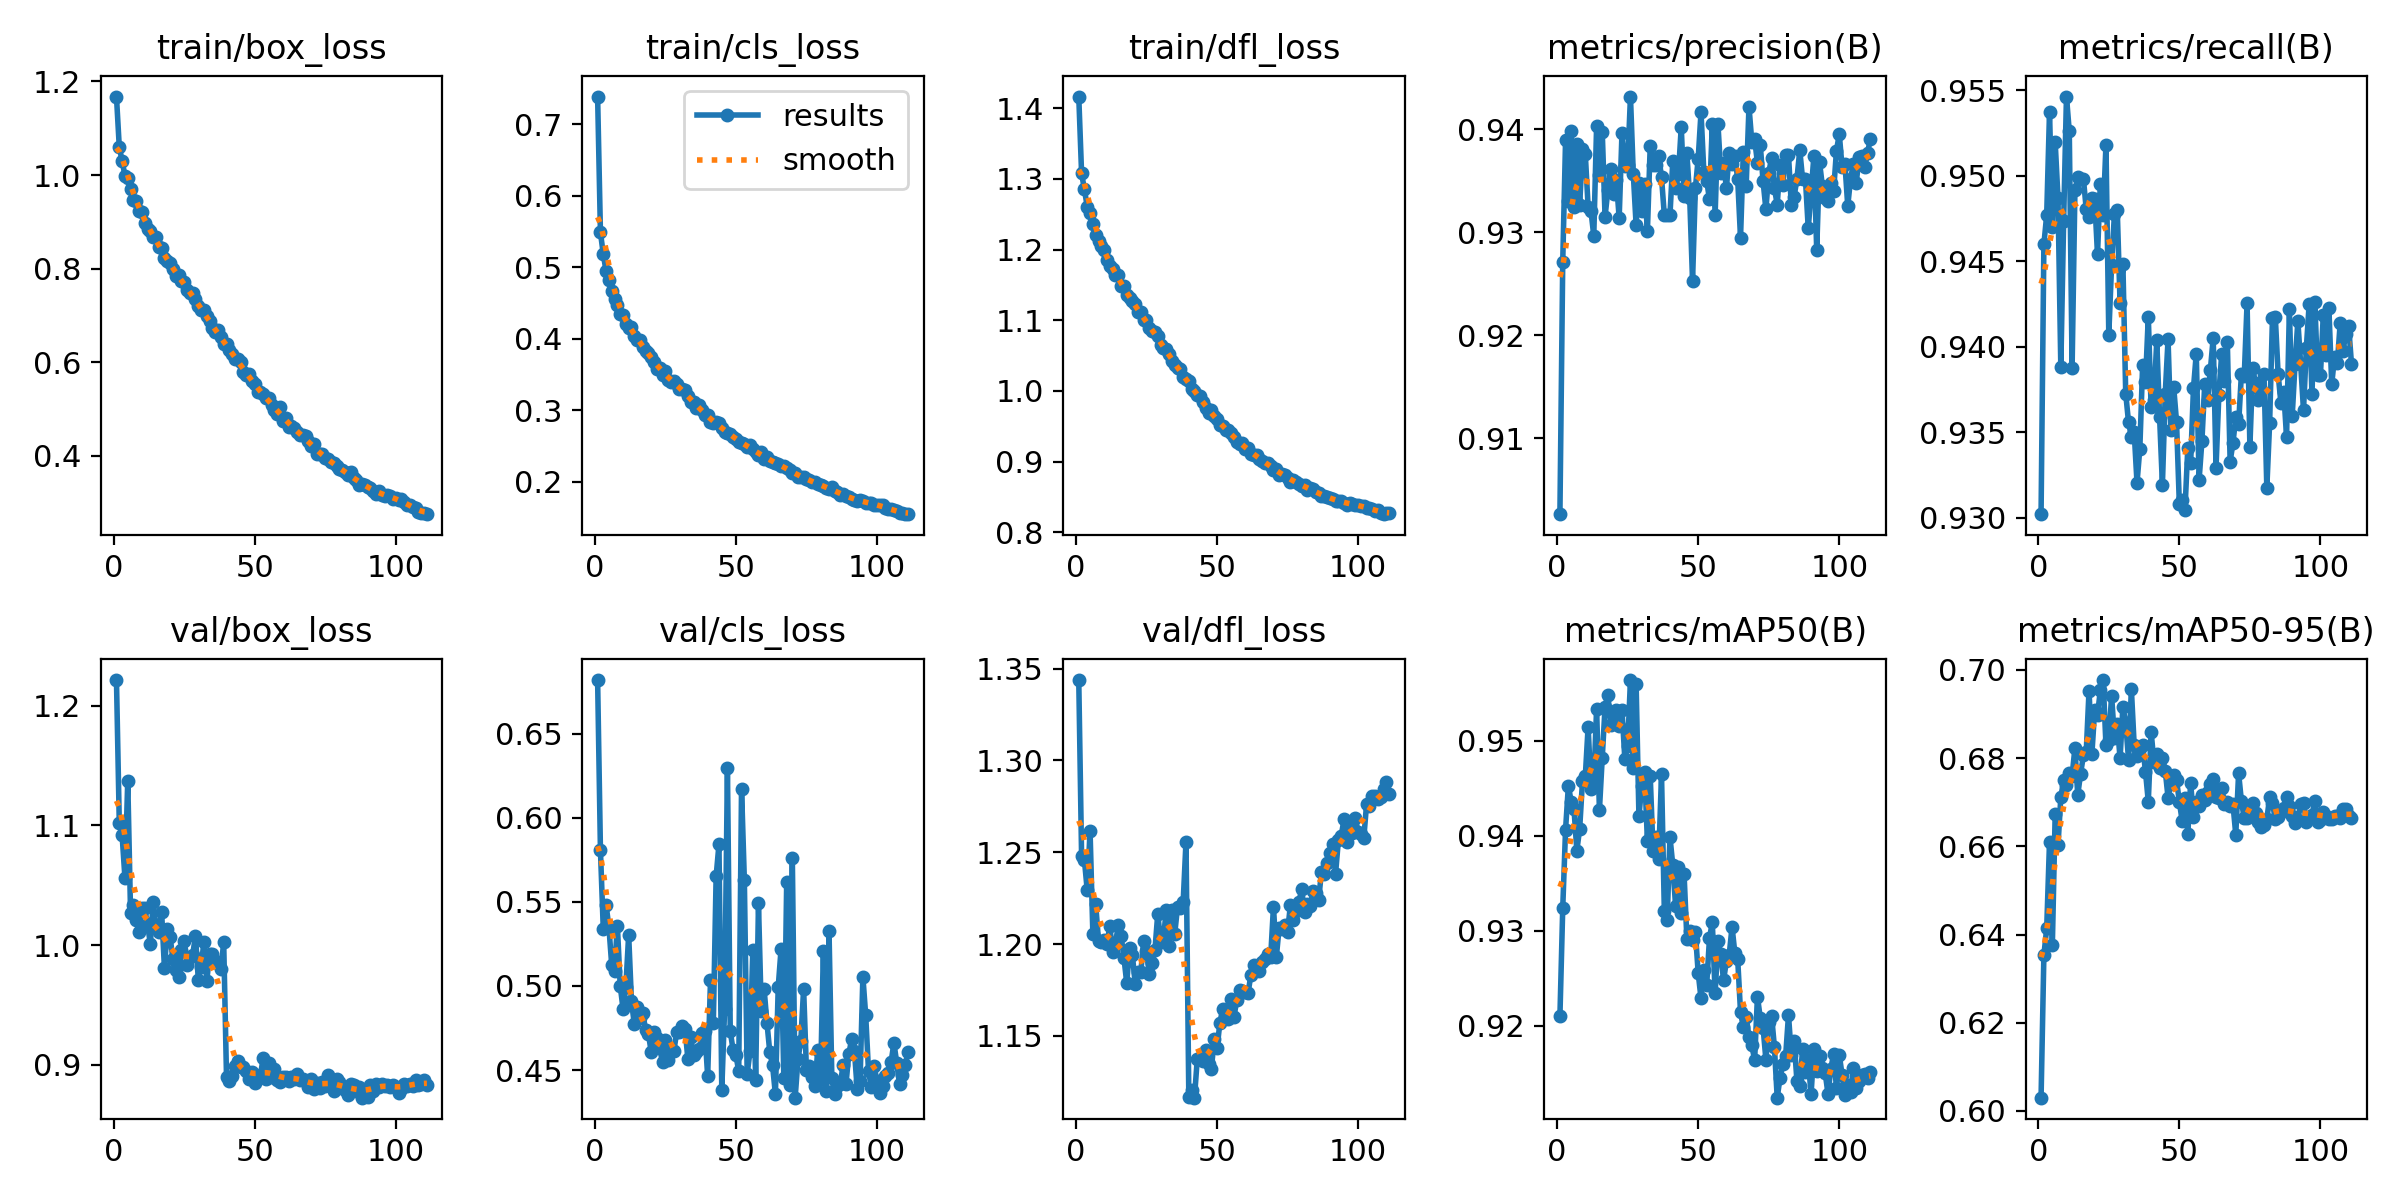
\includegraphics[width=\textwidth]{images/image_ch3/results_recto/results.png}
  \caption{Évolution des pertes et métriques d'entraînement --- CIN Recto}
  \label{fig:ch3-results-recto}
\end{figure}

La Figure~\ref{fig:ch3-results-recto} montre une convergence progressive des pertes d'entraînement et de validation, avec une mAP50 qui atteint 0,953 en fin d'entraînement. Le mAP50-95 global de 0,698 traduit une localisation précise des bounding boxes, ce qui est cohérent avec la complexité du recto --- 10 classes dont plusieurs champs compacts (\texttt{num\_cin}, \texttt{dob}).

\begin{figure}[H]
  \centering
  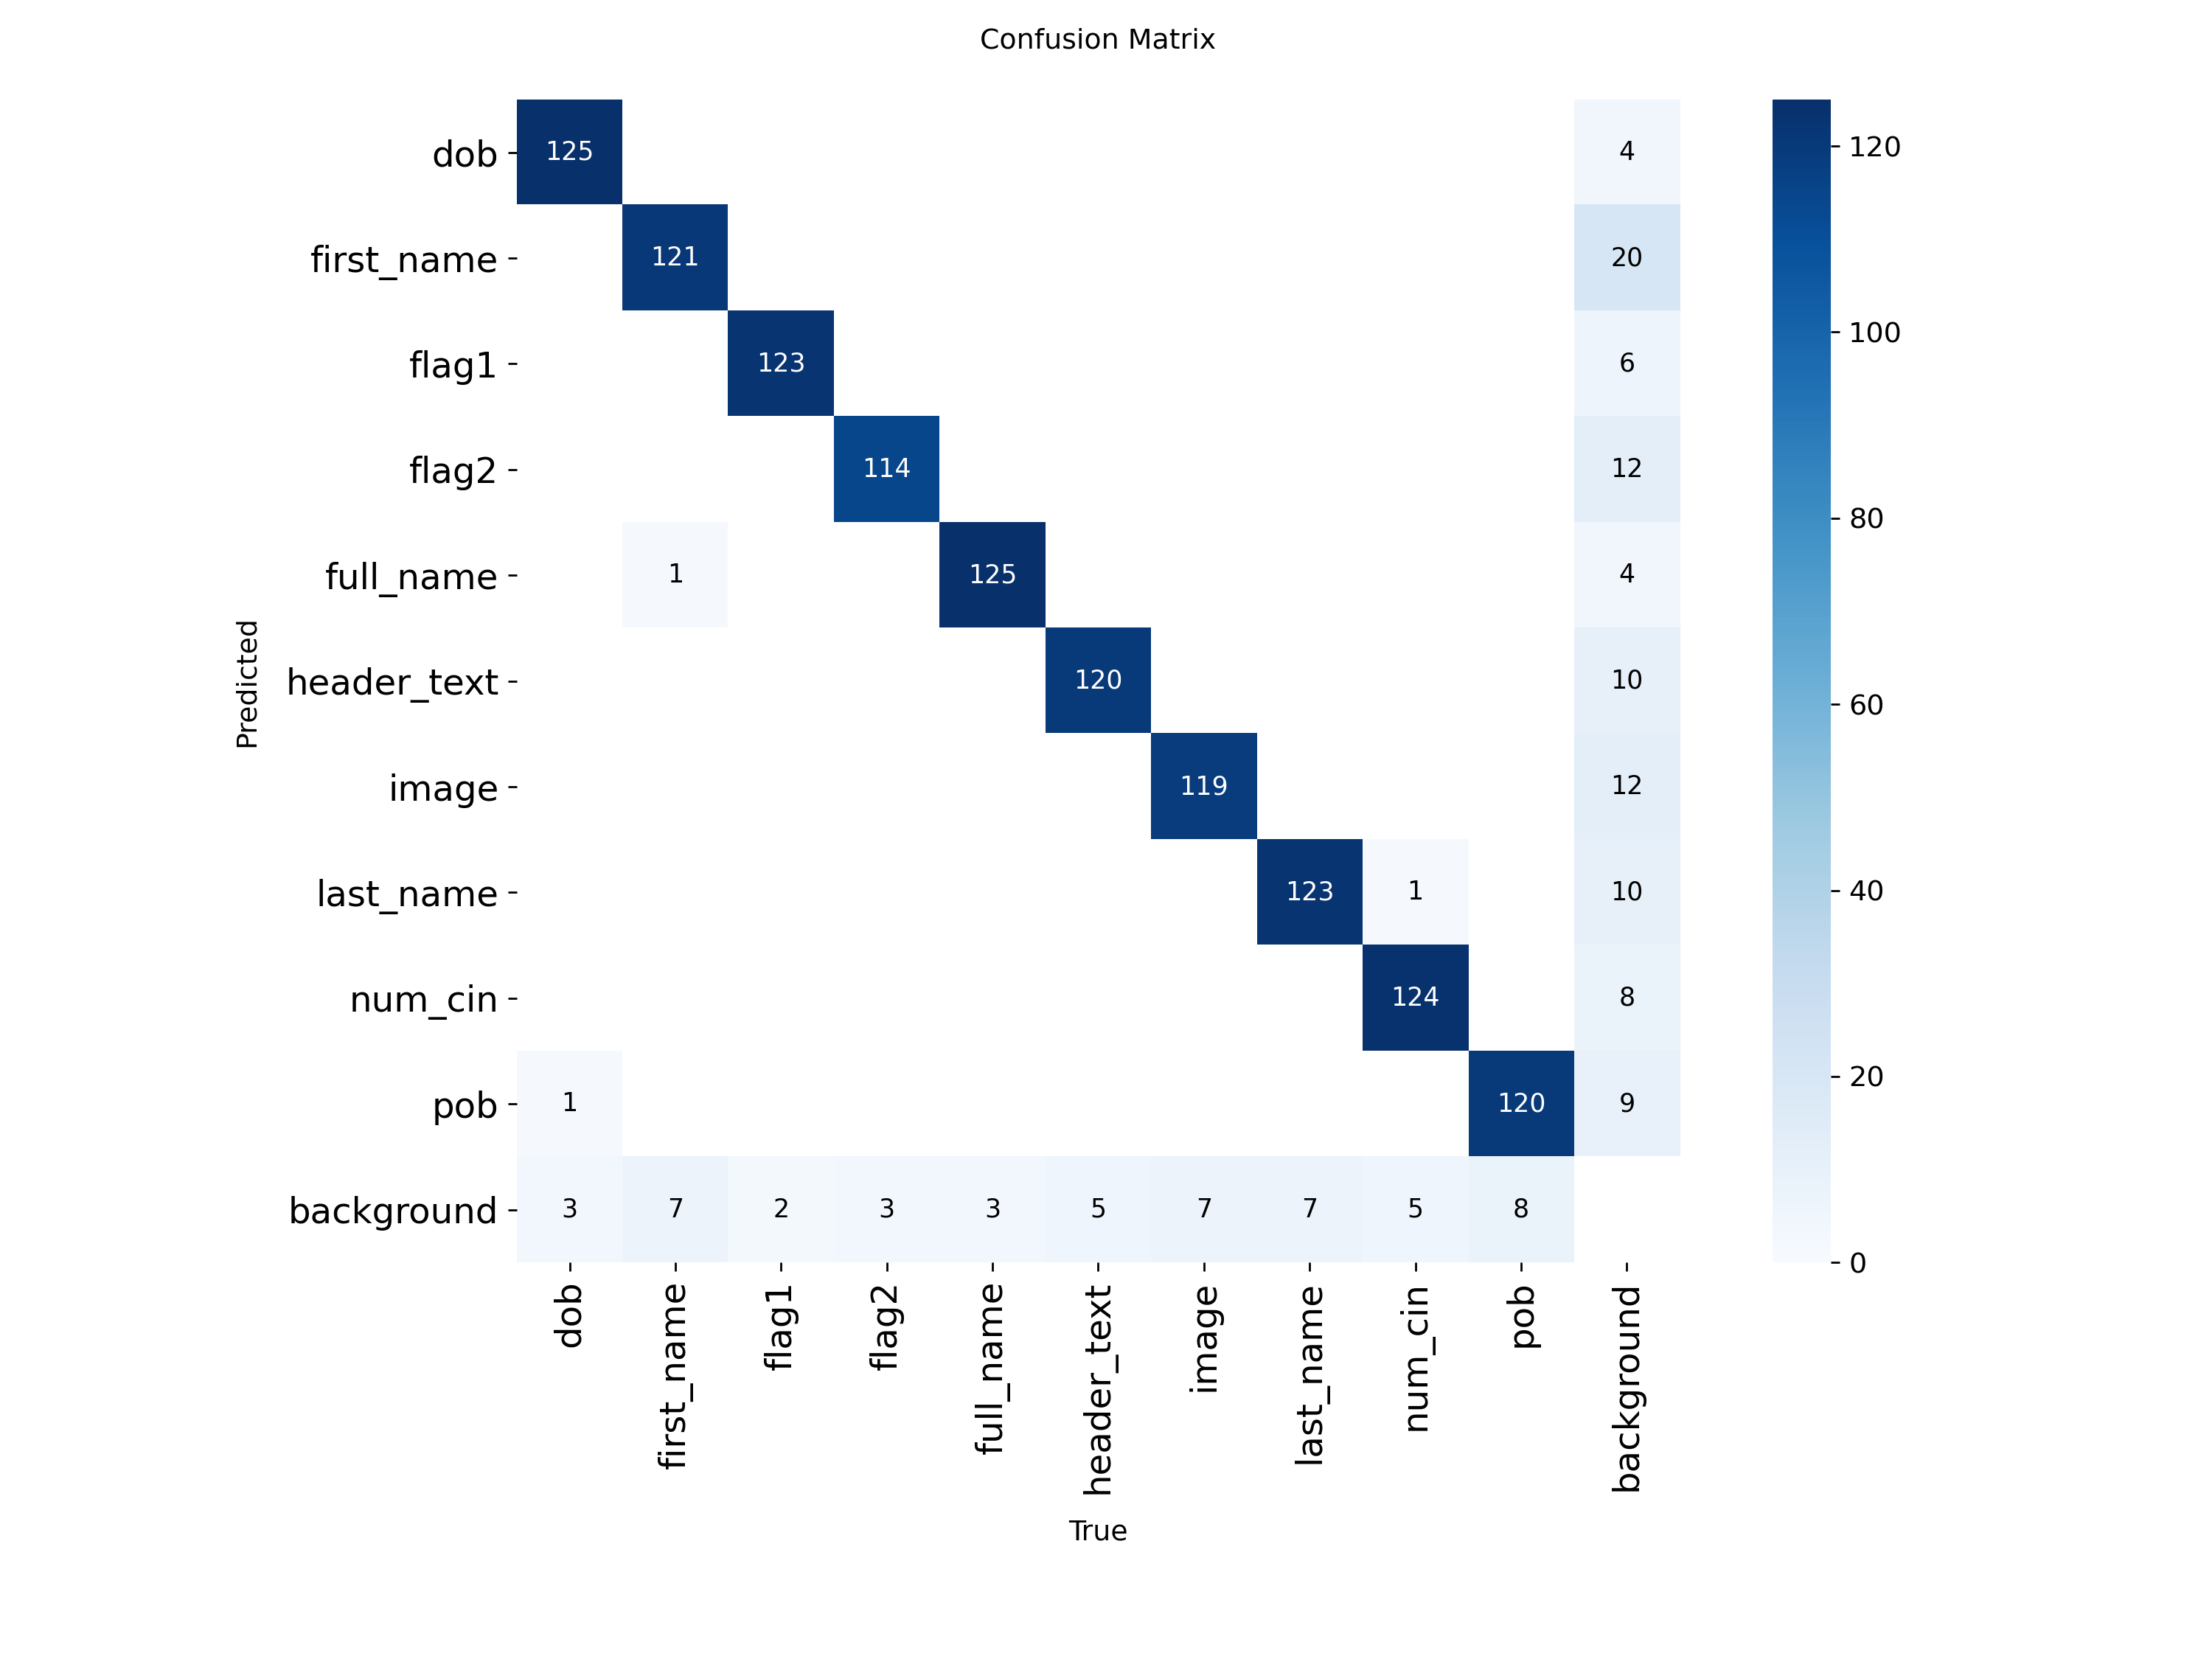
\includegraphics[width=0.80\textwidth]{images/image_ch3/results_recto/confusion_matrix.png}
  \caption{Matrice de confusion --- CIN Recto}
  \label{fig:ch3-cm-recto}
\end{figure}

La matrice de confusion (Figure~\ref{fig:ch3-cm-recto}) confirme la solidité du modèle sur les classes structurées (\texttt{flag1}, \texttt{flag2}, \texttt{num\_cin}). Les confusions les plus notables concernent \texttt{first\_name} et \texttt{pob}, dont la position et la typographie sont proches sur le document.

Le Tableau~\ref{tab:ch3-metrics-recto} présente les métriques détaillées par champ, évaluées sur le jeu de validation (156 images, 1\,267 instances).

\begin{table}[H]
  \centering
  \small
  \begin{tabular}{|l|c|c|c|c|}
    \toprule
    \rowcolor{bleu_principal}
    \textcolor{white}{\textbf{Champ}} & \textcolor{white}{\textbf{Précision}} & \textcolor{white}{\textbf{Rappel}} & \textcolor{white}{\textbf{mAP50}} & \textcolor{white}{\textbf{mAP50-95}} \\
    \midrule
    \texttt{dob}         & 0,973 & 0,969 & 0,963 & 0,649 \\
    \midrule
    \rowcolor{gris_leger}
    \texttt{first\_name} & 0,920 & 0,896 & 0,917 & 0,569 \\
    \midrule
    \texttt{flag1}       & 0,951 & 0,984 & 0,983 & 0,820 \\
    \midrule
    \rowcolor{gris_leger}
    \texttt{flag2}       & 0,924 & 0,940 & 0,976 & 0,815 \\
    \midrule
    \texttt{full\_name}  & 0,961 & 0,971 & 0,970 & 0,645 \\
    \midrule
    \rowcolor{gris_leger}
    \texttt{header\_text}& 0,920 & 0,960 & 0,938 & 0,831 \\
    \midrule
    \texttt{image}       & 0,919 & 0,944 & 0,924 & 0,769 \\
    \midrule
    \rowcolor{gris_leger}
    \texttt{last\_name}  & 0,946 & 0,937 & 0,952 & 0,626 \\
    \midrule
    \texttt{num\_cin}    & 0,956 & 0,954 & 0,969 & 0,667 \\
    \midrule
    \rowcolor{gris_leger}
    \texttt{pob}         & 0,926 & 0,922 & 0,939 & 0,591 \\
    \midrule
    \rowcolor{bleu_clair!15}
    \textbf{Global}      & \textbf{0,940} & \textbf{0,948} & \textbf{0,953} & \textbf{0,698} \\
    \bottomrule
  \end{tabular}
  \caption{Métriques de validation par champ --- modèle CIN Recto}
  \label{tab:ch3-metrics-recto}
\end{table}

\paragraph{CIN Verso}

\begin{figure}[H]
  \centering
  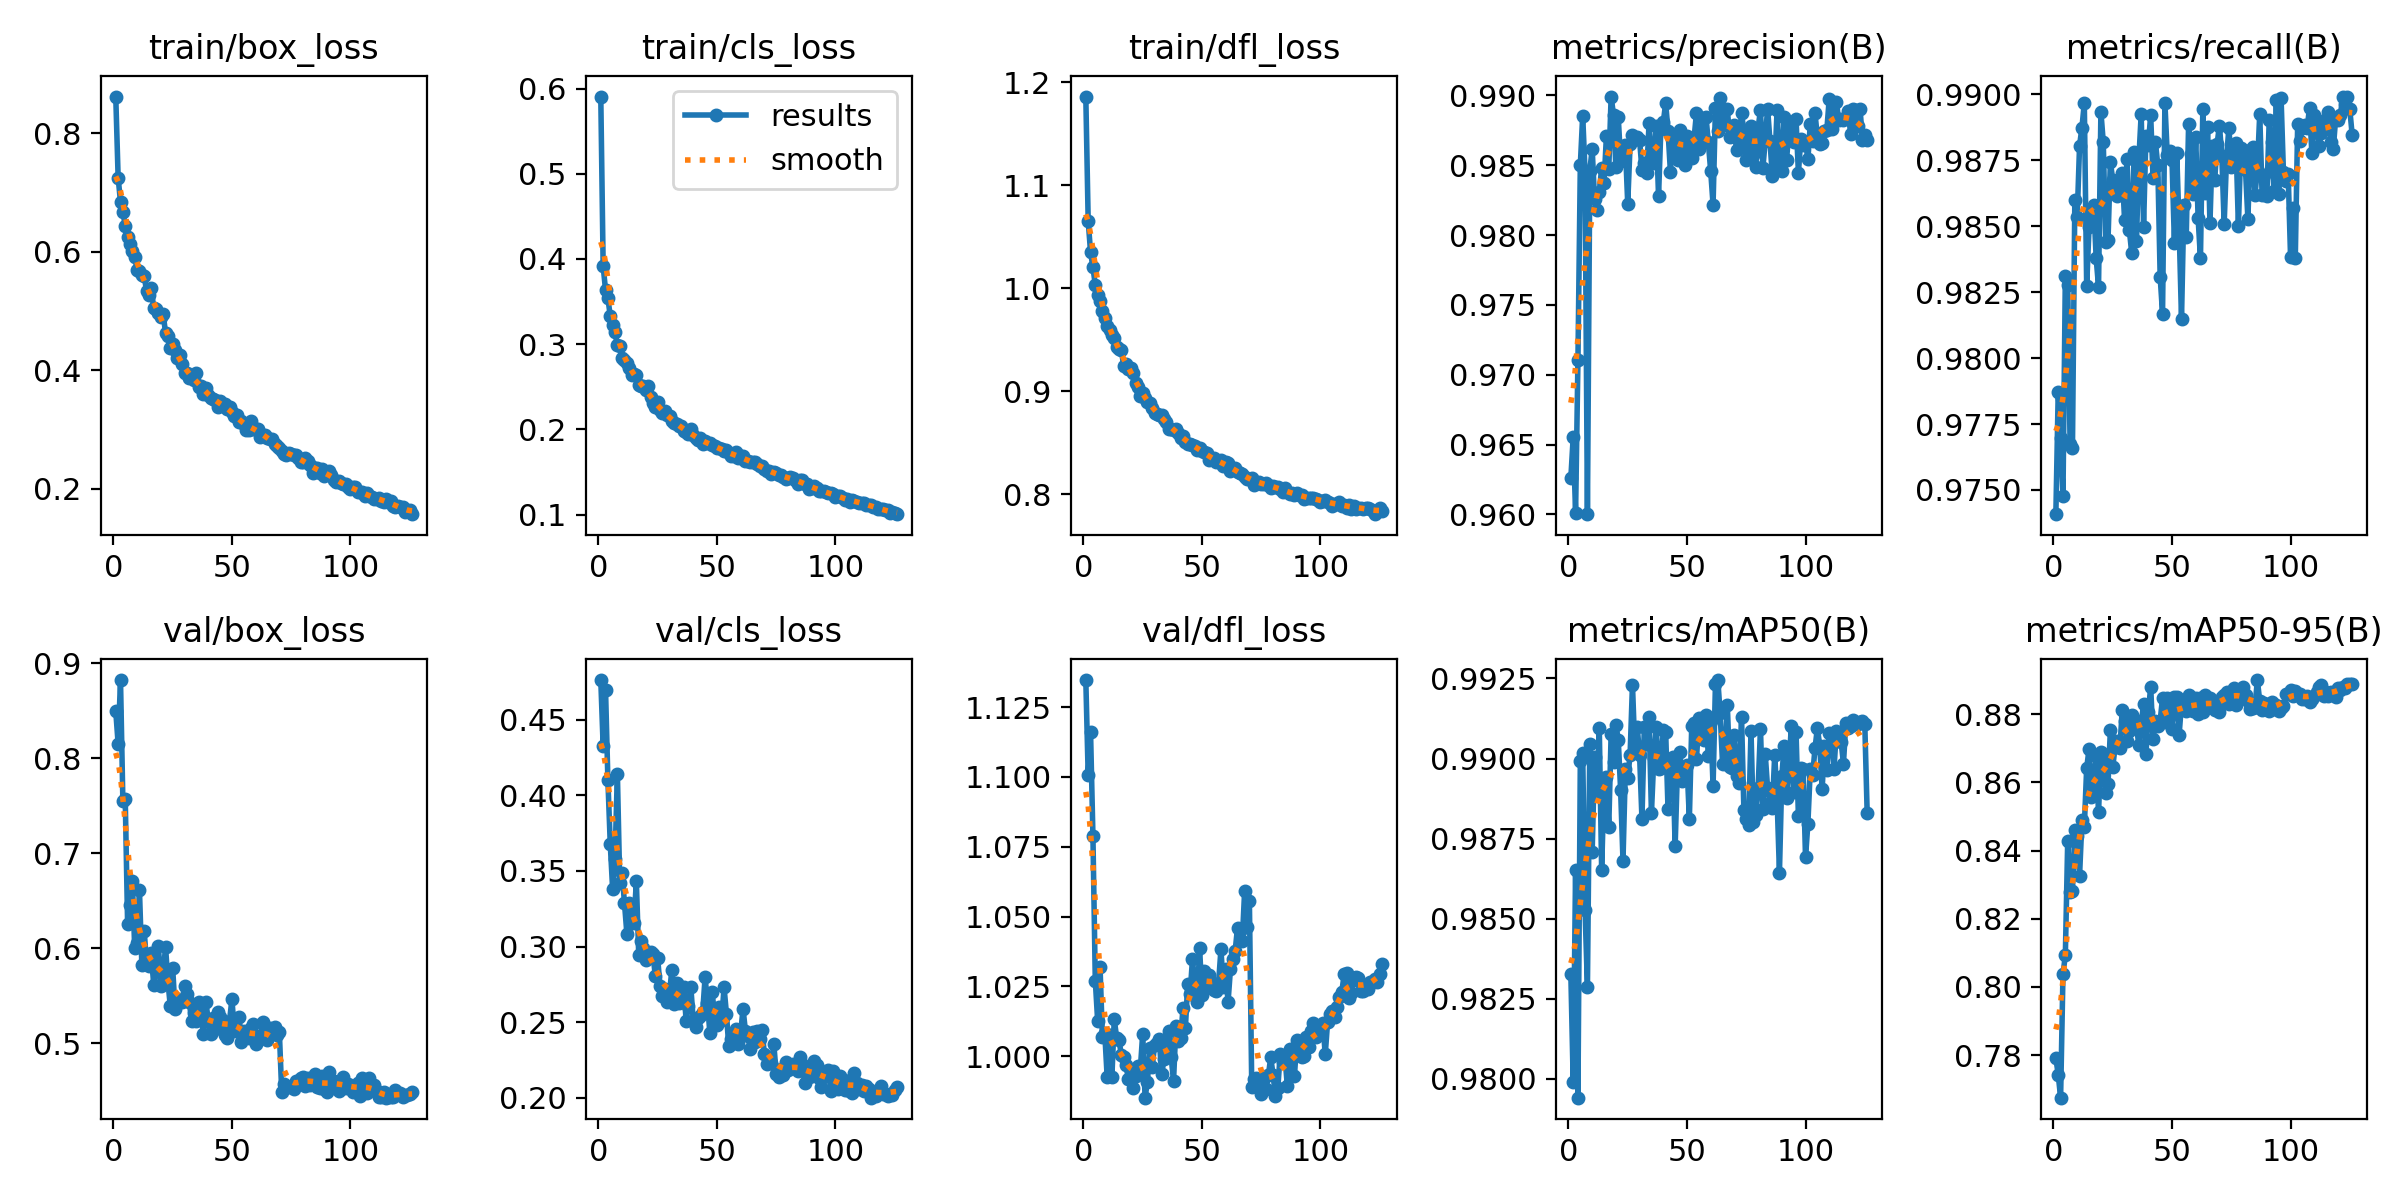
\includegraphics[width=\textwidth]{images/image_ch3/results_verso/results.png}
  \caption{Évolution des pertes et métriques d'entraînement --- CIN Verso}
  \label{fig:ch3-results-verso}
\end{figure}

La Figure~\ref{fig:ch3-results-verso} montre une convergence rapide des trois composantes de perte (box, cls, dfl) dès les 50 premières époques, avec une mAP50 qui se stabilise autour de 0,988 en fin d'entraînement.

\begin{figure}[H]
  \centering
  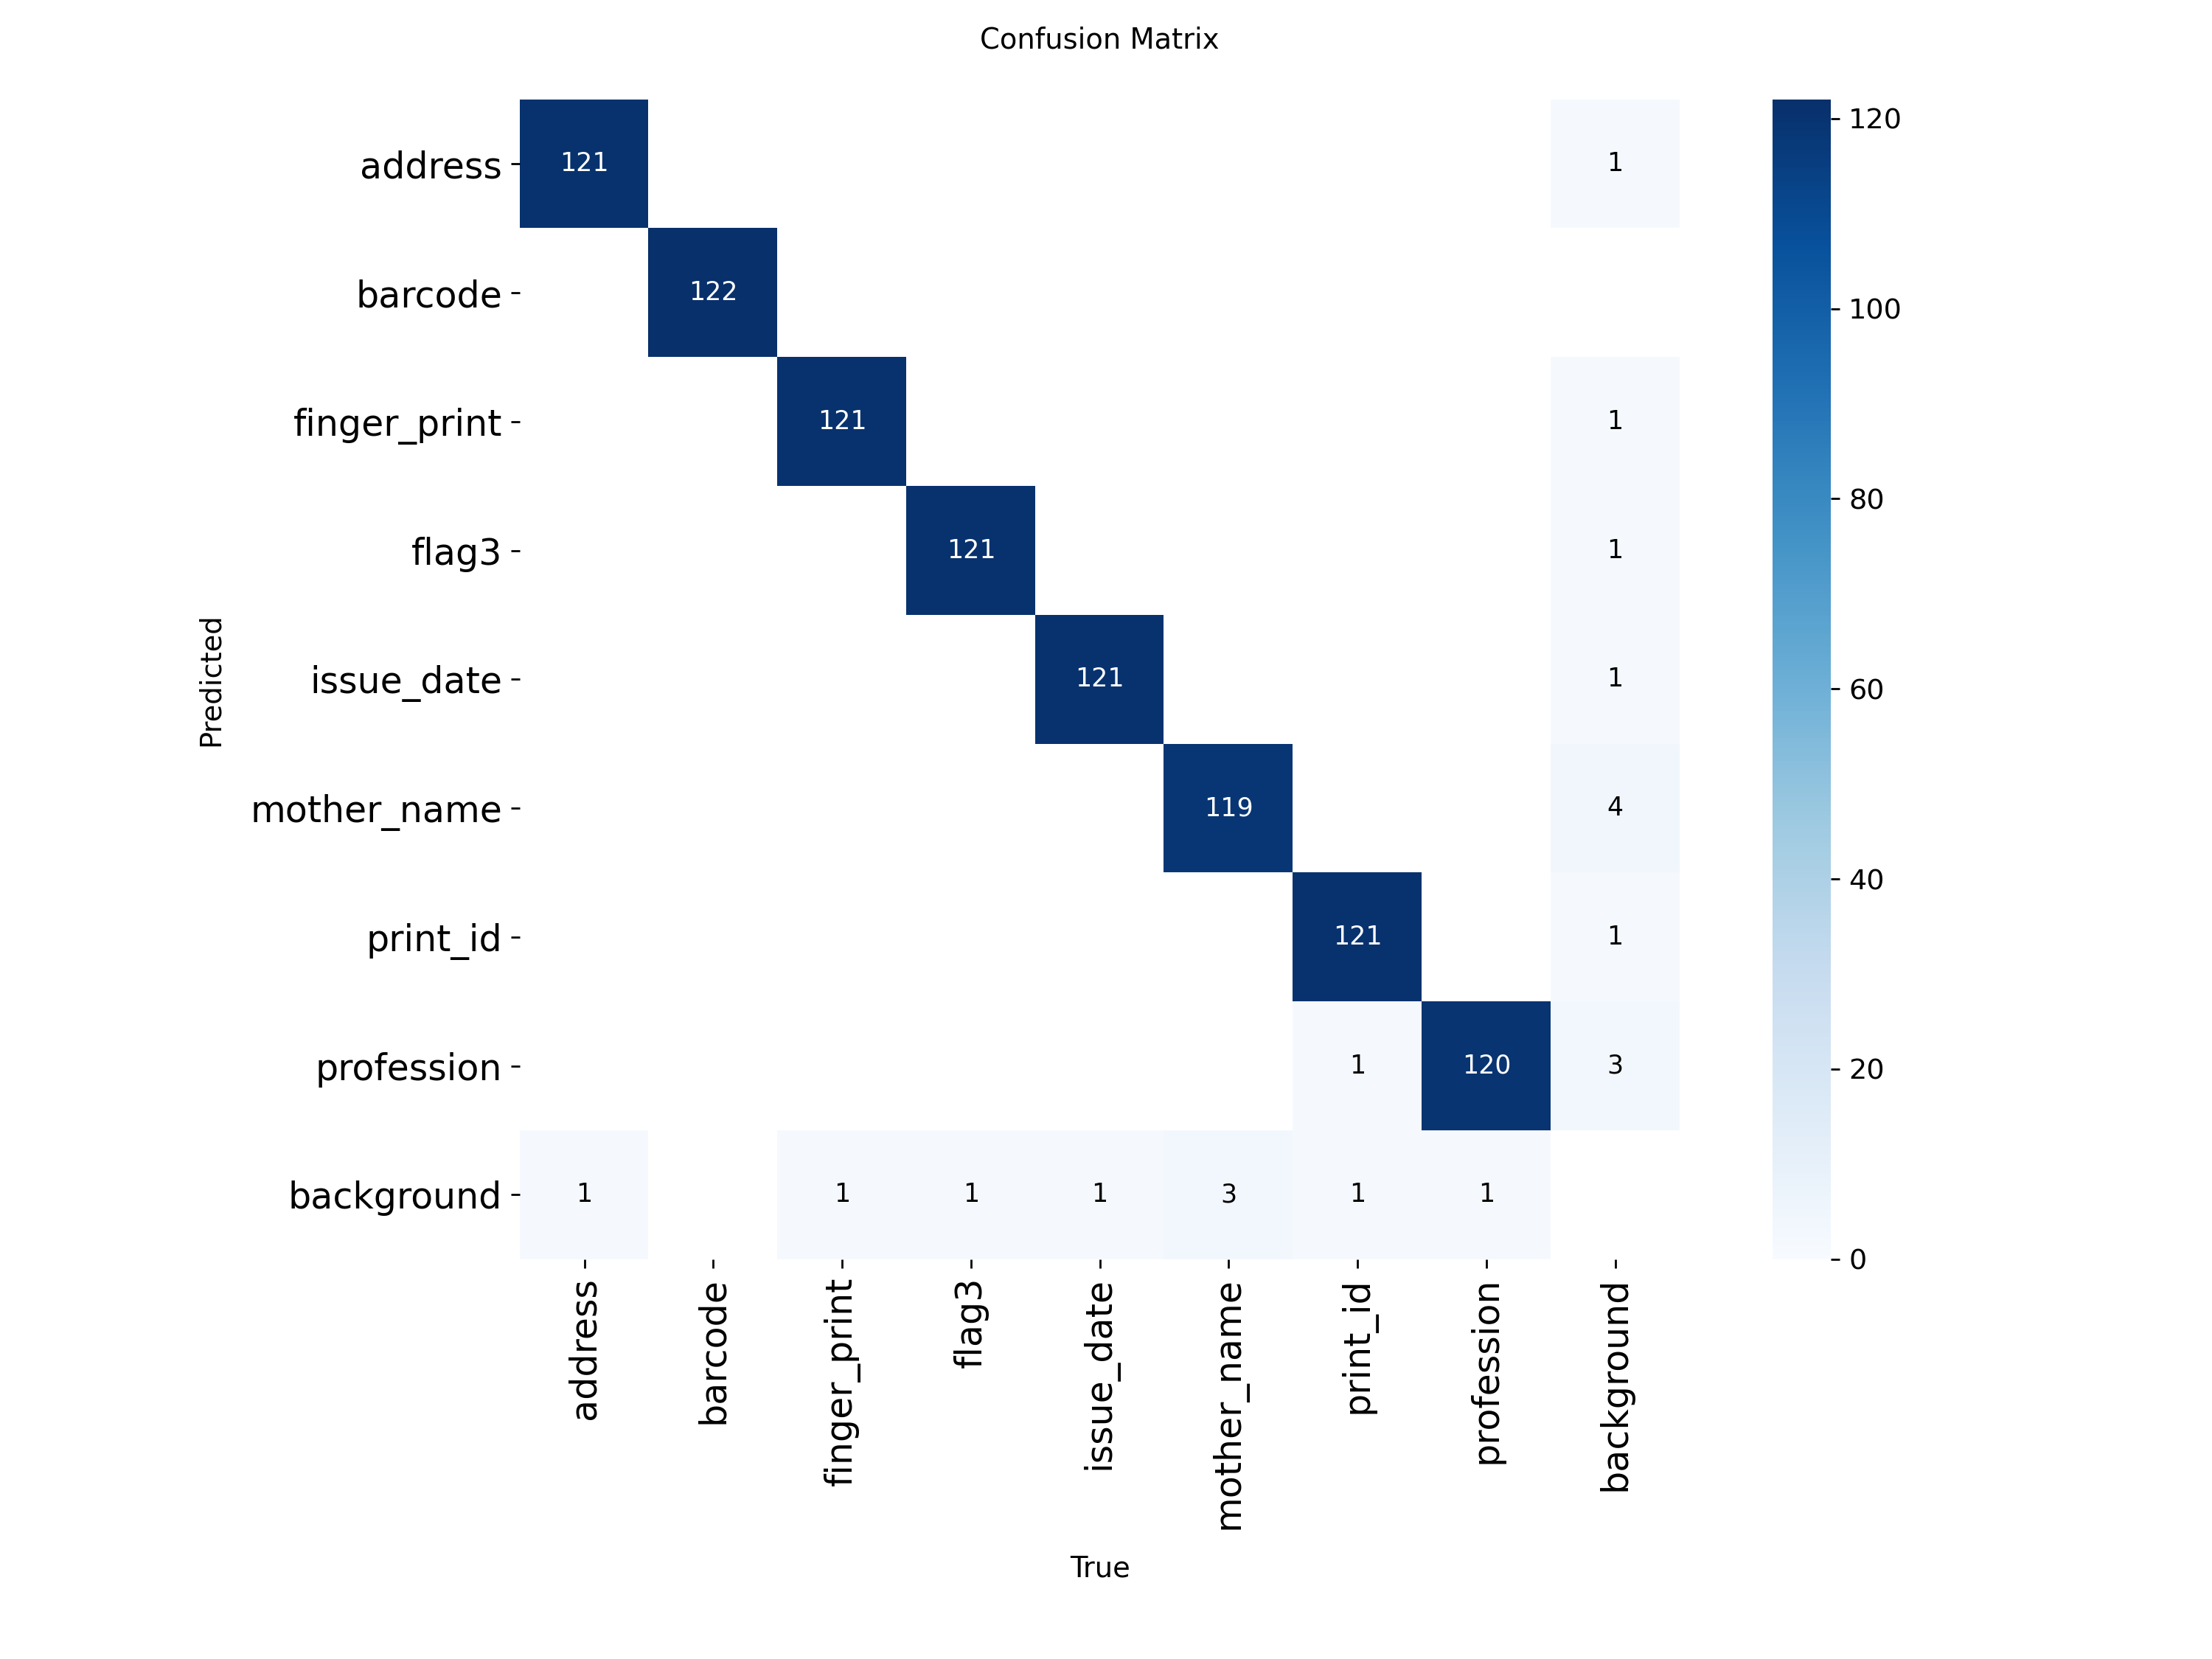
\includegraphics[width=0.80\textwidth]{images/image_ch3/results_verso/confusion_matrix.png}
  \caption{Matrice de confusion --- CIN Verso}
  \label{fig:ch3-cm-verso}
\end{figure}

La matrice de confusion (Figure~\ref{fig:ch3-cm-verso}) révèle que la quasi-totalité des 8 classes sont correctement localisées. Le champ \texttt{mother\_name} présente le plus grand nombre de confusions (4 instances classées en arrière-plan), ce qui s'explique par sa position variable sur le document et la similitude visuelle avec le champ \texttt{profession}.

Le Tableau~\ref{tab:ch3-metrics-verso} présente les métriques détaillées par champ, telles qu'évaluées sur le jeu de validation (148 images, 976 instances).

\begin{table}[H]
  \centering
  \small
  \begin{tabular}{|l|c|c|c|c|}
    \toprule
    \rowcolor{bleu_principal}
    \textcolor{white}{\textbf{Champ}} & \textcolor{white}{\textbf{Précision}} & \textcolor{white}{\textbf{Rappel}} & \textcolor{white}{\textbf{mAP50}} & \textcolor{white}{\textbf{mAP50-95}} \\
    \midrule
    \texttt{address}      & 0,988 & 0,992 & 0,992 & 0,863 \\
    \midrule
    \rowcolor{gris_leger}
    \texttt{barcode}      & 1,000 & 1,000 & 0,995 & 0,969 \\
    \midrule
    \texttt{finger\_print} & 0,988 & 0,992 & 0,994 & 0,976 \\
    \midrule
    \rowcolor{gris_leger}
    \texttt{flag3}        & 0,992 & 0,992 & 0,995 & 0,953 \\
    \midrule
    \texttt{issue\_date}  & 0,992 & 0,990 & 0,994 & 0,928 \\
    \midrule
    \rowcolor{gris_leger}
    \texttt{mother\_name} & 0,952 & 0,959 & 0,961 & 0,792 \\
    \midrule
    \texttt{print\_id}    & 0,987 & 0,984 & 0,984 & 0,903 \\
    \midrule
    \rowcolor{gris_leger}
    \texttt{profession}   & 0,976 & 0,990 & 0,992 & 0,738 \\
    \midrule
    \rowcolor{bleu_clair!15}
    \textbf{Global}       & \textbf{0,984} & \textbf{0,987} & \textbf{0,988} & \textbf{0,890} \\
    \bottomrule
  \end{tabular}
  \caption{Métriques de validation par champ --- modèle CIN Verso}
  \label{tab:ch3-metrics-verso}
\end{table}

\paragraph{Passeport}

\begin{figure}[H]
  \centering
  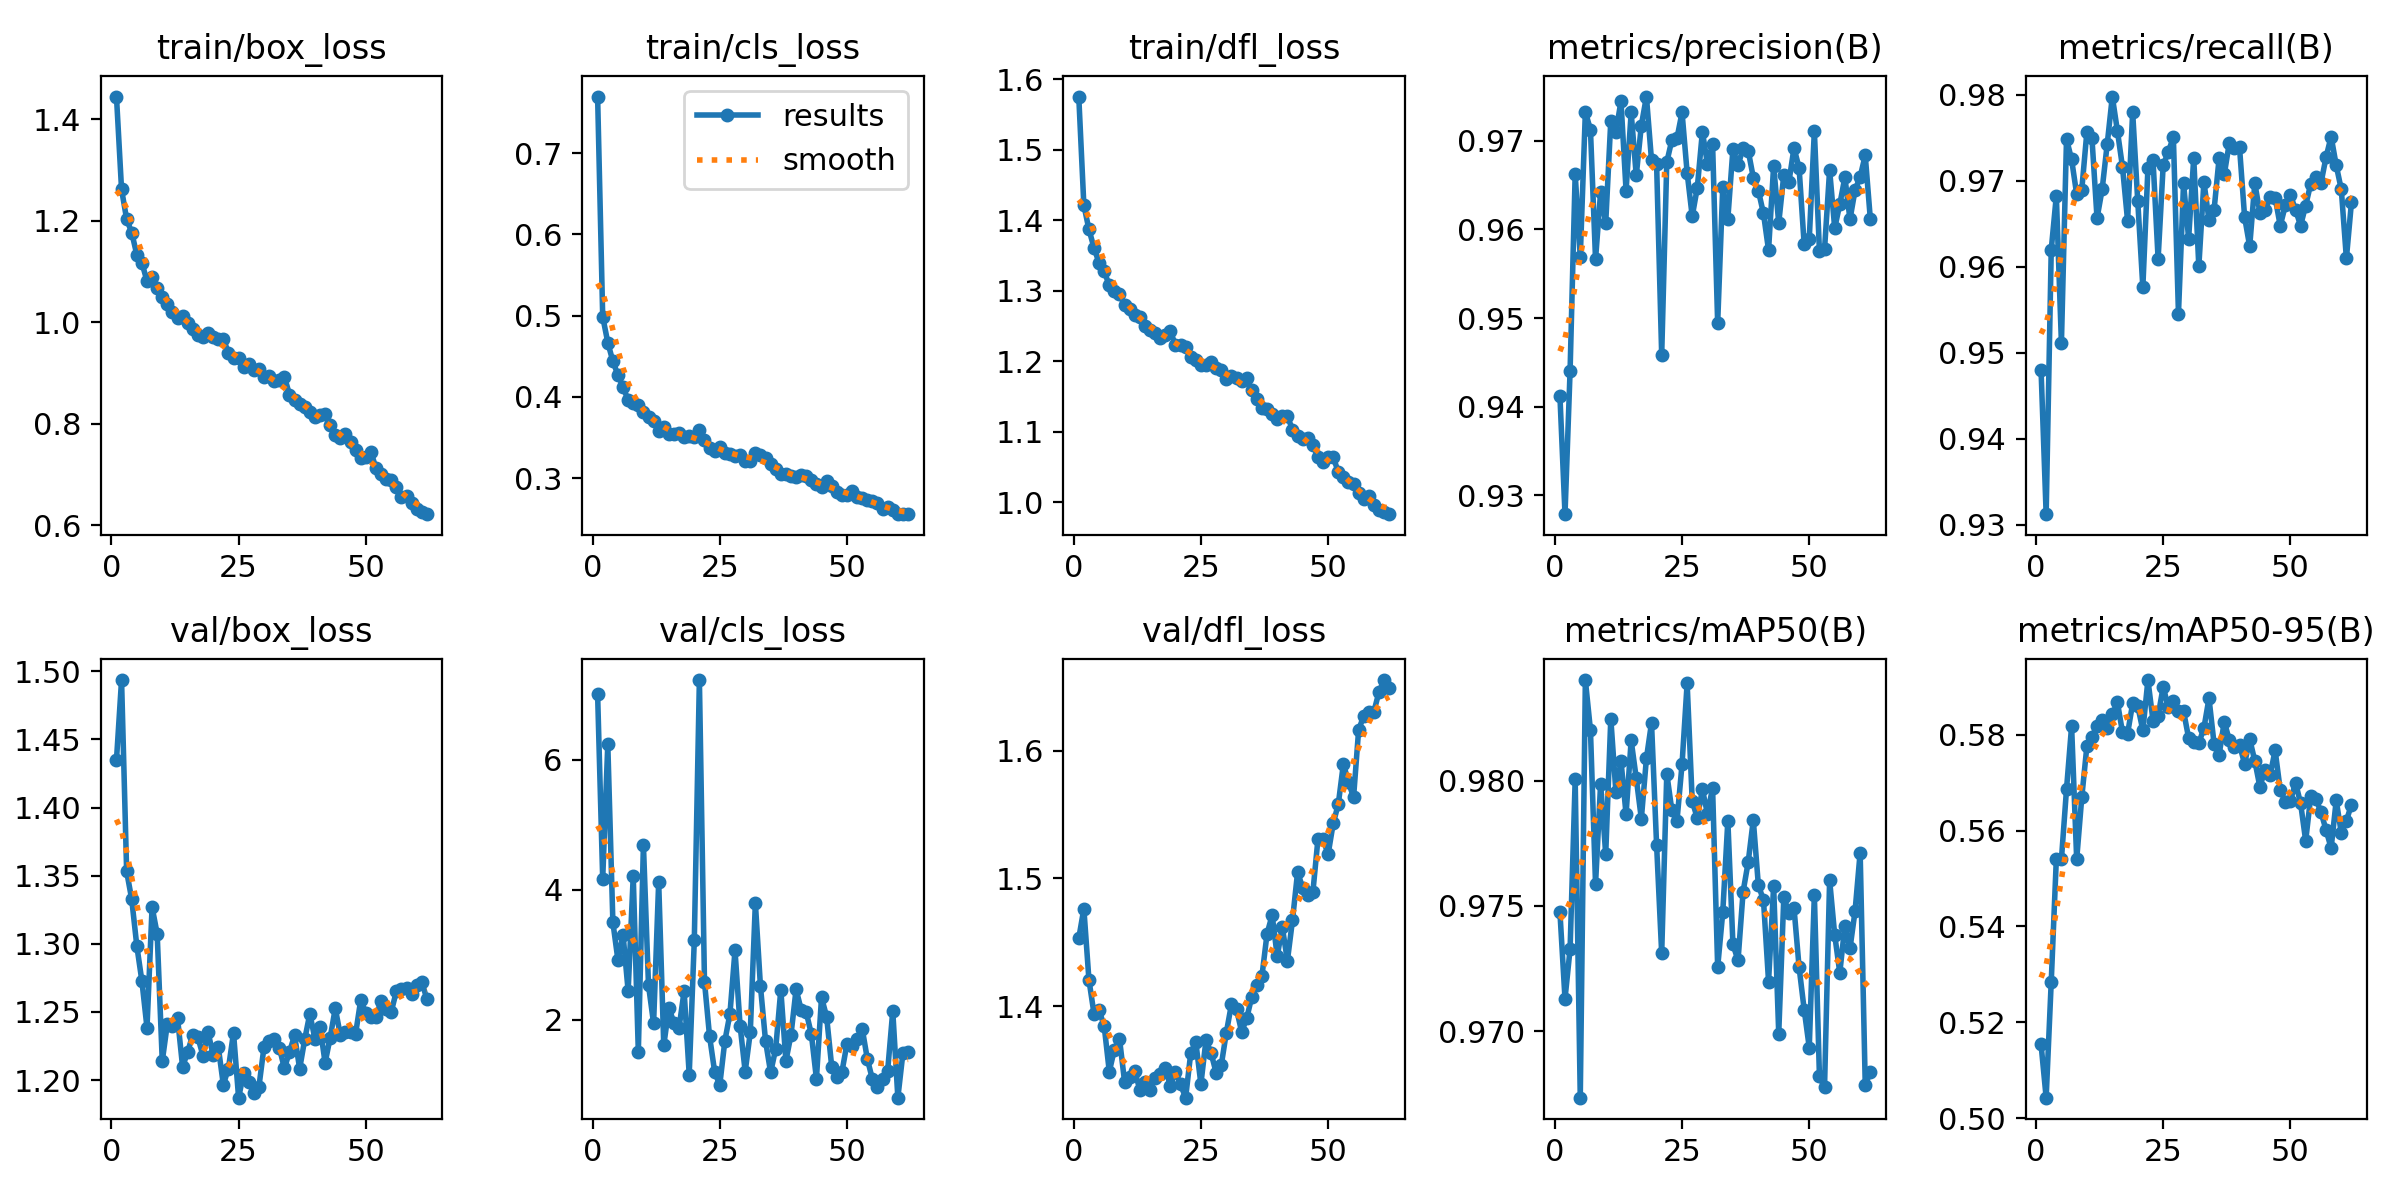
\includegraphics[width=\textwidth]{images/image_ch3/results_passport/results.png}
  \caption{Évolution des pertes et métriques d'entraînement --- Passeport}
  \label{fig:ch3-results-passport}
\end{figure}

La Figure~\ref{fig:ch3-results-passport} illustre une convergence stable, avec une mAP50 finale de 0,980. Le mAP50-95 global de 0,592 est plus bas que pour la CIN, ce qui s'explique par la densité textuelle élevée du passeport (12 classes dont plusieurs champs proches comme \texttt{first\_name}, \texttt{last\_name} et \texttt{full\_name}) et un dataset plus réduit (137 images de validation).

\begin{figure}[H]
  \centering
  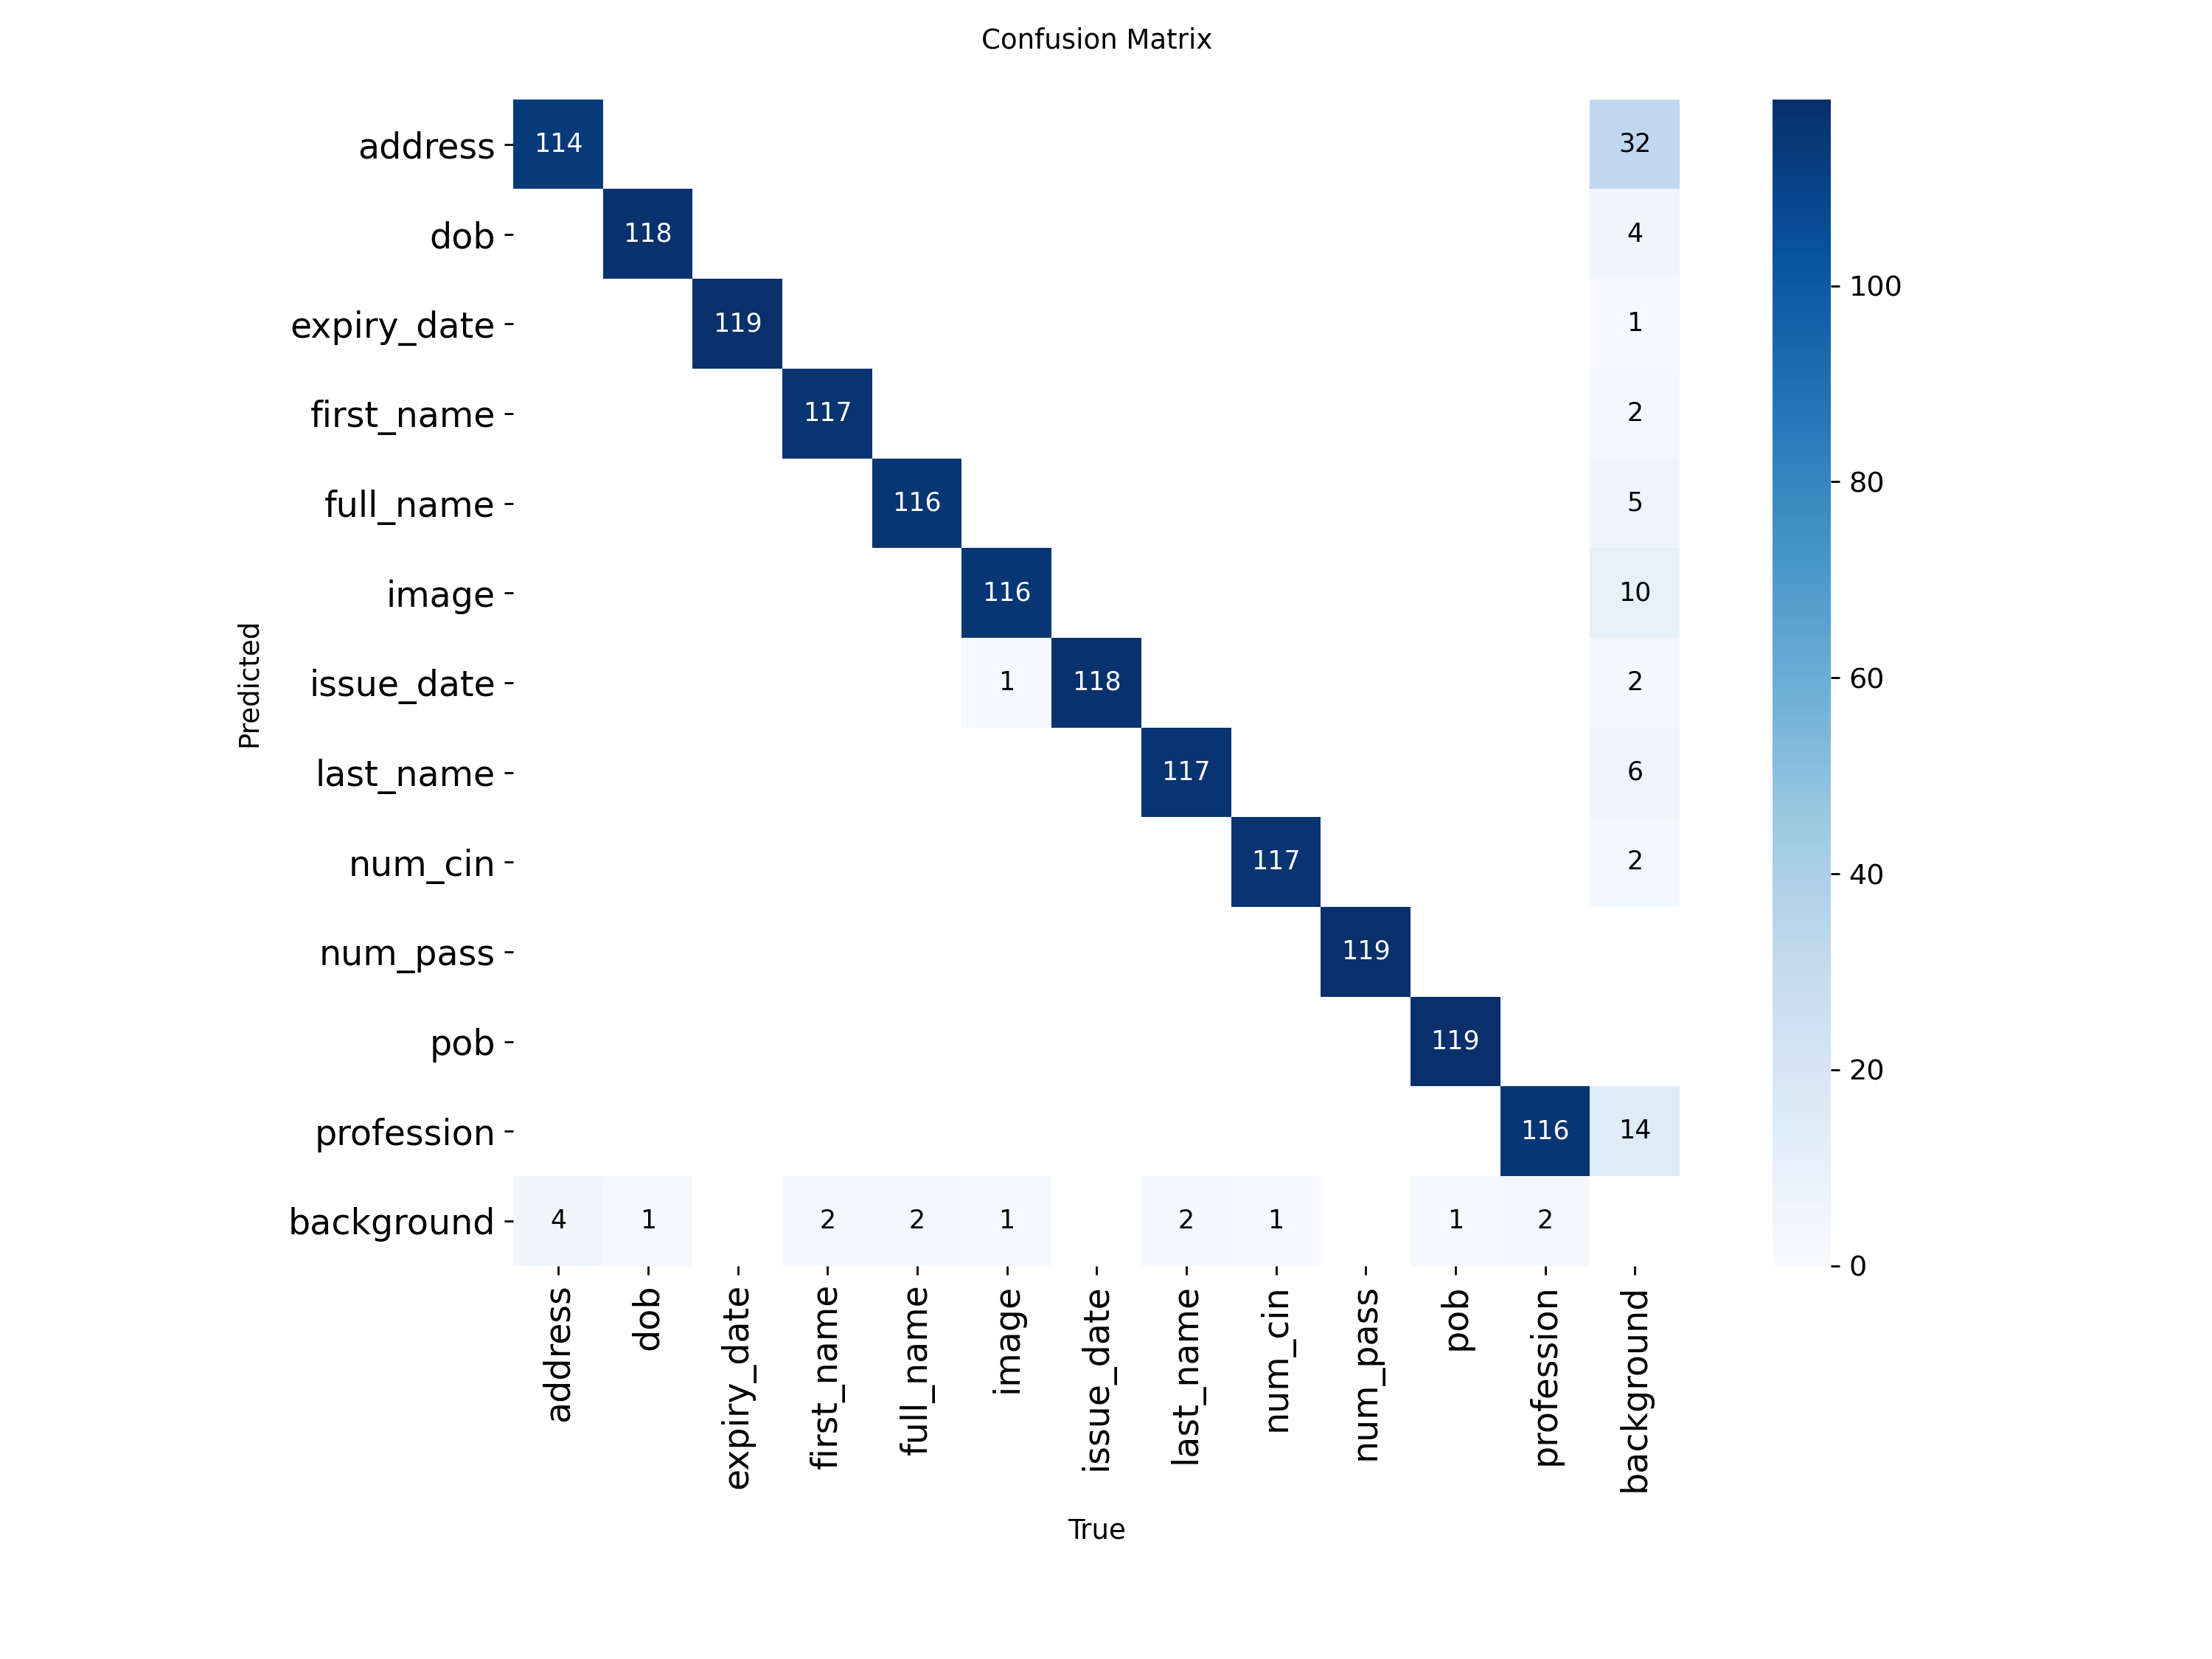
\includegraphics[width=0.80\textwidth]{images/image_ch3/results_passport/confusion_matrix.png}
  \caption{Matrice de confusion --- Passeport}
  \label{fig:ch3-cm-passport}
\end{figure}

La matrice de confusion (Figure~\ref{fig:ch3-cm-passport}) confirme d'excellentes performances sur les champs structurés (\texttt{num\_pass}, \texttt{pob}, \texttt{image}). Le champ \texttt{address} présente le rappel le plus bas (0,856), attribuable à sa position variable selon les versions du passeport tunisien.

Le Tableau~\ref{tab:ch3-metrics-passport} présente les métriques détaillées par champ, évaluées sur le jeu de validation (137 images, 1\,423 instances).

\begin{table}[H]
  \centering
  \small
  \begin{tabular}{|l|c|c|c|c|}
    \toprule
    \rowcolor{bleu_principal}
    \textcolor{white}{\textbf{Champ}} & \textcolor{white}{\textbf{Précision}} & \textcolor{white}{\textbf{Rappel}} & \textcolor{white}{\textbf{mAP50}} & \textcolor{white}{\textbf{mAP50-95}} \\
    \midrule
    \texttt{address}     & 0,936 & 0,856 & 0,950 & 0,540 \\
    \midrule
    \rowcolor{gris_leger}
    \texttt{dob}         & 0,963 & 0,975 & 0,982 & 0,599 \\
    \midrule
    \texttt{expiry\_date}& 0,992 & 0,995 & 0,995 & 0,583 \\
    \midrule
    \rowcolor{gris_leger}
    \texttt{first\_name} & 0,974 & 0,963 & 0,950 & 0,512 \\
    \midrule
    \texttt{full\_name}  & 0,976 & 0,975 & 0,989 & 0,664 \\
    \midrule
    \rowcolor{gris_leger}
    \texttt{image}       & 0,943 & 0,988 & 0,992 & 0,840 \\
    \midrule
    \texttt{issue\_date} & 0,975 & 0,983 & 0,971 & 0,565 \\
    \midrule
    \rowcolor{gris_leger}
    \texttt{last\_name}  & 0,958 & 0,983 & 0,976 & 0,569 \\
    \midrule
    \texttt{num\_cin}    & 0,983 & 0,992 & 0,992 & 0,572 \\
    \midrule
    \rowcolor{gris_leger}
    \texttt{num\_pass}   & 0,999 & 1,000 & 0,995 & 0,544 \\
    \midrule
    \texttt{pob}         & 0,997 & 0,992 & 0,995 & 0,609 \\
    \midrule
    \rowcolor{gris_leger}
    \texttt{profession}  & 0,923 & 0,958 & 0,979 & 0,501 \\
    \midrule
    \rowcolor{bleu_clair!15}
    \textbf{Global}      & \textbf{0,968} & \textbf{0,971} & \textbf{0,980} & \textbf{0,592} \\
    \bottomrule
  \end{tabular}
  \caption{Métriques de validation par champ --- modèle Passeport}
  \label{tab:ch3-metrics-passport}
\end{table}

%-------------------------------------------------------------
\subsection{Extraction texte --- PaddleOCR PP-OCRv5}
\label{subsec:paddleocr-extraction}
%-------------------------------------------------------------

Comme présenté au chapitre 2, PP-OCRv5 a été retenu pour ses performances sur les scripts arabes et latins simultanément, sa légèreté et sa compatibilité avec un déploiement \textit{on-premise}. Dans le pipeline, il reçoit en entrée les crops produits par YOLOv11m et retourne le texte structuré de chaque champ.

\subsubsection*{Workflow d'extraction}

Le pipeline d'extraction suit quatre étapes enchaînées pour chaque zone détectée par YOLO :

\begin{enumerate}
  \item \textbf{Recadrage (crop)} : la bounding box YOLO est appliquée à l'image haute résolution. Des ajustements fins compensent les légères sous-détections :
  \begin{itemize}
    \item Élargissement des bords pour les dates du passeport.
    \item Réduction à droite pour l'adresse verso (exclure le label « العنوان » imprimé).
    \item Conservation des trois quarts supérieurs pour le champ nom recto.
  \end{itemize}

  \item \textbf{Prétraitement (preprocessing)} : plusieurs traitements sont appliqués selon la qualité du crop :
  \begin{itemize}
    \item Ajout d'une bordure blanche de 40 pixels sur chaque côté.
    \item Si hauteur $<$ 80 px : agrandissement par interpolation Lanczos4.
    \item Pour les champs sur fond texturé : binarisation adaptative pour séparer texte et fond.
  \end{itemize}

  \item \textbf{Lecture OCR} : deux moteurs fonctionnent en parallèle selon la langue du champ :
  \begin{itemize}
    \item Moteur arabe : champs identitaires (nom, prénom, adresse).
    \item Moteur latin : champs numériques et dates.
    \item Si score moyen $<$ 0,5 : second passage automatique sur image binarisée.
  \end{itemize}

  \item \textbf{Post-traitement} : normalisation, correction et structuration du texte brut en JSON (détaillé ci-après).
\end{enumerate}

\subsubsection*{Prétraitement : gestion des petits crops}

La résolution des crops varie fortement selon la taille du champ sur le document original. Un champ \texttt{num\_cin} (8 chiffres) occupe typiquement 60 à 70 pixels de hauteur après recadrage — en dessous du seuil de lisibilité optimal de PaddleOCR. Le Tableau~\ref{tab:ch3-preprocessing} synthétise les quatre problèmes identifiés et les solutions appliquées.

\begin{table}[H]
  \centering
  \small
  \begin{tabular}{|p{4cm}|p{4cm}|p{5cm}|}
    \toprule
    \rowcolor{bleu_principal}
    \textcolor{white}{\textbf{Problème}} & \textcolor{white}{\textbf{Solution}} & \textcolor{white}{\textbf{Paramètre}} \\
    \midrule
    Texte trop petit ($<$ 80 px hauteur) & Agrandissement & Lanczos4, jusqu'à 80 px min \\
    \midrule
    \rowcolor{gris_leger}
    Bords coupés par YOLO & Bordure blanche & 40 px sur chaque côté \\
    \midrule
    Fond texturé (filigrane) & Binarisation adaptative & Seuil automatique \\
    \midrule
    \rowcolor{gris_leger}
    Score OCR faible ($<$ 0,5) & Second passage & Image binarisée en fallback \\
    \bottomrule
  \end{tabular}
  \caption{Traitements de prétraitement appliqués aux crops YOLO}
  \label{tab:ch3-preprocessing}
\end{table}

\subsubsection*{Post-traitement et structuration JSON}

% ── Bloc OCR ─────────────────────────────────────────────────


\medskip
\noindent Le Tableau~\ref{tab:ch3-json-sortie} illustre la structure JSON finale générée pour une CIN, telle qu'observée dans les fichiers de test réels du projet.

\begin{table}[H]
  \centering
  \small
  \begin{tabular}{|l|l|c|}
    \toprule
    \rowcolor{bleu_principal}
    \textcolor{white}{\textbf{Champ JSON}} & \textcolor{white}{\textbf{Exemple de valeur}} & \textcolor{white}{\textbf{Score OCR}} \\
    \midrule
    \texttt{cin\_number} & \texttt{00696358} & 0,9999 \\
    \midrule
    \rowcolor{gris_leger}
    \texttt{nom} & \texttt{الطياري} & 0,9351 \\
    \midrule
    \texttt{prenom} & \texttt{المنجي} & 0,9958 \\
    \midrule
    \rowcolor{gris_leger}
    \texttt{nom\_complet} & \texttt{بن الجيلاني بن محمد} & 0,9528 \\
    \midrule
    \texttt{date\_naissance} & \texttt{19562 سبتمبر} & 0,8746 \\
    \midrule
    \rowcolor{gris_leger}
    \texttt{lieu\_naissance} & \texttt{منوبة} & 0,9954 \\
    \midrule
    \texttt{nom\_mere} & \texttt{الما جري نور} & 0,8840 \\
    \midrule
    \rowcolor{gris_leger}
    \texttt{profession} & \texttt{مستشار قانوني} & 0,8915 \\
    \midrule
    \texttt{adresse} & \texttt{نهج الاستقلال العمران} & 0,8794 \\
    \midrule
    \rowcolor{gris_leger}
    \texttt{issue\_date} & \texttt{2022 سبتمبر} & 0,9423 \\
    \midrule
    \texttt{print\_id} & \texttt{01815766} & 1,0000 \\
    \midrule
    \rowcolor{gris_leger}
    \textbf{Score global} & & \textbf{0,922} \\
    \bottomrule
  \end{tabular}
  \caption{Exemple de sortie JSON structurée --- CIN (extrait réel du projet)}
  \label{tab:ch3-json-sortie}
\end{table}

%-------------------------------------------------------------
\subsection{Configuration matérielle et environnement}
\label{subsec:config-materielle}
%-------------------------------------------------------------

L'ensemble des entraînements a été réalisé sur Google Colab Pro avec un GPU NVIDIA Tesla T4 (16 Go VRAM), en utilisant le framework Ultralytics dans sa version compatible YOLOv11. Le Tableau~\ref{tab:ch3-config-materielle} résume la configuration complète.

\small
\begin{longtable}{|l|l|}
  \rowcolor{bleu_principal}
  \textcolor{white}{\textbf{Composant}} & \textcolor{white}{\textbf{Valeur}} \\
  \endfirsthead
  \rowcolor{bleu_principal}
  \textcolor{white}{\textbf{Composant}} & \textcolor{white}{\textbf{Valeur}} \\
  \endhead
  \midrule
  GPU (entraînement) & NVIDIA Tesla T4 --- 16 Go VRAM \\
  \midrule
  \rowcolor{gris_leger}
  Environnement & Google Colab Pro \\
  \midrule
  Framework détection & Ultralytics (YOLOv11m) \\
  \midrule
  \rowcolor{gris_leger}
  Framework OCR & PaddleOCR PP-OCRv5 \\
  \midrule
  Langage & Python 3.11 \\
  \midrule
  \rowcolor{gris_leger}
  Gestionnaire de dataset & Roboflow \\
  \midrule
  Stockage objets & MinIO (déploiement \textit{on-premise}) \\
  \midrule
  \rowcolor{gris_leger}
  Batch size & 8 (limité par la VRAM à 1280 px) \\
  \midrule
  Résolution d'inférence (OCR) & 1280 $\times$ 1280 px \\
  \midrule
  \rowcolor{gris_leger}
  Résolution d'inférence (capture) & 640 $\times$ 640 px \\
  \midrule
  Temps d'entraînement CIN Recto & \textnormal{[À COMPLÉTER]} \\
  \midrule
  \rowcolor{gris_leger}
  Temps d'entraînement CIN Verso & \textnormal{[À COMPLÉTER]} \\
  \midrule
  Temps d'entraînement Passeport & \textnormal{[À COMPLÉTER]} \\
  \bottomrule
  \caption{Configuration matérielle et environnement d'entraînement}
  \label{tab:ch3-config-materielle}
\end{longtable}
\normalsize


%=============================================================
\section{Évaluation et assurance qualité}
\label{sec:evaluation-qualite}
%=============================================================

Cette section présentera les métriques d'évaluation retenues (mAP, Precision, Recall) sur le jeu de test, ainsi que les résultats des tests de robustesse conduits sur des cas bruités et complexes.

À compléter.


%=============================================================
\section{Déploiement et intégration}
\label{sec:deploiement-integration}
%=============================================================

Cette section décrira l'intégration du pipeline IA dans le backend de l'application via une API FastAPI, en précisant les endpoints exposés, les formats d'échange et les contraintes de performance en production.

À compléter.


%=============================================================
\section{Surveillance et maintenance}
\label{sec:surveillance-maintenance}
%=============================================================

Cette section abordera la stratégie de surveillance du modèle en production, notamment la détection de la dérive des données (\textit{model drift}) en cas d'évolution des formats de documents, ainsi que le protocole de ré-entraînement prévu.

À compléter.


\section*{Conclusion du chapitre}

Ce chapitre a présenté la mise en œuvre complète du premier incrément IA selon la méthodologie CRISP-ML(Q). La phase d'ingénierie des données --- collecte hybride, restauration par Deep Inpainting, génération automatisée, labellisation rigoureuse et augmentation contrôlée --- a fourni la base d'apprentissage. La phase de modélisation a décrit les trois modèles YOLOv11m spécialisés et le pipeline d'extraction OCR complet, depuis le recadrage jusqu'à la structuration JSON finale, avec les paramètres réels d'entraînement et les exemples de sorties du projet. Les sections d'évaluation, de déploiement et de surveillance complèteront ce cycle lors des prochaines étapes du projet.


% ============================================================
% PARTIE II
% ============================================================

\addcontentsline{toc}{part}{Incrément 2 : Réalisation du Système eKYC}
\pagepartie{II}{Incrément 2 : Réalisation\\[0.4em]du Système eKYC}

% ============================================================
% CHAPITRE 5
% ============================================================

% =============================================
% CHAPITRE À COMPLÉTER — INCRÉMENT 2
% =============================================

\chapter{Réalisation Applicative et Tests}
\label{chap:realisation-applicative}

% [Contenu à rédiger ultérieurement]


%=============================================================
\section{Environnement de développement \& stack technique}
\label{sec:env-dev-stack}
%=============================================================

% [Contenu à rédiger ultérieurement]


%=============================================================
\section{Réalisation des interfaces}
\label{sec:realisation-interfaces}
%=============================================================

\subsection{Interface administrateur}
\label{subsec:interface-admin}

% [Contenu à rédiger ultérieurement]

\subsection{Interface client}
\label{subsec:interface-client}

% [Contenu à rédiger ultérieurement]


%=============================================================
\section{Intégration du module IA dans l'application}
\label{sec:integration-ia}
%=============================================================

% [Contenu à rédiger ultérieurement]


%=============================================================
\section{Tests et validation}
\label{sec:tests-validation}
%=============================================================

\subsection{Tests fonctionnels}
\label{subsec:tests-fonctionnels}

% [Contenu à rédiger ultérieurement]

\subsection{Tests d'intégration}
\label{subsec:tests-integration}

% [Contenu à rédiger ultérieurement]

\subsection{Synthèse --- système KYC complet opérationnel}
\label{subsec:synthese-kyc}

% [Contenu à rédiger ultérieurement]


\section*{Conclusion du chapitre}

Ce chapitre sera complété lors de la phase de développement applicatif (Incrément 2).


% ============================================================
% CHAPITRE 6
% ============================================================

% =============================================
% CHAPITRE 6 — RÉALISATION ET DÉPLOIEMENT
% =============================================

\chapter{Réalisation et Déploiement}
\label{chap:realisation}
\vspace{1em}
\noindent\textbf{\large Sommaire}
\vspace{0.5em}
\localtableofcontents
\clearpage

Ce chapitre présente la réalisation concrète de la plateforme eKYC, de l'environnement de développement jusqu'au déploiement et à l'évaluation. Il décrit d'abord l'infrastructure applicative qui structure l'ensemble des composants, puis l'intégration des services IA au sein de cette infrastructure. Les interfaces client et administrateur, ainsi que l'évaluation de la conformité aux exigences de la Banque Centrale de Tunisie, complètent cette vision de bout en bout.

%=============================================================
\section{Environnement et outils de développement}
\label{sec:env-dev}
%=============================================================

Cette section présente l'ensemble des outils et technologies mobilisés pour la réalisation du projet, depuis l'environnement matériel et logiciel de développement jusqu'aux bibliothèques utilisées dans chaque couche du système.

\subsection{Environnement de développement}
\label{subsec:env-materiel}

L'ensemble du projet a été développé et testé sur un environnement local sous Windows 11. Aucun environnement cloud n'a été utilisé pour le développement applicatif, à l'exception de l'entraînement des modèles IA qui a nécessité des ressources GPU dédiées. Le Tableau~\ref{tab:ch6-env-materiel} présente la configuration matérielle utilisée.

\renewcommand{\arraystretch}{1.3}
\begin{longtable}{|p{5cm}|p{9.5cm}|}
  \rowcolor{bleu_principal}
  \textcolor{white}{\textbf{Composant}} & \textcolor{white}{\textbf{Détail}} \\
  \hline
  \endfirsthead
  \rowcolor{bleu_principal}
  \textcolor{white}{\textbf{Composant}} & \textcolor{white}{\textbf{Détail}} \\
  \hline
  \endhead
  Système d'exploitation & Windows 11 Home 64 bits \\ \hline
  Processeur             & AMD Ryzen 5 5600H --- 3.30 GHz \\ \hline
  Mémoire RAM            & 16 Go (13,9 Go utilisable) \\ \hline
  GPU principal          & NVIDIA GeForce RTX 3050 Ti Laptop GPU --- 4 Go VRAM \\ \hline
  GPU intégré            & AMD Radeon Graphics --- 2 Go \\ \hline
  Stockage               & 477 Go SSD \\ \hline
  \caption{Configuration matérielle de l'environnement de développement}
  \label{tab:ch6-env-materiel}
\end{longtable}

Le GPU NVIDIA RTX 3050 Ti a été utilisé pour l'inférence des modèles YOLOv11m et PaddleOCR en local. L'entraînement des modèles, plus gourmand en ressources, a été réalisé sur Google Colab pour bénéficier de GPU T4/A100 plus puissants.

\subsection{Outils de développement}
\label{subsec:outils-dev}

Les outils présentés dans cette sous-section couvrent l'édition de code, la conception des interfaces, la gestion des données et l'entraînement des modèles IA.

\renewcommand{\arraystretch}{1.3}
\begin{longtable}{|p{4cm}|p{10.5cm}|}
  \rowcolor{bleu_principal}
  \textcolor{white}{\textbf{Outil}} & \textcolor{white}{\textbf{Rôle}} \\
  \hline
  \endfirsthead
  \rowcolor{bleu_principal}
  \textcolor{white}{\textbf{Outil}} & \textcolor{white}{\textbf{Rôle}} \\
  \hline
  \endhead
  Visual Studio Code  & Éditeur principal pour le développement backend, frontend et services IA \\ \hline
  Figma               & Conception des interfaces utilisateur (maquettes client et dashboard admin) \\ \hline
  DBeaver             & Visualisation et gestion de la base de données PostgreSQL en local \\ \hline
  PostgreSQL          & Base de données relationnelle principale \\ \hline
  MinIO               & Serveur de stockage de fichiers local (images, documents, selfies) \\ \hline
  Google Colab        & Entraînement des modèles YOLOv11m sur GPU (T4 / A100) \\ \hline
  Roboflow            & Annotation des datasets d'images (CIN recto, CIN verso, passeport) et export au format YOLO \\ \hline
  \caption{Outils de développement utilisés}
  \label{tab:ch6-outils}
\end{longtable}

\subsection{Bibliothèques et frameworks}
\label{subsec:bibliotheques}

Le système est organisé en plusieurs couches techniques, chacune s'appuyant sur un ensemble de bibliothèques spécialisées. Les tableaux suivants les présentent couche par couche.

\subsubsection{Frontend}

\renewcommand{\arraystretch}{1.3}
\begin{longtable}{|p{3.5cm}|p{1.5cm}|p{9.5cm}|}
  \rowcolor{bleu_principal}
  \textcolor{white}{\textbf{Bibliothèque}} & \textcolor{white}{\textbf{Version}} & \textcolor{white}{\textbf{Rôle}} \\
  \hline
  \endfirsthead
  \rowcolor{bleu_principal}
  \textcolor{white}{\textbf{Bibliothèque}} & \textcolor{white}{\textbf{Version}} & \textcolor{white}{\textbf{Rôle}} \\
  \hline
  \endhead
  Next.js         & 14.2      & Framework React — interface client et dashboard admin \\ \hline
  TypeScript      & 5         & Typage statique \\ \hline
  Tailwind CSS    & 3.4       & Styles et mise en page \\ \hline
  Lucide React    & 1.14      & Bibliothèque d'icônes \\ \hline
  react-webcam    & 7.2       & Accès à la caméra du client dans le navigateur \\ \hline
  next-auth       & 5.0 beta  & Gestion des sessions d'authentification \\ \hline
  \caption{Bibliothèques frontend}
  \label{tab:ch6-frontend}
\end{longtable}

\subsubsection{Backend (Python 3.11 64 bits)}

\renewcommand{\arraystretch}{1.3}
\begin{longtable}{|p{4.5cm}|p{10cm}|}
  \rowcolor{bleu_principal}
  \textcolor{white}{\textbf{Bibliothèque}} & \textcolor{white}{\textbf{Rôle}} \\
  \hline
  \endfirsthead
  \rowcolor{bleu_principal}
  \textcolor{white}{\textbf{Bibliothèque}} & \textcolor{white}{\textbf{Rôle}} \\
  \hline
  \endhead
  FastAPI                    & Framework API REST --- routes, validation, documentation automatique \\ \hline
  SQLAlchemy                 & ORM --- mapping des modèles Python vers les tables PostgreSQL \\ \hline
  Alembic                    & Migrations de schéma base de données \\ \hline
  Pydantic                   & Validation des données entrantes et sortantes \\ \hline
  python-jose                & Génération et vérification des tokens JWT \\ \hline
  passlib / bcrypt           & Hachage sécurisé des mots de passe \\ \hline
  httpx                      & Appels HTTP vers les services IA \\ \hline
  minio                      & Client Python pour le stockage MinIO \\ \hline
  redis                      & Client Python pour la blacklist des tokens JWT \\ \hline
  loguru                     & Journalisation des logs applicatifs \\ \hline
  jellyfish / doublemetaphone & Comparaison phonétique des noms pour le filtrage AML \\ \hline
  \caption{Bibliothèques backend}
  \label{tab:ch6-backend}
\end{longtable}

\subsubsection{Services IA}

\renewcommand{\arraystretch}{1.3}
\begin{longtable}{|p{4.5cm}|p{10cm}|}
  \rowcolor{bleu_principal}
  \textcolor{white}{\textbf{Bibliothèque}} & \textcolor{white}{\textbf{Rôle}} \\
  \hline
  \endfirsthead
  \rowcolor{bleu_principal}
  \textcolor{white}{\textbf{Bibliothèque}} & \textcolor{white}{\textbf{Rôle}} \\
  \hline
  \endhead
  Ultralytics (YOLOv11) & Détection des zones de champs sur les documents et détection visage \\ \hline
  OpenCV                & Traitement d'images (redimensionnement, conversion, crop) \\ \hline
  Pillow                & Manipulation des images Python \\ \hline
  NumPy                 & Calculs matriciels sur les images \\ \hline
  websockets            & Communication WebSocket temps réel pour la capture guidée \\ \hline
  PaddleOCR             & Moteur de reconnaissance de caractères (arabe + français) \\ \hline
  PaddlePaddle GPU      & Framework deep learning sous-jacent de PaddleOCR --- exécution sur GPU \\ \hline
  face-recognition      & Comparaison des embeddings biométriques entre deux visages \\ \hline
  \caption{Bibliothèques des services IA}
  \label{tab:ch6-ia}
\end{longtable}

\subsection{Gestion du projet}
\label{subsec:gestion-projet}

\renewcommand{\arraystretch}{1.3}
\begin{longtable}{|p{4cm}|p{10.5cm}|}
  \rowcolor{bleu_principal}
  \textcolor{white}{\textbf{Outil}} & \textcolor{white}{\textbf{Rôle}} \\
  \hline
  \endfirsthead
  \rowcolor{bleu_principal}
  \textcolor{white}{\textbf{Outil}} & \textcolor{white}{\textbf{Rôle}} \\
  \hline
  \endhead
  Turborepo & Orchestration du monorepo --- gestion des dépendances et des tâches de build entre les applications \\ \hline
  Git       & Gestion de versions du code source \\ \hline
  \caption{Outils de gestion du projet}
  \label{tab:ch6-gestion}
\end{longtable}


%=============================================================
\section{Infrastructure applicative}
\label{sec:infrastructure-applicative}
%=============================================================

La mise en œuvre de la plateforme eKYC repose sur une infrastructure applicative structurée en trois niveaux complémentaires : une architecture globale qui organise l'ensemble des composants, une API REST qui expose les fonctionnalités métier, et deux systèmes de persistance distincts pour les données structurées et les fichiers binaires. Cette section décrit chacun de ces niveaux.

\subsection{Architecture globale de la plateforme}
\label{subsec:archi-globale}

La plateforme eKYC est structurée en \textbf{monorepo Turborepo}, regroupant dans un seul dépôt Git l'ensemble des applications et services du système. Cette organisation centralise la gestion des dépendances, facilite le partage de types communs et garantit la cohérence des versions entre les différentes couches de l'application, comme illustré dans la Figure~\ref{fig:ch6-archi-globale}.

\vspace{0.6em}
\begin{center}
  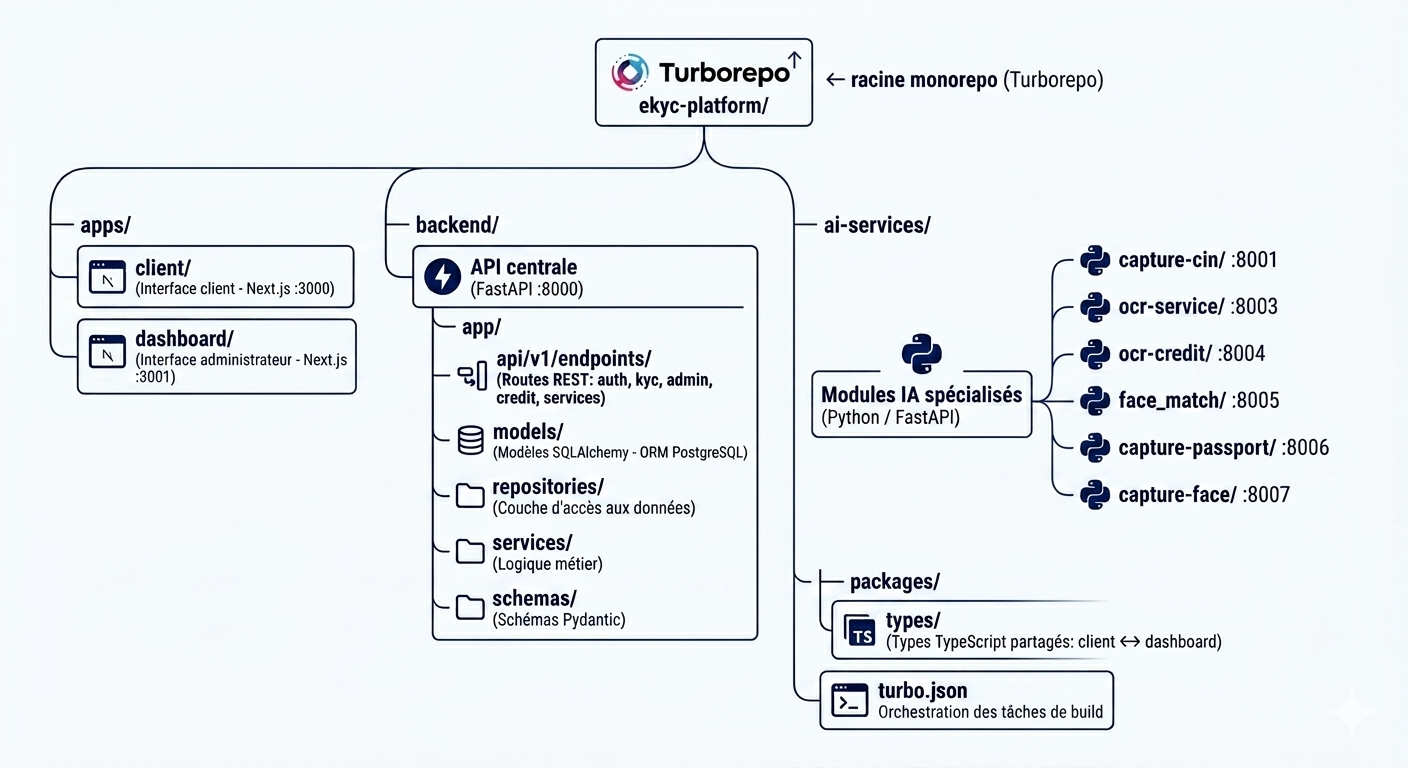
\includegraphics[width=0.95\textwidth]{images/image_ch5/archi_globale.png}
  \captionof{figure}{Architecture globale de la plateforme eKYC}
  \label{fig:ch6-archi-globale}
\end{center}
\vspace{0.6em}

La plateforme comprend deux applications frontend distinctes dont les métiers sont suffisamment différenciés pour justifier une séparation complète : l'une dédiée au parcours client, l'autre aux agents et superviseurs. Un backend central FastAPI orchestre les deux interfaces et prend en charge l'ensemble de la logique métier : gestion des dossiers KYC, authentification, filtrage AML et persistance. En complément, un système IA regroupe sept services spécialisés appelés directement par le frontend, indépendamment du backend. Les sections suivantes détaillent les points d'entrée de ce backend ainsi que les mécanismes de persistance sur lesquels il s'appuie.

\subsection{API REST --- Endpoints principaux}
\label{subsec:api-rest}

Le backend expose une API REST versionnée sous le préfixe \texttt{/api/v1}, organisée en six groupes de routes selon le domaine fonctionnel. Le Tableau~\ref{tab:api-routes} présente la vue d'ensemble de ces groupes.

\renewcommand{\arraystretch}{1.3}
\begin{longtable}{|p{2cm}|p{4cm}|p{6cm}|p{3cm}|}
  \rowcolor{bleu_principal}
  \textcolor{white}{\textbf{Groupe}} & \textcolor{white}{\textbf{Préfixe}} & \textcolor{white}{\textbf{Rôle}} & \textcolor{white}{\textbf{Acteur}} \\
  \hline
  \endfirsthead
  \rowcolor{bleu_principal}
  \textcolor{white}{\textbf{Groupe}} & \textcolor{white}{\textbf{Préfixe}} & \textcolor{white}{\textbf{Rôle}} & \textcolor{white}{\textbf{Acteur}} \\
  \hline
  \endhead
  \textbf{Auth}     & \texttt{/api/v1/auth}     & Authentification, inscription, gestion des tokens & Client + Admin \\
  \hline
  \textbf{KYC}      & \texttt{/api/v1/kyc}      & Soumission et suivi des demandes KYC              & Client \\
  \hline
  \textbf{Admin}    & \texttt{/api/v1/admin}    & Revue, validation, scoring, alertes AML           & Agent / Superviseur / Admin \\
  \hline
  \textbf{Crédit}   & \texttt{/api/v1/credit}   & Demandes de crédit bancaire                       & Client + Admin \\
  \hline
  \textbf{Services} & \texttt{/api/v1/services} & Demandes de carte bancaire et chéquier            & Client + Admin \\
  \hline
  \textbf{IA}       & \texttt{/api/v1/admin/ia} & Métriques IA en temps réel (monitoring)           & Superviseur \\
  \hline
  \caption{Vue d'ensemble des groupes de routes --- API REST}
  \label{tab:api-routes}
\end{longtable}

Ces six groupes de routes couvrent l'ensemble des interactions entre les interfaces et le backend. Les données produites par ces échanges — qu'il s'agisse de résultats OCR, de décisions d'agents ou de scores de risque — sont ensuite persistées dans les deux systèmes décrits ci-après.

\subsection{Persistance et stockage}
\label{subsec:persistance-stockage}

La plateforme repose sur deux systèmes de persistance complémentaires : \textbf{PostgreSQL} pour les données structurées et \textbf{MinIO} pour les fichiers binaires. Les deux sous-sections suivantes décrivent le rôle et le contenu de chacun.

\subsubsection{Base de données PostgreSQL}

PostgreSQL est la base de données relationnelle principale du système. Toutes les données métier y sont persistées : comptes utilisateurs, demandes KYC, résultats OCR, décisions administratives, journaux d'audit et listes de filtrage AML. Le Tableau~\ref{tab:bdd-tables} présente les tables principales du schéma.

\renewcommand{\arraystretch}{1.3}
\begin{longtable}{|p{5cm}|p{9.5cm}|}
  \rowcolor{bleu_principal}
  \textcolor{white}{\textbf{Table}} & \textcolor{white}{\textbf{Contenu}} \\
  \hline
  \endfirsthead
  \rowcolor{bleu_principal}
  \textcolor{white}{\textbf{Table}} & \textcolor{white}{\textbf{Contenu}} \\
  \hline
  \endhead
  \texttt{users}                       & Comptes utilisateurs (client, agent, superviseur, admin) \\ \hline
  \texttt{user\_information}           & Données d'identité KYC du client (nom, CIN, date de naissance...) \\ \hline
  \texttt{kyc\_demandes}               & Demandes KYC avec statut, type de compte, agent assigné, niveau de risque \\ \hline
  \texttt{kyc\_documents}              & Documents soumis (CIN recto/verso, passeport) avec URL MinIO \\ \hline
  \texttt{ocr\_results}                & Résultats bruts YOLO + PaddleOCR en JSONB (structured, raw\_detections, scores) \\ \hline
  \texttt{ocr\_corrections}            & Corrections manuelles des champs OCR (client ou agent) \\ \hline
  \texttt{selfies}                     & URLs MinIO des selfies capturés \\ \hline
  \texttt{face\_crops}                 & URLs MinIO des crops visage extraits par YOLO \\ \hline
  \texttt{validation\_scores}          & Score de risque global calculé par le backend \\ \hline
  \texttt{blacklist}                   & Liste noire AML (noms, CIN) \\ \hline
  \texttt{ppe\_list}                   & Liste des Personnes Politiquement Exposées \\ \hline
  \texttt{blacklist\_matches}          & Correspondances détectées entre un client et la blacklist \\ \hline
  \texttt{ppe\_matches}                & Correspondances PPE détectées \\ \hline
  \texttt{identity\_duplicate\_alerts} & Alertes de doublons biométriques ou d'identité entre dossiers \\ \hline
  \texttt{demand\_comments}            & Commentaires internes des agents sur les dossiers \\ \hline
  \texttt{audit\_logs}                 & Journal des actions sensibles (connexion, décision, modification) \\ \hline
  \texttt{audit\_views}                & Historique des consultations de dossiers par les agents \\ \hline
  \texttt{comptes\_bancaires}          & Comptes bancaires ouverts au nom des clients \\ \hline
  \texttt{demand\_credit}              & Demandes de crédit bancaire \\ \hline
  \texttt{demande\_carte}              & Demandes de carte bancaire \\ \hline
  \texttt{demande\_chequier}           & Demandes de chéquier \\ \hline
  \caption{Schéma des tables principales --- PostgreSQL}
  \label{tab:bdd-tables}
\end{longtable}

PostgreSQL centralise ainsi toutes les informations métier sous forme structurée. Les fichiers binaires associés à ces enregistrements sont quant à eux gérés par un système dédié, présenté ci-après.

\subsubsection{Stockage objet MinIO}

Si PostgreSQL gère les données structurées, les fichiers binaires — images de documents, selfies, crops de visage — sont pris en charge par MinIO. Dans le cadre de ce projet, MinIO est déployé en tant que serveur de stockage local dédié, simulant le comportement d'un serveur institutionnel tel que celui qu'une banque exploiterait en production pour archiver les documents sensibles de ses clients. Ce choix répond à une contrainte de sécurité fondamentale : aucune image ne doit transiter vers un service externe ou un stockage cloud tiers. Toutes les images restent confinées à l'infrastructure locale, garantissant la souveraineté des données conformément aux exigences du secteur bancaire.

MinIO expose une interface compatible S3 qui permet à chaque service IA d'y accéder directement via une URL interne. Chaque image capturée pendant le parcours KYC y est enregistrée dès sa production et référencée dans PostgreSQL par son adresse. Le Tableau~\ref{tab:minio-categories} présente les catégories d'images stockées.

\renewcommand{\arraystretch}{1.3}
\begin{longtable}{|p{4cm}|p{10cm}|}
  \rowcolor{bleu_principal}
  \textcolor{white}{\textbf{Catégorie}} & \textcolor{white}{\textbf{Contenu}} \\
  \hline
  \endfirsthead
  \rowcolor{bleu_principal}
  \textcolor{white}{\textbf{Catégorie}} & \textcolor{white}{\textbf{Contenu}} \\
  \hline
  \endhead
  Documents d'identité & Photos de la CIN (recto et verso) ou du passeport capturées par le client \\ \hline
  Selfies              & Photo du visage prise lors de l'étape de vérification biométrique \\ \hline
  Crops visage         & Zone du visage découpée automatiquement depuis le document d'identité \\ \hline
  Documents financiers & Attestations de salaire pour les demandes de crédit \\ \hline
  \caption{Catégories d'images stockées dans MinIO}
  \label{tab:minio-categories}
\end{longtable}

PostgreSQL et MinIO jouent ainsi des rôles complémentaires sans être directement connectés : PostgreSQL conserve les \textbf{informations} sur chaque dossier, MinIO conserve les \textbf{fichiers}. Le lien entre les deux se fait par les URLs — chaque image stockée dans MinIO est référencée dans PostgreSQL par son adresse. Lorsqu'un agent consulte un dossier, le backend récupère les métadonnées depuis PostgreSQL puis charge les images directement depuis MinIO. Cette complémentarité constitue le socle sur lequel repose l'intégration des services IA, décrite dans la section suivante.


%=============================================================
\section{Intégration des services IA}
\label{sec:integration-ia}
%=============================================================

L'infrastructure applicative étant posée, cette section décrit comment les services IA développés lors du premier incrément s'y intègrent pour former un système unifié. Elle présente d'abord la stratégie d'intégration par contrat d'interface, puis détaille les flux de communication effectifs entre chaque couche du système.

\subsection{De deux incréments à un système unifié}
\label{subsec:integration-increments}

Le développement de la plateforme eKYC a suivi deux incréments parallèles et complémentaires : un incrément dédié aux modules d'intelligence artificielle (capture, OCR, comparaison biométrique) et un incrément dédié au système applicatif (backend, interfaces client et administrateur, base de données). Menés de façon indépendante, ces deux incréments convergent à la soumission du dossier KYC pour former un \textbf{système eKYC unifié} : le pipeline IA produit les données d'identité et les scores biométriques, le système applicatif les reçoit, les persiste et les soumet à la décision d'un agent. La question centrale de l'intégration était de définir comment ces deux incréments allaient se rejoindre sans créer de dépendance forte entre eux. Les trois sous-sections suivantes décrivent respectivement le contrat d'interface retenu, le point de jonction effectif, et les bénéfices de cette approche.

\subsubsection{Le contrat d'interface comme point de jonction}

La décision fondamentale a été de définir un \textbf{contrat d'interface clair} entre les deux incréments avant même de commencer le développement. Ce contrat repose sur un principe simple : le système IA ne connaît pas le système applicatif, et le système applicatif ne connaît pas les modèles IA. Les deux communiquent uniquement par échange de données structurées (JSON) et d'adresses d'images (URLs MinIO), comme illustré par la Figure~\ref{fig:ch6-contrat-interface}.

\vspace{0.6em}
\begin{center}
  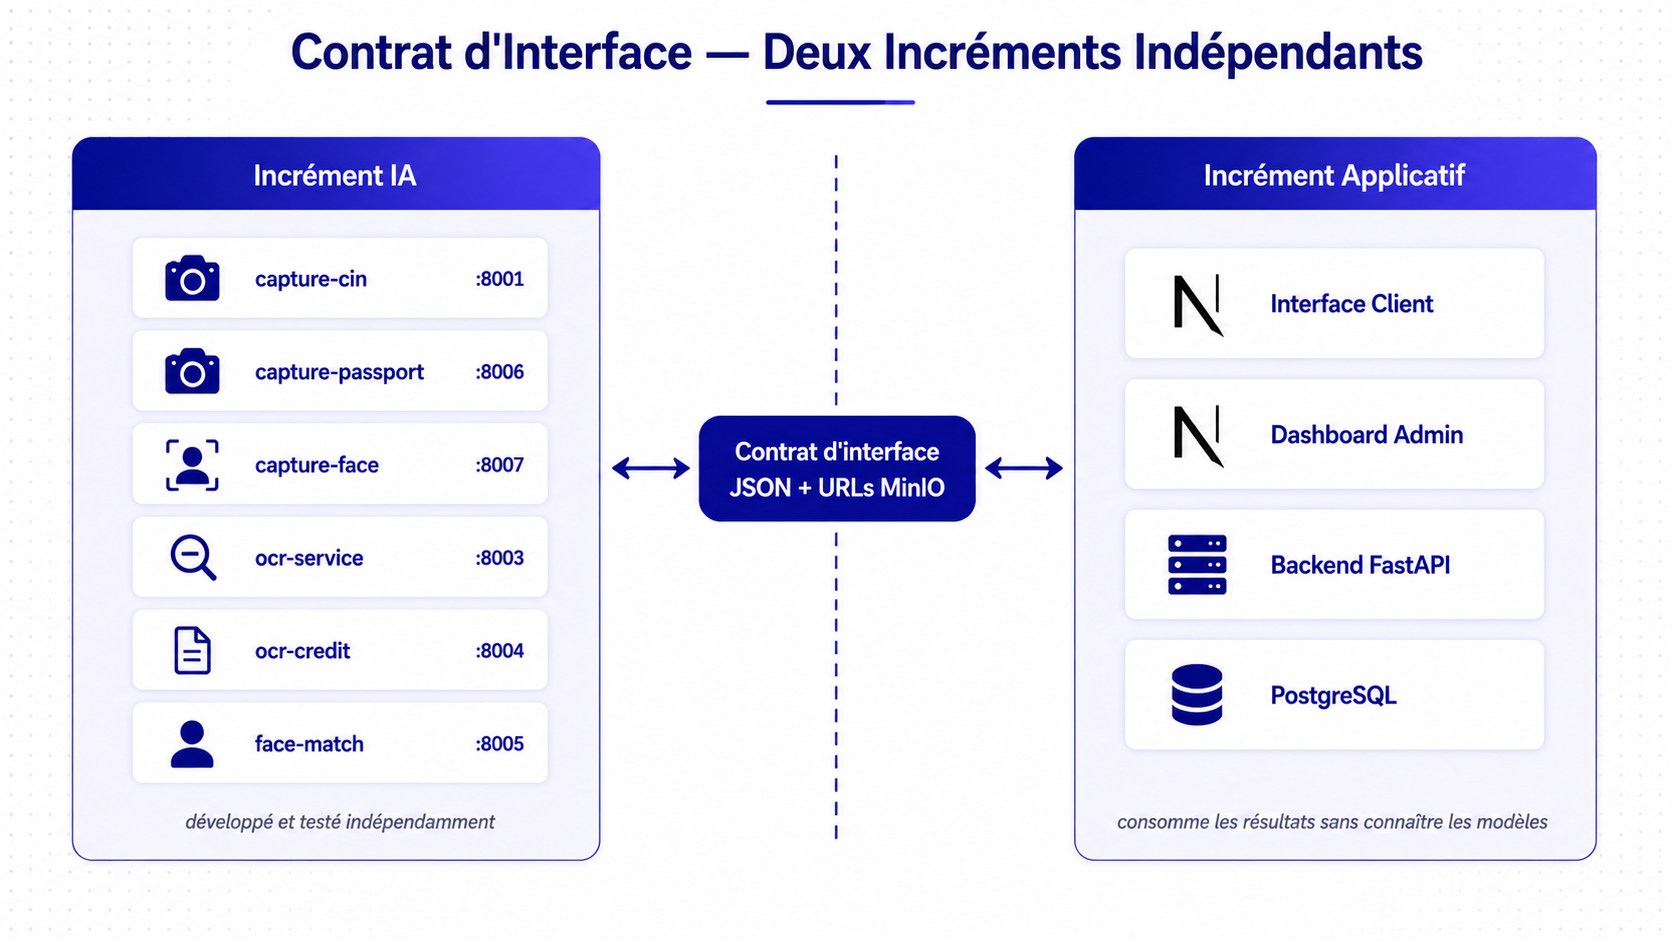
\includegraphics[width=0.95\textwidth]{images/image-ch6/Diagramme de contrat d'interface système.png}
  \captionof{figure}{Contrat d'interface entre le système IA et le système applicatif}
  \label{fig:ch6-contrat-interface}
\end{center}
\vspace{0.6em}

Concrètement, chaque module IA expose un endpoint précis avec un format de réponse fixe. Le système applicatif consomme ces réponses sans se préoccuper de ce qui se passe à l'intérieur du module. Ce découplage a permis aux deux incréments d'avancer indépendamment : le système applicatif pouvait être développé et testé avec des données simulées pendant que les modèles IA étaient encore en cours d'entraînement.

\subsubsection{Comment les deux incréments se rejoignent}

Fort de ce contrat d'interface, le point de jonction effectif entre les deux incréments est l'endpoint \texttt{POST /api/v1/kyc/submit-full} du backend. C'est à ce moment que les résultats produits par le système IA (données d'identité extraites, scores de confiance, URL du crop visage) sont transmis au système applicatif pour être persistés et soumis à la validation d'un agent, comme illustré par la Figure~\ref{fig:ch6-jonction-increments}.

\vspace{0.6em}
\begin{center}
  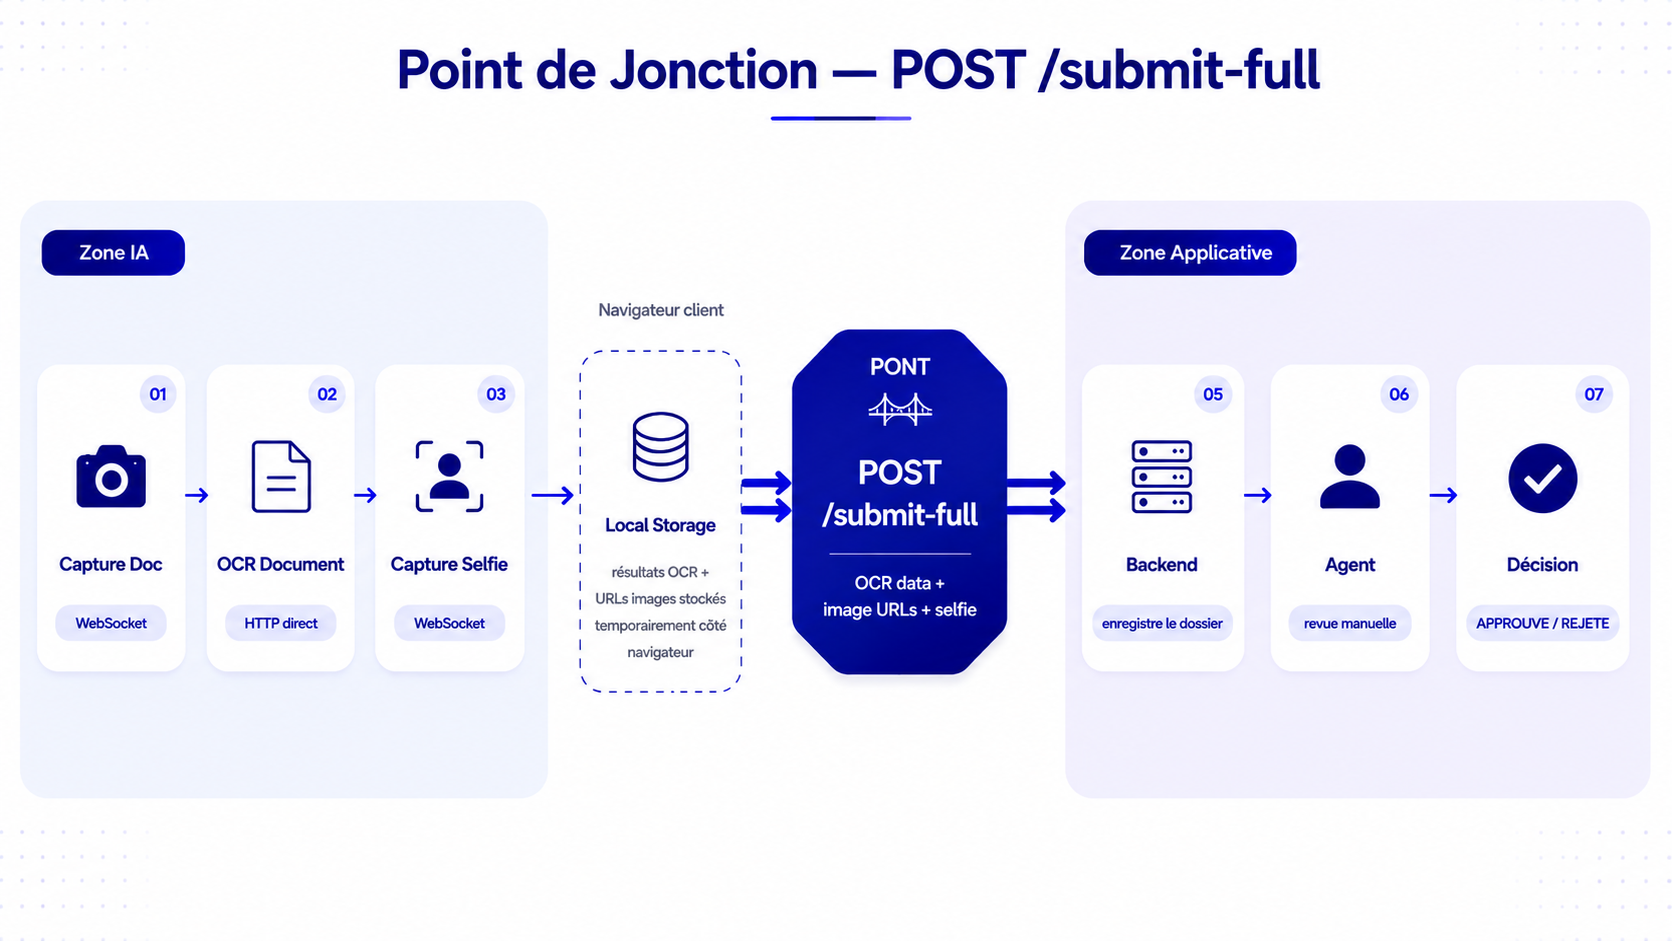
\includegraphics[width=0.95\textwidth]{images/image-ch6/ChatGPT Image 30 mai 2026, 03_02_18.png}
  \captionof{figure}{Point de jonction entre les deux incréments --- soumission finale du dossier KYC}
  \label{fig:ch6-jonction-increments}
\end{center}
\vspace{0.6em}

Jusqu'à ce point, l'interface client orchestre les appels aux modules IA, collecte leurs résultats étape par étape et les conserve localement. Ce n'est qu'à cet instant que le système applicatif prend le relais : il enregistre le dossier, assigne un agent et déclenche le processus de validation.

\subsubsection{Bénéfices de cette approche}

Ce mode d'intégration a apporté deux avantages concrets pendant le développement. D'abord, il a été possible de tester chaque incrément séparément : les modules IA pouvaient être évalués sur des jeux d'images indépendamment du backend, et le backend pouvait être développé avec des données OCR fictives avant que les vrais modèles soient prêts. Ensuite, cette séparation rend le système évolutif : remplacer un modèle OCR par une version plus performante ne nécessite aucune modification du backend, tant que le format de la réponse reste identique.

Cette stratégie d'intégration étant posée, la sous-section suivante détaille les flux de communication effectifs entre chaque couche du système au moment de l'exécution.

%-------------------------------------------------------------
\subsection{Communication entre les couches}
\label{subsec:communication-couches}

Au-delà du contrat d'interface qui définit les formats d'échange, le système IA est structuré en un ensemble de modules indépendants, chacun accessible via une adresse réseau locale dédiée. Cette organisation permet de faire évoluer, remplacer ou redémarrer un module sans affecter les autres composants du système. La Figure~\ref{fig:ch6-communication-ia} illustre les flux de communication entre chaque couche, présentés dans les paragraphes qui suivent.

\vspace{0.6em}
\begin{center}
  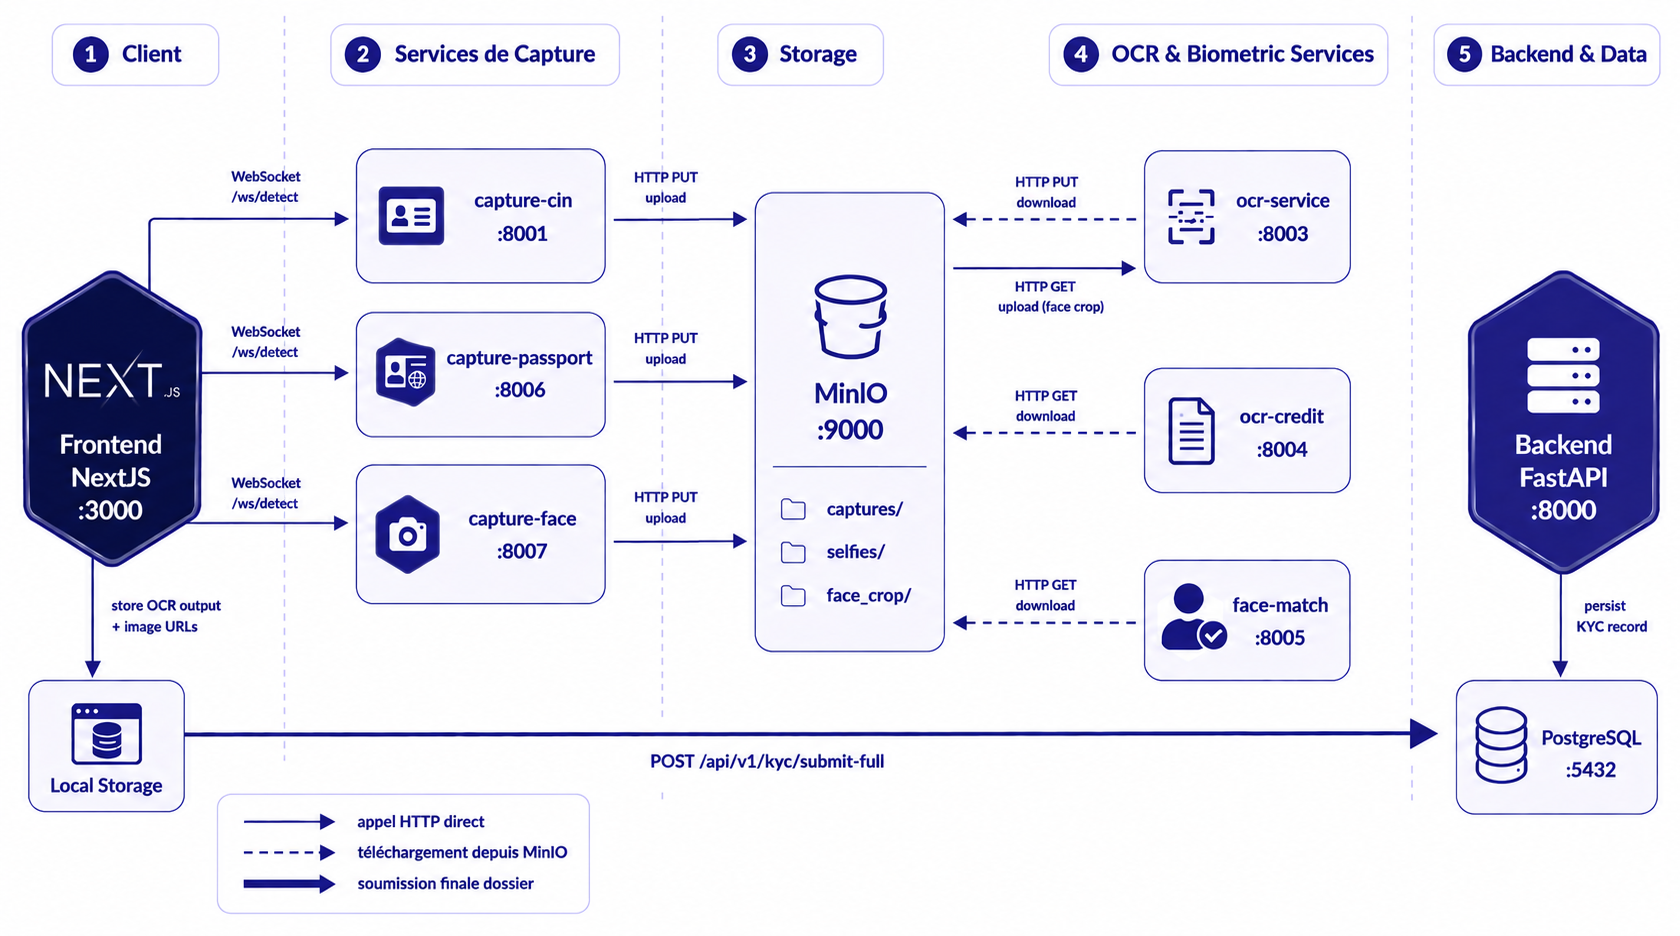
\includegraphics[width=0.95\textwidth]{images/image_ch5/communicationIa.png}
  \captionof{figure}{Schéma de communication entre les couches de la plateforme eKYC}
  \label{fig:ch6-communication-ia}
\end{center}
\vspace{0.6em}

\paragraph{L'interface client}
est le point de départ de toutes les interactions. Elle contacte directement les modules de capture pour guider le client devant sa caméra, puis les modules OCR pour extraire les informations des documents photographiés, sans jamais passer par le backend pour ces opérations. Ce choix réduit la latence et évite de surcharger le serveur central avec des flux vidéo ou des images volumineuses.

\paragraph{Les modules de capture}
(CIN, passeport, selfie) reçoivent les images de la caméra en temps réel, détectent la présence et la qualité du document dans le cadre, et déposent l'image directement dans MinIO une fois la capture validée par le client. Ils retournent à l'interface l'adresse URL de l'image stockée, sans jamais transmettre l'image elle-même au backend.

\paragraph{Les modules OCR}
reçoivent ces adresses d'images depuis l'interface, téléchargent les images depuis MinIO, analysent le document pour en extraire les champs textuels, et retournent les données structurées à l'interface. Le résultat est conservé temporairement côté client jusqu'à la soumission du dossier.

\paragraph{Le backend}
n'intervient qu'à deux moments précis : lors de la soumission du dossier, où il reçoit en une seule requête l'ensemble des données collectées par l'interface ; et lors de la validation par un agent, où il sollicite le module de comparaison biométrique.

\paragraph{Le module de comparaison biométrique}
est le seul service IA appelé exclusivement par le backend : il compare le visage extrait du document avec le selfie pour détecter toute tentative d'usurpation d'identité entre plusieurs dossiers.

MinIO joue un rôle transversal à l'ensemble de ces échanges, comme détaillé ci-après.

\subsubsection{Rôle de MinIO comme intermédiaire universel}

Transversalement à toutes ces couches, MinIO constitue le seul point de passage des images entre tous les acteurs du système. Aucune image n'est transmise directement d'un service à un autre sous forme de fichier — chaque composant dépose ou récupère les images via MinIO en utilisant une adresse URL. Cette approche simplifie les échanges, évite de transférer des fichiers volumineux dans les requêtes réseau, et garantit que chaque image est archivée de façon centralisée dès sa création.

%=============================================================
\section{Interface client}
\label{sec:interface-client}
%=============================================================

% [Contenu à rédiger ultérieurement]


%=============================================================
\section{Interface administrateur}
\label{sec:interface-admin}
%=============================================================

% [Contenu à rédiger ultérieurement]



\section*{Conclusion du chapitre}

Ce chapitre a présenté la réalisation complète de la plateforme eKYC, de l'infrastructure applicative jusqu'à l'intégration des services IA. L'ensemble des composants développés dans les deux incréments --- le pipeline d'intelligence artificielle d'une part, et le système applicatif d'autre part --- se rejoignent à la soumission finale du dossier pour former un \textbf{système eKYC unifié et opérationnel} : le client est guidé par le pipeline IA à chaque étape de capture, ses données sont extraites et vérifiées automatiquement, puis transmises au backend qui orchestre la validation par un agent selon les exigences de la Banque Centrale de Tunisie. Le résultat est une plateforme cohérente, où les deux incréments ne font plus qu'un seul système au service du parcours d'ouverture de compte.


% ============================================================
% CONCLUSION GÉNÉRALE
% ============================================================

\chapter*{Conclusion Générale}
\addcontentsline{toc}{chapter}{Conclusion Générale}

\section*{Bilan des réalisations}

\section*{Limites du projet}

\section*{Perspectives}

\bibliographystyle{plain}
\bibliography{references}

\end{document}
